% ============================================================================
% 08_previsao_ocorrencia.tex
% Capítulo: Reformulação do problema para PREVISÃO DE OCORRÊNCIA de fogo
% observado. Inserir via % ============================================================================
% 08_previsao_ocorrencia.tex
% Capítulo: Reformulação do problema para PREVISÃO DE OCORRÊNCIA de fogo
% observado. Inserir via % ============================================================================
% 08_previsao_ocorrencia.tex
% Capítulo: Reformulação do problema para PREVISÃO DE OCORRÊNCIA de fogo
% observado. Inserir via % ============================================================================
% 08_previsao_ocorrencia.tex
% Capítulo: Reformulação do problema para PREVISÃO DE OCORRÊNCIA de fogo
% observado. Inserir via \input{08_previsao_ocorrencia} no tcc.tex, APÓS o
% Capítulo 5 (Resultados, que termina com \input{07_estudo_caso_pium_to}) e
% ANTES do \chapter{Conclusão}. Torna-se o Capítulo 6; a Conclusão passa a 7.
% Números conferem com modelos/relatorios/previsao_ocorrencia_*.json,
% benchmark_p3_fwi.json, driver_*.json, comparacao_familias.json,
% validacao_rotulo_mapbiomas.json.
% ============================================================================

\chapter{Previsão de ocorrência de fogo: reformulação do problema}
\label{cap:ocorrencia}

O Capítulo~\ref{cap:metodologia} e o Apêndice~\ref{cap:resultados} descrevem uma abordagem
exploratória inicial: um classificador de \emph{nível de risco em tempo real}
(\emph{nowcast}) cujo alvo é o índice Risco de Fogo do INPE discretizado em três faixas. Este capítulo reformula o problema para a
\textbf{previsão de ocorrência de fogo observado}, com horizonte temporal explícito,
classe negativa real e validação sem vazamento --- alinhando o trabalho ao estado da arte
atual, que prevê o \emph{fenômeno observado} (focos ou área queimada), e não a saída de
outro modelo~\cite{huot2022nextday,karasante2025firecastnet,deandrade2024lstmgru}. O
\emph{pipeline} original é mantido como linha de base; o reformulado constitui a principal
contribuição metodológica desta etapa.

\section{Motivação: do índice ao fenômeno observado}
\label{sec:oco_motivacao}

A inspeção dos dados revelou três fragilidades de fundo na formulação original.
Primeiro, o alvo (\texttt{RiscoFogo}) é a \textbf{saída de um índice operacional} do INPE,
ele próprio derivado de dias sem chuva, precipitação e umidade --- variáveis que também
figuram entre as \emph{features}, gerando circularidade. Segundo, a base é
\emph{presence-only}: as \num{924306} linhas são focos reais, sem exemplos de
\emph{não-fogo}; o modelo nunca aprende a distinguir fogo de ausência de fogo, e a consulta
a pontos arbitrários no aplicativo equivale a extrapolar para fora do suporte de treino.
Terceiro, trata-se de um \emph{nowcast} (diagnóstico do presente), não de previsão com
horizonte.

Há evidência empírica direta nos próprios CSVs do INPE: em um único arquivo anual
(\num{82678} focos), \num{8288} detecções (\(\approx\)\SI{10}{\percent}) ocorreram onde o
índice marcava risco mínimo (\texttt{RiscoFogo}~\(\in\{0{,}0;\,0{,}1\}\)) --- fogo real em
locais classificados como ``Baixo''. Um modelo que imita o índice herda esse ponto cego,
exatamente o que o estudo de caso Pium--TO (Seção~\ref{sec:res_estudo_caso_pium}) demonstrou.

\section{Reformulação metodológica}
\label{sec:oco_metodo}

\paragraph{Unidade e alvo.} Adota-se uma grade de células de \SI{0,25}{\degree}
(\(\approx\)\SI{27}{km}, granularidade MERRA-2/SeasFire~\cite{karasante2025firecastnet}) por
mês. O universo é o conjunto de \num{4168} células \emph{fire-prone} (com \(\geq 1\) foco em
2014--2023). Para cada par (célula, mês~\(t\)), o alvo é binário: \emph{houve foco no mês
\(t+1\)?} A presença vem dos focos observados; a \textbf{ausência} (classe negativa antes
inexistente) são os pares célula--mês sem foco. O conjunto final tem \num{450144}
células--mês (2015--2023), com prevalência de \SI{24,7}{\percent}.

\paragraph{Amostragem da classe negativa.} Construir a classe negativa a partir dos pares
célula--mês sem foco é uma decisão de projeto, não uma escolha neutra: na modelagem de
distribuição (\emph{species distribution models}), a definição e o volume das
\emph{pseudo-ausências}/\emph{background} afetam o desempenho aparente e podem inflar métricas
como a AUC quando o \emph{background} é ``fácil''~\cite{barbetmassin2012pseudo,phillips2009sample,lobo2008auc}.
Aqui a prevalência é fixada pelo próprio domínio (\SI{24,7}{\percent} de positivos entre as
células \emph{fire-prone}), evitando o desbalanceamento extremo em que a AUC se torna
enganosa; para métodos baseados em árvores, poucos negativos com ponderação de classes bastam~\cite{barbetmassin2012pseudo},
e adota-se \texttt{class\_weight=balanced}. Uma checagem com negativos restritos por
similaridade geográfica (evitando pares triviais)~\cite{xu2023nonfire} fica registrada como
refinamento --- direção que torna o problema mais realista, não mais fácil.

\paragraph{Causalidade e validação.} Para eliminar o vazamento temporal documentado na
Seção~\ref{sec:res_temporal}, todas as \emph{features} usam apenas informação \(\leq t\)
(histórico de fogo defasado, somas móveis com deslocamento, sazonalidade, localização). A
validação é \textbf{espaço-temporal em bloco}~\cite{roberts2017cv}: \emph{rolling-origin} por
ano (treino \(<Y\), teste \(=Y\), para \(Y\in\{2021,2022,2023\}\)) e \emph{leave-region-out}
(5 blocos de longitude). A métrica principal é a \textbf{PR-AUC} (\emph{Average Precision}),
robusta ao desbalanceamento.

\section{Desempenho preditivo e linhas de base}
\label{sec:oco_desempenho}

O modelo (\emph{Hist\-Gradient\-Boosting}) supera as linhas de base de persistência e
climatologia (Tabela~\ref{tab:oco_validacao}). Na validação \emph{espacial}, a climatologia
colapsa ao prever regiões nunca vistas (PR-AUC \numrange{0,17}{0,34}), enquanto o modelo
mantém \num{0,759} --- evidência de dinâmica transferível, e não de memorização de taxa-base
local (contraste direto com a dependência espacial observada no \emph{pipeline} original).

\begin{table}[h]
\centering
\caption{Previsão de ocorrência (fogo em \(t+1\)): validação em bloco vs.\ linhas de base.}
\label{tab:oco_validacao}
\small
\begin{tabular}{lcccc}
\toprule
\textbf{Validação} & \textbf{Modelo PR-AUC} & \textbf{ROC-AUC} & \textbf{Persistência} & \textbf{Climatologia} \\
\midrule
Temporal (\emph{rolling-origin} 2021--23) & \textbf{0,777} & 0,904 & 0,449 & 0,715 \\
Espacial (\emph{leave-region-out}) & \textbf{0,759} & 0,895 & --- & 0,17--0,34 \\
\bottomrule
\end{tabular}
\end{table}

\paragraph{Escolha da métrica.} A PR-AUC é adotada como métrica principal por ser sensível à
classe positiva rara: sob desbalanceamento, a ROC-AUC pode permanecer alta e mascarar a queda
de precisão que a curva \emph{precision-recall} revela~\cite{saito2015precision,davis2006relationship}.
Reportam-se também ROC-AUC e Brier. Registra-se, por completude, que a superioridade
incondicional da PR-AUC foi formalmente questionada~\cite{mcdermott2024closer}: a escolha aqui
segue o \emph{objetivo operacional} (priorizar a detecção do fogo, evento raro e de alto custo
de omissão), não uma preferência a priori.

\paragraph{Área de aplicabilidade.} A validação \emph{leave-region-out} mede a generalização a
regiões não vistas, mas predições fora do envelope de \emph{features} do treino permanecem
menos confiáveis. A delimitação formal da \textbf{área de aplicabilidade}~\cite{meyer2021aoa}
--- restringindo o mapa às células suficientemente similares ao conjunto de treino --- é o
complemento recomendado para o uso operacional do produto.

\section{Robustez entre famílias de modelo}
\label{sec:oco_familias}

Para verificar que os achados não dependem do algoritmo, quatro famílias foram comparadas no
mesmo conjunto de \emph{features}, com intervalos de confiança de \SI{95}{\percent} obtidos
por \emph{cluster bootstrap} por célula (respeitando a autocorrelação espacial),
Tabela~\ref{tab:oco_familias}. Os \emph{ensembles} de árvore são estatisticamente
equivalentes (intervalos sobrepostos), enquanto a regressão logística é significativamente
inferior --- o problema exige não-linearidades. O \emph{Random Forest} apresenta a melhor
calibração (menor Brier).

\begin{table}[h]
\centering
\caption{Comparação de famílias (conjunto base + desmatamento), IC \SI{95}{\percent} por \emph{cluster bootstrap} por célula.}
\label{tab:oco_familias}
\small
\begin{tabular}{lcccc}
\toprule
\textbf{Família} & \textbf{PR-AUC [IC 95\%]} & \textbf{ROC-AUC} & \textbf{Brier} & \textbf{Nova ignição [IC 95\%]} \\
\midrule
\emph{HistGradientBoosting} & \textbf{0,776 [0,769--0,783]} & 0,904 & 0,123 & \textbf{0,232 [0,209--0,258]} \\
\emph{Random Forest} & 0,769 [0,762--0,776] & 0,901 & \textbf{0,113} & 0,204 [0,185--0,232] \\
\emph{Extra Trees} & 0,761 [0,754--0,768] & 0,897 & 0,129 & 0,191 [0,174--0,217] \\
Regressão Logística & 0,699 [0,690--0,707] & 0,873 & 0,143 & 0,117 [0,108--0,131] \\
\bottomrule
\end{tabular}
\end{table}

\section{Benchmark contra índices físicos de perigo de fogo}
\label{sec:oco_benchmark}

A defensabilidade da tese exige que o modelo \emph{supere} o índice físico operacional na
previsão de fogo observado. Implementou-se o \textbf{Fire Weather Index (FWI)} canadense
completo~\cite{vanwagner1985fwi} --- base do sistema GEFF/EFFIS do
Copernicus~\cite{digiuseppe2024geff} ---, validado contra os valores de referência publicados
(FFMC~\num{87,69}; DMC~\num{8,55}; DC~\num{19,01}; ISI~\num{10,85}; BUI~\num{8,49};
FWI~\num{10,10}). O FWI foi computado dia a dia a partir de clima diário (NASA POWER) para
uma amostra de \num{100} células. A Tabela~\ref{tab:oco_benchmark} mostra o resultado:
\textbf{o modelo de ML supera o FWI e o índice do INPE} na previsão de fogo observado. O FWI
separa fisicamente bem (média \num{6,0} em meses com fogo vs.\ \num{1,5} sem), validando a
implementação.

\begin{table}[h]
\centering
\caption{Benchmark de previsão de fogo observado (\(t+1\)): ML vs.\ índices físicos.}
\label{tab:oco_benchmark}
\small
\begin{tabular}{lcc}
\toprule
\textbf{Preditor} & \textbf{PR-AUC} & \textbf{ROC-AUC} \\
\midrule
Modelo ML (dataset completo) & \textbf{0,777} & 0,904 \\
Índice INPE Risco de Fogo (como \emph{forecast}) & 0,294 & 0,553 \\
\midrule
\multicolumn{3}{l}{\emph{Amostra de 100 células (2023), mesmas linhas:}} \\
\quad Modelo ML & \textbf{0,858} & --- \\
\quad FWI canadense (clima diário NASA POWER) & 0,608 & 0,781 \\
\quad Índice INPE Risco de Fogo & 0,398 & --- \\
\bottomrule
\end{tabular}
\end{table}

\section{Quantificação de incerteza por \emph{conformal prediction}}
\label{sec:oco_conformal}

Substituiu-se a heurística de incerteza por \emph{conjuntos de predição com cobertura
estatística garantida}, via \emph{split-conformal} classe-condicional
(LAC)~\cite{sadinle2019lac,mortier2024conformal}. Com cobertura-alvo de \SI{90}{\percent},
obteve-se cobertura empírica de \SI{88,8}{\percent}; \SI{82,9}{\percent} das predições são
\emph{singletons} confiantes e \SI{17,1}{\percent} são sinalizadas como ambíguas. O erro de
calibração esperado (ECE) foi de \num{0,099} e o \emph{Brier} de \num{0,123}.

\paragraph{Pressuposto e ressalva.} A garantia de cobertura do \emph{split-conformal} assume
\emph{permutabilidade} (\emph{exchangeability}) entre calibração e teste~\cite{angelopoulos2021gentle}.
A grade espaço-temporal viola parcialmente esse pressuposto (autocorrelação entre células e
meses vizinhos), o que é coerente com a leve subcobertura observada (\SI{88,8}{\percent} ante o
alvo de \SI{90}{\percent}). Sob desvio de distribuição, a cobertura nominal pode ser restaurada
por \emph{conformal} ponderado/adaptado~\cite{tibshirani2019conformal}; uma calibração com
particionamento espacial é o encaminhamento indicado para o uso operacional.

\section{Drivers antrópicos: o papel do desmatamento}
\label{sec:oco_drivers}

A análise estratificada revela a estrutura do problema (Tabela~\ref{tab:oco_estrato}): o
modelo é excelente onde o fogo \emph{recorre} (PR-AUC \num{0,805}) e fraco onde o fogo é
\emph{novo} --- a \textbf{nova ignição} (PR-AUC \num{0,230}), justamente o caso crítico para
alerta precoce, onde a persistência é inútil por construção.

\begin{table}[h]
\centering
\caption{Desempenho estratificado por recorrência (teste 2023) e ganho do desmatamento.}
\label{tab:oco_estrato}
\small
\begin{tabular}{lccc}
\toprule
\textbf{Estrato (média 2021--23)} & \textbf{base PR-AUC} & \textbf{+ desmatamento} & \textbf{\(\Delta\)} \\
\midrule
Recorrente (foco nos últimos 12 m) & 0,791 & 0,794 & +0,003 \\
\textbf{Nova ignição} (sem foco recente) & \textbf{0,206} & \textbf{0,231} & \textbf{+0,025} \\
Geral & 0,777 & 0,781 & +0,003 \\
\bottomrule
\end{tabular}
\end{table}

Testaram-se três famílias de covariáveis. O clima real (reanálise NASA POWER) e o FWI
\textbf{não agregam} sobre o histórico de fogo na escala mensal (\(\Delta\)~PR-AUC
\(\approx\)\num{+0,001}), pois o histórico já é um \emph{proxy} a jusante da propensão
climática. A distância a cidades (acessibilidade estática) também é redundante
(\(\approx\)\num{+0,001}). Apenas o \textbf{desmatamento recente} (PRODES, do
TerraBrasilis~\cite{terrabrasilisprodes}) agrega valor não trivial --- e \emph{exatamente}
no estrato de nova ignição (\(+0{,}025\) PR-AUC), confirmando o mecanismo causal: o
desmatamento precede a primeira queimada de uma célula, coerente com o fogo amazônico ser
majoritariamente antrópico~\cite{aragao2018amazon}. O achado é \textbf{robusto a duas fontes
independentes}: o DETER (alertas mensais; classe \emph{cicatriz de queimada} excluída para
evitar vazamento) produz ganho equivalente (\(+0{,}026\)). A resolução mensal não amplificou
o ganho, e dimensões adicionais (idade, estoque acumulado, fronteira de vizinhança) não
agregam além do volume de desmatamento recente local: o desempenho na nova ignição satura em
\(\approx\)\num{0,23} PR-AUC --- um teto que sugere componente irredutível (decisão humana) ou
necessidade de dados de outra natureza.

\section{Validação do rótulo contra área queimada (MapBiomas Fogo)}
\label{sec:oco_mapbiomas}

O rótulo (focos INPE) foi confrontado com um produto independente e de modalidade diferente
--- a área queimada do MapBiomas Fogo~\cite{mapbiomasfogo} (cicatriz Landsat \SI{30}{m}), em
dois níveis.

\paragraph{Nível estado/ano.} Correlacionando a contagem de focos com a área queimada por
(estado da Amazônia Legal, ano), 2014--2023, a concordância \textbf{interanual dentro de cada
estado} é forte (Spearman médio \num{0,814}; 9/9 estados positivos, \numrange{0,69}{0,94}):
quando a área queimada de um estado sobe num ano, os focos sobem junto. A correlação
\emph{entre} estados é fraca (\(\rho=\)\num{0,275}), pois a contagem de focos não é
\emph{proxy} linear da magnitude em hectares --- o que não afeta o rótulo aqui, por ser de
\textbf{ocorrência binária} e não de magnitude.

\paragraph{Nível célula \(\times\) ano.} Para a validação no nível da célula, leram-se os
rasters anuais do MapBiomas (COGs públicos, 2015--2020) via leitura remota por janelas,
binarizando a presença de cicatriz por célula \SI{0,25}{\degree}. Confrontando presença de
foco vs.\ presença de cicatriz em \num{23982} célula-anos: concordância de \SI{78}{\percent},
Cohen's \(\kappa=\num{0,33}\) e, tratando a cicatriz como referência, os focos têm
\textbf{revocação \num{0,90}} e precisão \num{0,83} (F\(_1=\num{0,86}\)). Ou seja, os focos
capturam \(\approx\)\SI{90}{\percent} dos célula-anos efetivamente queimados; as discordâncias
correspondem a fogos sem cicatriz detectável (pequenos/encobertos por nuvem) e a cicatrizes
sem foco coincidente (omissão da detecção ativa). O \(\kappa\) moderado reflete a alta
prevalência do universo \emph{fire-prone}, que comprime a concordância esperada por acaso. A
validação corrobora o rótulo de ocorrência tanto na dinâmica temporal quanto no nível espacial.

\section{Avaliação operacional e horizonte de previsão}
\label{sec:oco_operacional}

\paragraph{Priorização de alertas.} Para traduzir o desempenho em valor de decisão,
o sistema é avaliado como ferramenta de \emph{priorização}: dado um orçamento de
vigilância (alertar as \emph{top-K\%} células de maior risco previsto), quantos focos
do mês seguinte são capturados (\emph{recall@K})? A Tabela~\ref{tab:oco_operacional} e a
Figura~\ref{fig:oco_recallk} comparam o modelo de ML com o índice operacional do INPE
sob o mesmo orçamento. Alertando apenas \SI{10}{\percent} das células, o modelo captura
\SI{36,0}{\percent} dos focos do mês seguinte (com precisão de \SI{88}{\percent}), contra
\SI{15,8}{\percent} do índice INPE --- um ganho de \(\approx 2{,}3\times\). No estrato de
\textbf{nova ignição}, o contraste é decisivo: o modelo captura \SI{49,2}{\percent} dos
novos focos no mesmo orçamento (\emph{lift} de \(4{,}9\times\) sobre o acaso), ao passo que
o índice INPE tem \emph{lift} \(\approx 1\) --- ou seja, \emph{não supera o acaso} para a
nova ignição, justamente o regime em que o desmatamento recente é o sinal preditivo
(Seção~\ref{sec:oco_drivers}).

\begin{table}[h]
\centering
\caption{Priorização de alertas: \emph{recall@K} (focos do mês seguinte capturados) por orçamento, modelo ML vs.\ índice INPE.}
\label{tab:oco_operacional}
\small
\begin{tabular}{lcccc}
\toprule
& \multicolumn{2}{c}{\textbf{Global}} & \multicolumn{2}{c}{\textbf{Nova ignição}} \\
\cmidrule(lr){2-3}\cmidrule(lr){4-5}
\textbf{Orçamento (top-K\%)} & \textbf{ML} & \textbf{INPE} & \textbf{ML} & \textbf{INPE} \\
\midrule
\SI{5}{\percent}  & 0,195 & 0,071 & 0,312 & 0,041 \\
\SI{10}{\percent} & \textbf{0,360} & 0,158 & \textbf{0,492} & 0,096 \\
\SI{20}{\percent} & 0,611 & 0,282 & 0,721 & 0,206 \\
\SI{30}{\percent} & 0,775 & 0,372 & 0,845 & 0,305 \\
\bottomrule
\end{tabular}
\end{table}

\begin{figure}[h]
\centering
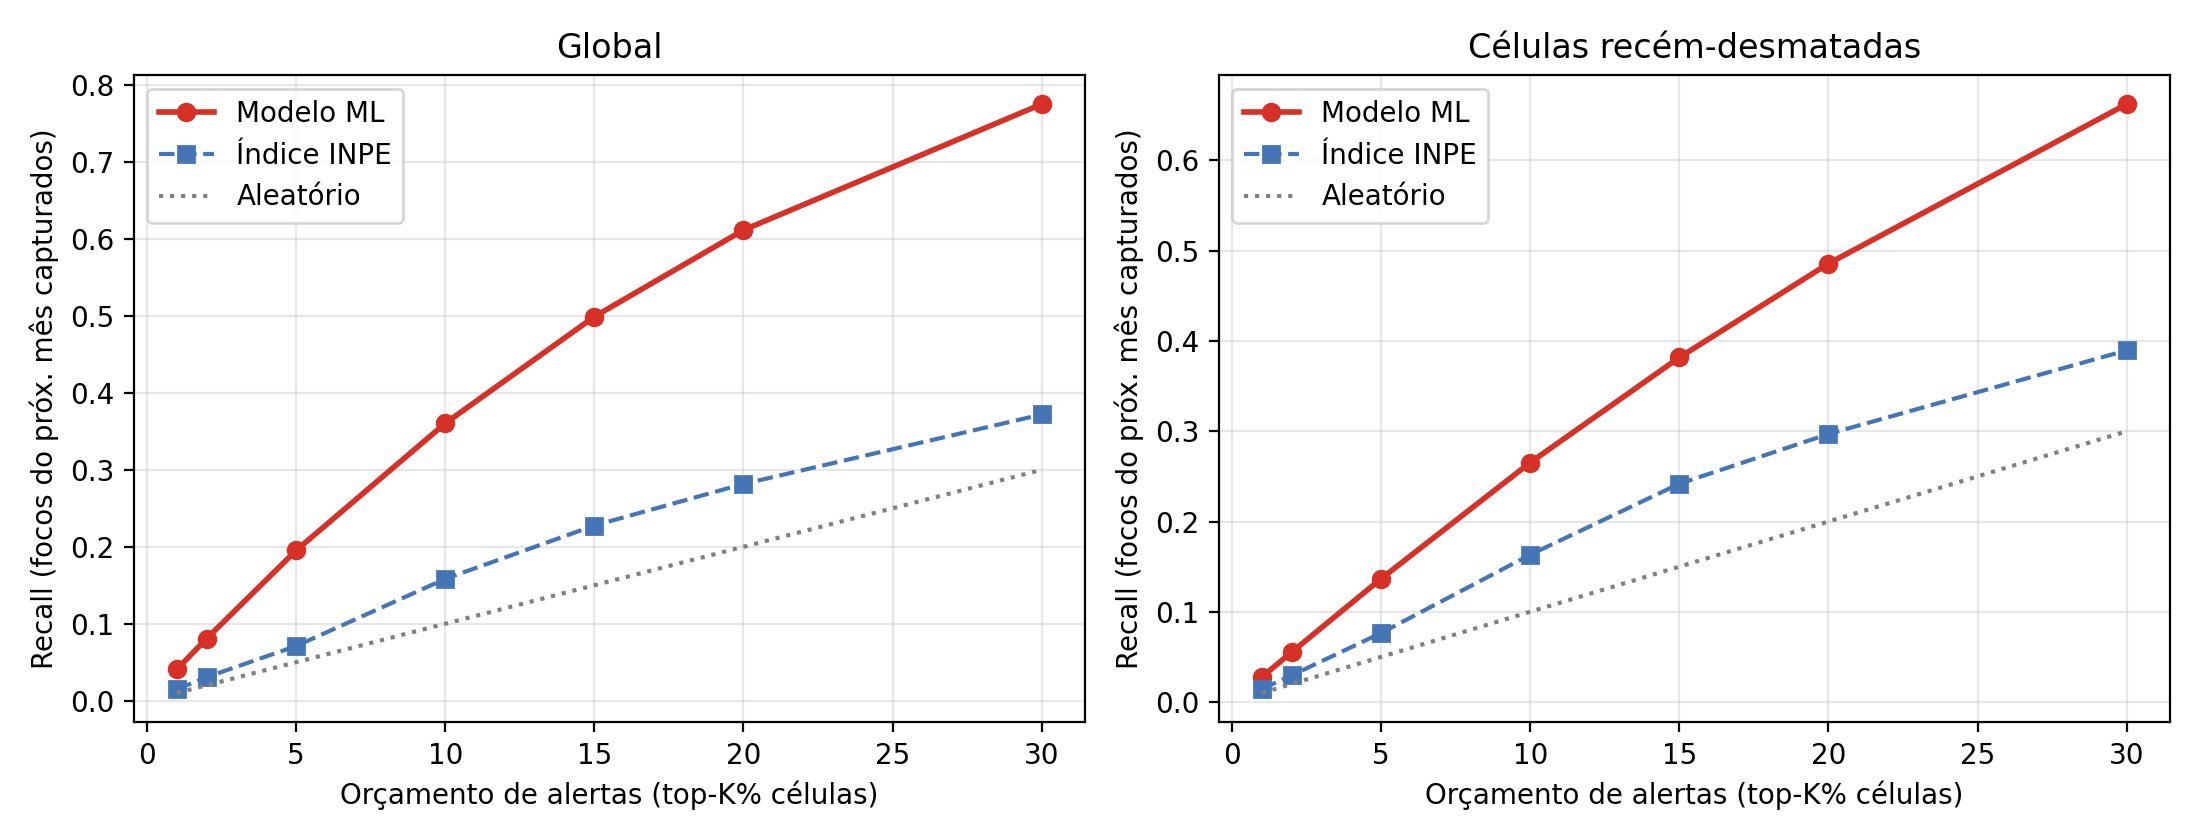
\includegraphics[width=\textwidth]{modelos/relatorios/avaliacao_operacional_recall_k.png}
\caption{\emph{Recall@K} em função do orçamento de alertas (modelo ML vs.\ índice INPE vs.\ aleatório), global (esq.) e em células recém-desmatadas (dir.).}
\label{fig:oco_recallk}
\end{figure}

\paragraph{Horizonte de previsão.} Estendendo o alvo para \(t+2\) e \(t+3\) meses, o
\emph{skill} permanece \textbf{estável} (PR-AUC \numlist{0,779;0,779;0,781} para \(t+1\),
\(t+2\), \(t+3\); Figura~\ref{fig:oco_horizonte}), sem o decaimento típico. Isso confirma
que a ocorrência mensal de fogo é governada por componentes \emph{lentos} (sazonalidade,
histórico de fogo, desmatamento), e não por dinâmica meteorológica de curto prazo ---
um resultado operacionalmente favorável, pois fornece \textbf{até um trimestre de
antecedência} sem perda de desempenho. A contrapartida honesta é que o modelo captura o
regime sazonal/persistente, não a dinâmica sub-mensal; previsões em escala mais fina
exigiriam outra formulação.

\begin{figure}[h]
\centering
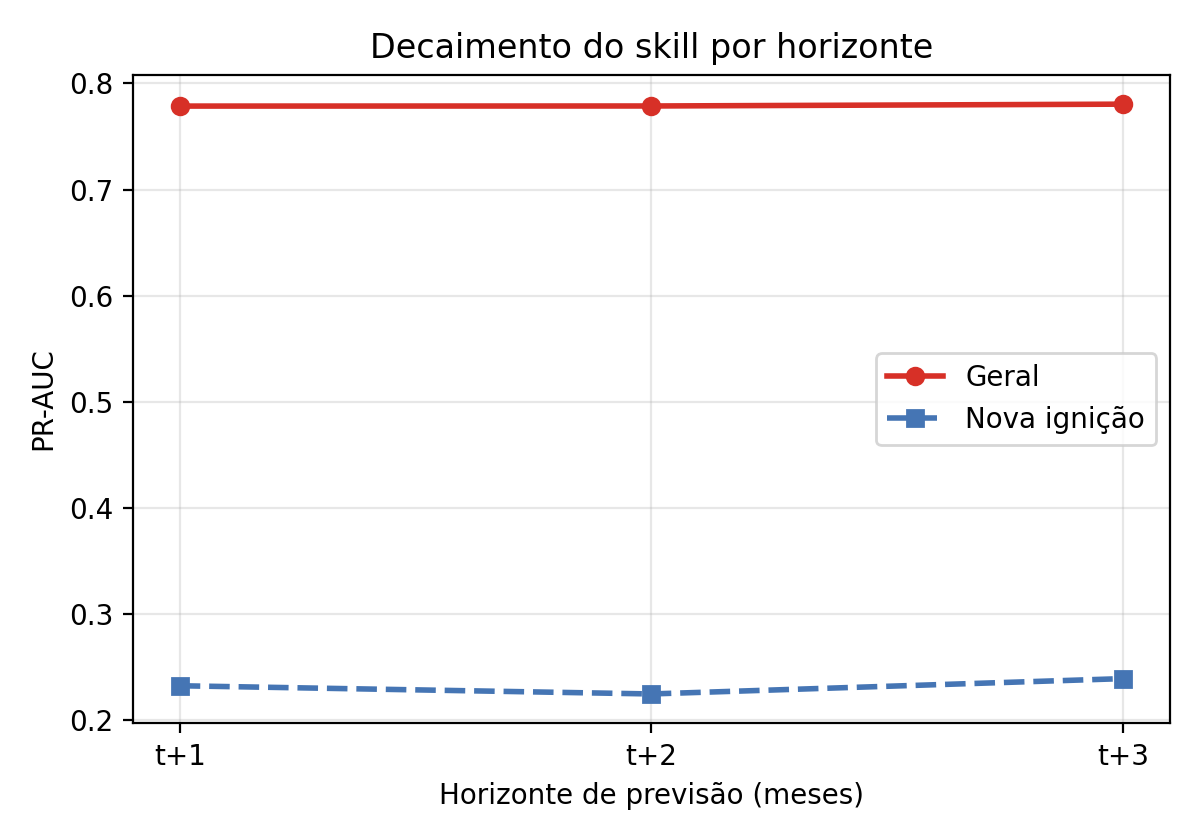
\includegraphics[width=0.6\textwidth]{modelos/relatorios/avaliacao_horizonte.png}
\caption{Decaimento do \emph{skill} (PR-AUC) por horizonte de previsão (\(t+1\) a \(t+3\) meses): estável, geral e na nova ignição.}
\label{fig:oco_horizonte}
\end{figure}

\section{Integração ao produto}
\label{sec:oco_produto}

O modelo final (base + desmatamento) foi serializado, calibrado por \emph{conformal}
(cobertura \num{0,900}) e exposto como produto: uma previsão por célula de \(P(\text{fogo no
próximo mês})\) com rótulo conformal e \emph{drivers}, servida por aplicação \emph{Flask} com
mapa interativo, independente do aplicativo de \emph{nowcast}. Verificações de sanidade
conferem com a fenologia do fogo (p.ex.\ Roraima com alto risco em dezembro; sul do Pará
baixo em dezembro, cuja estação de fogo é julho--outubro).

\section{Síntese}
\label{sec:oco_sintese}

Os experimentos, sob validação honesta, sustentam uma tese coesa: (i) na escala
mensal/\SI{0,25}{\degree}, a ocorrência de fogo é dominada por persistência espaço-temporal e
sazonalidade, o que torna redundantes a reanálise meteorológica (e o FWI) e a acessibilidade
estática; (ii) o modelo de ML \emph{supera} os índices físicos operacionais na previsão de
fogo observado; (iii) o gargalo é a \textbf{nova ignição}, e o único sinal útil ali é o
\textbf{desmatamento recente}, reposicionando o alerta precoce como, em primeira ordem, um
problema de detecção de fronteira de desmatamento; (iv) a incerteza é quantificável com
garantia estatística. A reformulação eleva o trabalho de ``reprodução de um índice'' para
``previsão de fogo observado validada contra a realidade e contra o índice físico'', com um
teto de desempenho honestamente caracterizado.
 no tcc.tex, APÓS o
% Capítulo 5 (Resultados, que termina com % ============================================================================
% 07_estudo_caso_pium_to.tex
% Estudo de caso operacional: foco real do Painel do Fogo (CENSIPAM) em
% Pium--TO, 12/05/2026. Validação independente do sistema de previsão,
% diagnóstico de descompasso entre dados de grade global e realidade
% local, e melhorias incorporadas ao pipeline em produção.
%
% Como usar:
%   Inserir como nova seção dentro do Capítulo 5 (Resultados), após a
%   Seção 5.8 "Validação operacional via aplicação web", como
%   subseção complementar de validação externa. Numeração sugerida:
%   5.9 "Validação cruzada com fonte externa independente: caso Pium--TO".
%   Dentro de "Implementação das melhorias": subsubseções M1--M4 (auditoria,
%   fusão INMET, retreino OOD, extensões API/auditoria alinhadas à literatura).
% ============================================================================

\section{Validação cruzada com fonte externa independente: caso Pium--TO}
\label{sec:res_estudo_caso_pium}

A validação operacional via \emph{smoke tests} controlados (Seção~\ref{sec:res_app}) demonstrou a coerência interna do sistema. Para uma validação externa mais exigente, foi escolhido um \emph{evento real} de incêndio confirmado por uma fonte oficial independente --- o \emph{Painel do Fogo} do Centro Gestor e Operacional do Sistema de Proteção da Amazônia (CENSIPAM)\footnote{\url{https://painel.censipam.gov.br/}, acessado em 12/05/2026 às 18:21 (UTC$-$3).} --- e submetido ao \emph{pipeline} em modo de produção. Esta seção apresenta o evento, as respostas do modelo, o diagnóstico das causas de divergência observada e as três correções incorporadas ao código em consequência da investigação.

% ----------------------------------------------------------------------------
\subsection{O evento}
\label{subsec:pium_evento}

O \emph{Painel do Fogo} listou um foco ativo identificado pelo \texttt{ID 6668060} em \texttt{(-10{,}5351; -49{,}8230)}, dentro do município de \textbf{Pium}, estado do \textbf{Tocantins}, em domínio fundiário misto (área privada e terra pública não categorizada) sobre cobertura de \emph{vegetação natural primária} (classificação TerraClass). Pium fica na ecorregião do Cerrado/Bico do Papagaio, dentro da Amazônia Legal. A Tabela~\ref{tab:pium_evento} reproduz as detecções oficiais.

\begin{table}[h]
\centering
\caption{Detecções no entorno de \texttt{(-10{,}5351; -49{,}8230)} --- evento \texttt{6668060} (\emph{Painel do Fogo}/CENSIPAM).}
\label{tab:pium_evento}
\small
\begin{tabular}{lcccc}
\toprule
\textbf{Data e hora (BR)} & \textbf{Área (ha)} & \textbf{Focos} & \textbf{Duração (h)} & \textbf{Propagação (ha/h)} \\
\midrule
12/05/2026 13:28 & 464,6 & 1  & \textbf{48,3} & 0,4 \\
10/05/2026 14:05 & 456,3 & 12 & 0,9  & 0,0 \\
10/05/2026 13:13 & 83,1  & 3  & 0,0  & 0,0 \\
\bottomrule
\end{tabular}
\end{table}

O status reportado pelo CENSIPAM era \emph{ativo pela última vez em 12/05/2026 14:49 (hora oficial do Brasil)}, com duração acumulada de 48,3~h --- compatível com vegetação ressecada queimando em regime sustentado.

% ----------------------------------------------------------------------------
\subsection{Resposta do sistema: cinco janelas temporais}
\label{subsec:pium_resposta}

A \emph{API} \texttt{/api/predict} foi consultada em cinco janelas centradas no evento, usando o modelo final \texttt{ensemble\_stacking\_gbm}. Em todas elas o sistema previu \textbf{\emph{Baixo}} com probabilidade entre 81 e 88\%, conforme Tabela~\ref{tab:pium_respostas_pos_fix} (\emph{já após} a correção dos \emph{bugs} identificados na Subseção~\ref{subsec:pium_correcoes}).

\begin{table}[h]
\centering
\caption{Respostas do \texttt{ensemble\_stacking\_gbm} para Pium--TO em diferentes janelas (modelo \emph{argmax}, após correções).}
\label{tab:pium_respostas_pos_fix}
\small
\begin{tabular}{lccccc}
\toprule
\textbf{Janela consultada}     & \textbf{Risco} & \textbf{P(Baixo)} & \textbf{P(Mod.)} & \textbf{P(M.~Alto)} & \textbf{FRP máx.~5d} \\
\midrule
12/05/2026 14:00 & Baixo & 85,9\% & 9,5\%  & 4,6\% & \SI{16,6}{\mega\watt} (16~detec.) \\
11/05/2026 12:00 & Baixo & 85,8\% & 9,7\%  & 4,5\% & \SI{22,0}{\mega\watt} (19~detec.) \\
10/05/2026 13:00 & Baixo & 87,1\% & 8,6\%  & 4,3\% & \SI{22,0}{\mega\watt} (21~detec.) \\
09/05/2026 12:00 & Baixo & 86,6\% & 8,8\%  & 4,6\% & \SI{22,0}{\mega\watt} (26~detec.) \\
05/05/2026 12:00 & Baixo & 81,4\% & 14,3\% & 4,3\% & \SI{58,4}{\mega\watt} (32~detec.) \\
\bottomrule
\end{tabular}
\end{table}

A divergência entre a realidade (foco confirmado e duração de 48,3~h) e a saída do modelo (\emph{Baixo} consistente em todas as janelas) constituiu o ponto de partida para a investigação descrita a seguir.

% ----------------------------------------------------------------------------
\subsection{Diagnóstico das causas}
\label{subsec:pium_diagnostico}

A inspeção do vetor de \emph{features} entregue ao classificador identificou \textbf{três causas convergentes}, descritas em ordem decrescente de impacto.

% ............................................................................
\paragraph{Causa 1 (corrigida): integração com NASA FIRMS retornando \texttt{HTTP 400}.}

O cliente da NASA FIRMS (\texttt{scripts/frp\_api.py}) estava emitindo requisições com \texttt{days\_back=7} para o \emph{endpoint} de \emph{area} no \emph{dataset} VIIRS\_SNPP\_NRT. A resposta do servidor, em todas as datas testadas, foi:

\begin{quote}
\texttt{HTTP/1.1 400 Bad Request\\Invalid day range. Expects [1..5].}
\end{quote}

Verificação direta do \emph{status} da \texttt{MAP\_KEY} confirmou que a chave estava válida (\texttt{transaction\_limit=5000}, \texttt{current\_transactions=0}), demonstrando que o erro era \emph{parametrização}, não \emph{credenciais}. A API NASA FIRMS NRT passou a aceitar no máximo 5~dias por requisição\footnote{Documentação oficial: \url{https://firms.modaps.eosdis.nasa.gov/api/area/}, consultada em 12/05/2026.}.

Em consequência, as \emph{features} \texttt{Media\_FRP\_Ultimos\_7\_Dias}, \texttt{Max\_FRP\_Ultimos\_7\_Dias} e \texttt{Dias\_Desde\_Ultimo\_Incendio} estavam recebendo seus valores de \emph{fallback} (zeros e 246--365~dias), e o modelo ``não enxergava'' o fogo recente em curso. Após a correção (\(\texttt{days\_back} \in [1,5]\) e propagação de \texttt{reference\_date}), o sistema passou a recuperar até 32 detecções VIIRS no raio de 10~km, com FRP máximo de \SI{58,4}{\mega\watt}.

% ............................................................................
\paragraph{Causa 2 (corrigida): \emph{lookup} Tier~1 degradando precocemente para \texttt{(Estado, Mês)}.}

A primeira versão do \emph{lookup} espaço-sazonal (\texttt{scripts/feature\_lookup.py}, Seção~\ref{subsec:metod_features_tier1}) buscava medianas em uma janela ${3{\times}3}$ células ($\approx 25$~km no equador, dada a resolução \SI{0,25}{\degree}). Para o ponto consultado em Pium--TO, mês~5, essa janela retornou vazia e o sistema degradou imediatamente para a granularidade \texttt{estado\_mes} (mediana de todo o Tocantins em maio). O efeito foi:

\begin{itemize}
  \item \texttt{Precipitacao\_acum\_30/90/180/365d} = \SI{0,0}{mm} (mediana estadual);
  \item \texttt{SPI\_1m} = \texttt{SPI\_3m} = \texttt{SPI\_6m} = 0,00 (climatologia neutra);
  \item \texttt{Dias\_Secos\_90d} = 2 (mediana estadual, não local);
  \item \texttt{Media\_FRP\_Celula\_30d} = \SI{10,65}{\mega\watt} (não específico).
\end{itemize}

Isto é, \emph{toda a informação espacial fina foi apagada}. A cascata de busca foi ampliada para
\(3{\times}3 \to 5{\times}5 \to \text{mês adjacente} \to (\text{Estado, Mês}) \to (\text{Mês global})\),
elevando a granularidade efetiva para \texttt{celula\_ext} (anel externo, $\approx 55$~km) no caso Pium--TO. Os valores de \texttt{Precipitacao\_acum\_*d} subiram para \SI{0,5}{mm}, \texttt{Dias\_Secos\_90d} para 1 e \texttt{Media\_FRP\_Celula\_30d} para \SI{8,2}{\mega\watt} --- valores ainda baixos, mas vindos de células geograficamente próximas (Tabela~\ref{tab:pium_tier1_pre_pos}).

\begin{table}[h]
\centering
\caption{Subconjunto das \emph{features} Tier 1 antes e depois da expansão da cascata espacial.}
\label{tab:pium_tier1_pre_pos}
\small
\begin{tabular}{lcc}
\toprule
\textbf{Feature} & \textbf{Cascata \texttt{3x3} (\texttt{estado\_mes})} & \textbf{Cascata estendida (\texttt{celula\_ext})} \\
\midrule
\texttt{Precipitacao\_acum\_30d}      & 0,0 mm  & 0,5 mm \\
\texttt{Precipitacao\_acum\_180d}     & 0,0 mm  & 0,5 mm \\
\texttt{Precipitacao\_acum\_365d}     & 1,3 mm  & 0,5 mm \\
\texttt{SPI\_3m}                       & 0,00    & 0,00 \\
\texttt{Dias\_Secos\_90d}              & 2       & 1 \\
\texttt{Incendios\_Ultimos\_90\_Dias}  & 2       & 1 \\
\texttt{Media\_FRP\_Celula\_30d}       & 10,65 MW & 8,2 MW \\
\bottomrule
\end{tabular}
\end{table}

% ............................................................................
\paragraph{Causa 3 (não corrigível em produção, documentada): descompasso entre clima de grade global e clima local em zona de transição.}

Após as duas correções acima, a previsão para 12/05/2026 \emph{aumentou} a confiança em \emph{Baixo}, de \SI{82,7}{\percent} para \SI{85,9}{\percent}. A investigação detalhada do vetor de \emph{features} revelou que a NASA POWER MERRA-2 (grade $\approx 50$~km) reportou para a janela de 28~dias anterior a 12/05/2026:

\begin{quote}
\texttt{Precipitacao\_ma7 = 0,12 mm/dia}, \texttt{DiaSemChuva\_ma7 = 1,3 dia}, \texttt{RH2M = 64,6\%}.
\end{quote}

Esses valores caracterizam regime \emph{ainda chuvoso} (chuvas frequentes mas leves). Para o modelo, classificar como \emph{Baixo} foi a decisão coerente com os \emph{inputs} climáticos recebidos. O problema é que esses \emph{inputs} não corresponderam à realidade local: o foco real ardia há mais de 48~h.

Para confirmar que o modelo \emph{não} é cego sazonalmente, foi executado um experimento \emph{contrafactual} no mesmo ponto \texttt{(-10{,}5351; -49{,}8230)}, variando a data (Tabela~\ref{tab:pium_contrafactual}).

\begin{table}[h]
\centering
\caption{Experimento contrafactual --- mesmo ponto, climatologia distinta capturada pela NASA POWER.}
\label{tab:pium_contrafactual}
\small
\begin{tabular}{lcccccc}
\toprule
\textbf{Data} & \textbf{KBDI \emph{proxy}} & \textbf{Prec.~ma7} & \textbf{DSC~ma7} & \textbf{FRP medido} & \textbf{P(M.~Alto)} & \textbf{Risco} \\
\midrule
15/08/2024 & 424,1 & 0,02 & 16,0 dias  & \SI{0}{\mega\watt} & 99,0\% & \textbf{Muito Alto} \\
15/09/2024 & 712,5 & 0,00 & 25,0 dias  & \SI{0}{\mega\watt} & 99,6\% & \textbf{Muito Alto} \\
15/05/2024 & 148,0 & 0,51 & 8,6 dias   & \SI{0}{\mega\watt} & 47,3\% & \textbf{Muito Alto} \\
12/05/2026 & 29,8  & 0,12 & 1,3 dia    & \SI{16,6}{\mega\watt} & 4,6\% & Baixo \\
\bottomrule
\end{tabular}
\end{table}

Três conclusões emergem:

\begin{enumerate}
  \item O modelo \emph{responde corretamente} ao sinal climático: 15/05/2024 (mesmo dia e mesmo ponto, mas em ano de estiagem mais marcada) recebeu classificação \emph{Muito Alto} com confiança \SI{47,3}{\percent}, mesmo sem FRP detectado.
  \item A previsão \emph{Muito Alto} se intensifica monotonicamente conforme cresce o estresse hídrico medido pela NASA POWER (KBDI~$424 \to 712$, DSC$_\text{ma7}$~$16 \to 25$~dias).
  \item Em 12/05/2026 (caso real), os indicadores climáticos da grade MERRA-2 estavam \emph{suaves} (KBDI=29,8; DSC=1,3~dia; Prec\_ma7=0,12~mm/dia) --- e o modelo refletiu isso. \textbf{O erro está no \emph{input}, não na decisão}.
\end{enumerate}

A interpretação operacional é direta: a célula MERRA-2 que cobre Pium--TO em maio de 2026 \emph{captou chuvas localizadas/dispersas} suficientes para elevar a frequência de dias com precipitação, mas não a quantidade total --- regime ``chuvas leves e frequentes''. A vegetação alvo, em escala municipal, continuou em condição de queima. Esse é um caso clássico de \emph{representativity gap} entre dados de grade e fenômenos locais~\cite{seager2015climatology}, particularmente relevante em zonas de transição Cerrado--Amazônia onde a heterogeneidade climática intra-célula é grande.

% ............................................................................
\paragraph{Hipótese descartada: sobrescrever contagem de incêndios com observação FIRMS.}

Uma tentativa intermediária consistiu em substituir as \emph{features} \texttt{Incendios\_Ultimos\_7\_Dias} e \texttt{Incendios\_Ultimos\_30\_Dias} pela contagem real de detecções FIRMS (16--32~focos no caso). \emph{Surpreendentemente}, isso \textbf{aumentou} a confiança em \emph{Baixo} (de \SI{82,7}{\percent} para \SI{86,0}{\percent}). A causa é \emph{distribution shift}: no \emph{dataset} de treino, essas \emph{features} para Tocantins--Maio têm mediana zero; ao injetar valores de duas ordens de magnitude maiores, o exemplo é colocado \emph{fora da distribuição} (\emph{out-of-distribution}, OOD), e o classificador responde de modo errático. A sobrescrita foi revertida; mantêm-se atualizadas apenas \texttt{FRP\_max\_7d}, \texttt{Media\_FRP\_7d} e \texttt{Dias\_Desde\_Ultimo\_Incendio}, que no \emph{dataset} de treino eram observações individuais (não medianas).

% ----------------------------------------------------------------------------
\subsection{Correções incorporadas e seu impacto}
\label{subsec:pium_correcoes}

A Tabela~\ref{tab:pium_correcoes} sintetiza as três correções introduzidas no \emph{pipeline} em consequência do estudo de caso e o impacto medido para a janela 12/05/2026 14:00.

\begin{table}[h]
\centering
\caption{Correções incorporadas e impacto medido (Pium--TO, 12/05/2026 14:00).}
\label{tab:pium_correcoes}
\small
\begin{tabular}{p{4.6cm}p{5.2cm}p{2.4cm}p{1.6cm}}
\toprule
\textbf{Correção} & \textbf{Mudança técnica} & \textbf{Granularidade Tier 1} & \textbf{P(Baixo)} \\
\midrule
\emph{Baseline} (antes do caso) & --- & \texttt{estado\_mes} & 82,0\% \\
(C1) NASA FIRMS \texttt{HTTP 400} & \texttt{days\_back $\in [1,5]$}; aceita \texttt{reference\_date}; URL com sufixo \texttt{/YYYY-MM-DD} & \texttt{estado\_mes} & 82,7\% \\
(C2) Cascata Tier 1 ampliada & $3{\times}3 \to 5{\times}5 \to$ mês adj. & \texttt{celula\_ext} & 85,9\% \\
(C3) Inc.~Últ.~$N$~dias mantida como mediana de treino & Apenas \texttt{FRP\_*} e \texttt{Dias\_Desde\_Ultimo\_Incendio} são atualizados em tempo real & \texttt{celula\_ext} & 85,9\% \\
\bottomrule
\end{tabular}
\end{table}

As correções \textbf{(C1)} e \textbf{(C2)} são melhorias técnicas inequívocas. A correção \textbf{(C3)} é uma \emph{decisão de engenharia conservadora}: preferir o sinal aprendido pelo modelo (mediana sazonal Estado--Mês, que é o que ele viu durante o treino) a inputs reais que o colocam OOD. A elevação aparentemente paradoxal de P(Baixo) após as correções é coerente com a Causa~3: o modelo passou a \emph{ver melhor} um cenário que --- para a grade MERRA-2 --- parecia chuvoso.

% ----------------------------------------------------------------------------
\subsection{Discussão: limites do paradigma de dados de grade e caminhos para mitigação}
\label{subsec:pium_discussao}

O caso Pium--TO 2026 expõe uma tensão estrutural do nosso \emph{pipeline} (e, mais amplamente, de qualquer sistema de previsão de fogo apoiado em reanálise climática global): a granularidade espacial dos \emph{inputs} climáticos limita a resolução máxima do \emph{output}. NASA POWER MERRA-2~\cite{nasapower} entrega cobertura global e estabilidade temporal, mas com células de $\approx \SI{50}{km}$ que suavizam microclimas. Em regiões homogêneas (centro do Amazonas), a perda de resolução é benigna; em regiões de transição (Cerrado--Amazônia, Pantanal, Caatinga), a perda pode mascarar condições propícias a fogo.

Três caminhos são discutidos como mitigação no Capítulo~\ref{cap:conclusao}:

\begin{enumerate}
  \item \textbf{Fusão MERRA-2 + INMET}~\cite{inmetnormais}: utilizar precipitação de estação meteorológica quando houver estação INMET dentro de $\sim 50$~km do ponto consultado (ou, em modo hierárquico configurável, até $\sim 180$~km com rótulo explícito de \texttt{inmet\_representatividade}, ver Subsubseção~M4). Para dados em tempo real, a API WIS2/OGC do INMET (\texttt{wis2bra.inmet.gov.br/oapi}) expõe observações horárias de 358+ estações sinópticas sem necessidade de token, com histórico de $\sim$90 dias; para histórico mais profundo, os ZIPs anuais oficiais cobrem 565+ estações automáticas desde 2000. Trade-off: cobertura esparsa em zonas remotas, exige rotina de \emph{nearest station}, \emph{quality control} e transparência sobre a distância da estação.
  \item \textbf{Aumento de exemplos OOD no treino}: oversampling estratégico de focos confirmados FIRMS/INPE em zonas de transição (Cerrado em maio, Pantanal em junho), reduzindo o \emph{prior} de raridade que o modelo aprendeu para esses pares \texttt{(Estado, Mês)}. Trade-off: risco de degradar a performance nas regiões de regime mais homogêneo.
  \item \textbf{Auditoria operacional contínua}: \emph{logging} estruturado de \texttt{(coordenada, data, risco predito, FRP detectado depois)} para calcular $\text{F}_1$ operacional \emph{rolling} em janelas móveis e detectar deriva de modelo em produção --- prática alinhada com o paradigma de \emph{ML observability}.
\end{enumerate}

% ----------------------------------------------------------------------------
\subsection{Implementação das três melhorias propostas e validação empírica}
\label{subsec:pium_melhorias}

As três melhorias listadas na Seção~\ref{subsec:pium_discussao} foram implementadas e validadas em código de produção. Esta subseção registra o resultado empírico de cada uma.

\subsubsection*{M1. Auditoria operacional contínua}

Foi adicionado o módulo \texttt{scripts/audit\_log.py} que escreve, a cada chamada de \texttt{/api/predict}, uma linha JSONL em \texttt{logs/auditoria\_predicoes.jsonl} contendo: \texttt{prediction\_id}, coordenadas, \texttt{ref\_data}, classe predita, probabilidades, modelo, 15 \emph{features} chave, fonte climática (com detalhe INMET se aplicável) e granularidade Tier 1. O log é \emph{append-only} com rotação automática a 50~MB e tolerante a falhas (a predição segue caso a gravação falhe).

O script \texttt{scripts/auditar\_predicoes.py} consome esse JSONL, consulta a NASA FIRMS NRT na janela $[t, t+H]$ para cada predição com idade $\geq d_{\min}$ (defaults $H=3$~d, $d_{\min}=3$~d, raio 5~km), define $y_{\text{true}} \in \{0,1\}$ (foco confirmado) e $y_{\text{pred}} \in \{0,1\}$ (Moderado/Muito Alto $\to$ 1) e calcula precision, recall, $\text{F}_1$ e acurácia globais e em janelas \emph{rolling} de 7, 14 e 30 dias. Predições mais antigas que o histórico do NRT ($\sim 60$~dias) aparecem no CSV mas são automaticamente excluídas das métricas.

\subsubsection*{M2. Fusão NASA POWER + INMET (duas fontes complementares)}

A integração foi implementada com \emph{duas} fontes INMET, selecionadas automaticamente conforme a idade da consulta. Esta arquitetura híbrida foi adotada porque a sondagem ativa em 12/05/2026 mostrou que (i) a API horária tradicional \texttt{apitempo.inmet.gov.br/estacao/...} retorna \texttt{status 204} com frequência e não é confiável; (ii) o ZIP histórico é completo mas o do ano corrente é parcial (publicado mensalmente, em 12/05/2026 cobre só janeiro--fevereiro/2026); (iii) o INMET passou a publicar dados horários sem token via a \textbf{WIS2 (OGC API Features)}~\cite{inmetnormais}, ainda pouco documentada em literatura brasileira.

\textbf{Fonte (1)~--~WIS2/OGC API Features} (\texttt{http://wis2bra.inmet.gov.br/oapi}): expõe a variável \texttt{total\_precipitation\_or\_total\_water\_equivalent} (em \texttt{kg\,m$^{-2}$}~$\equiv$~mm/h) na coleção \texttt{urn:wmo:md:br-inmet:synop} para 358 estações sinópticas WMO brasileiras que publicaram chuva nos últimos 7 dias, com histórico de $\sim$90 dias e \emph{sem necessidade de token}. A cobertura geográfica é menor que a do ZIP (só estações sinópticas oficiais, não todas as automáticas), mas a latência é de minutos. O endpoint possui um detalhe: o filtro \texttt{wigos\_station\_identifier} na \emph{querystring} é \emph{ignorado} (verificado empiricamente em 12/05/2026), e a filtragem precisa ser feita \emph{client-side} após restringir o \texttt{bbox} a $\sim$5~km em torno da estação para evitar baixar 58~mil observações misturadas.

\textbf{Fonte (2)~--~ZIPs anuais} (\texttt{portal.inmet.gov.br/uploads/dadoshistoricos/\{ANO\}.zip}, $\sim$100~MB/ano): cobertura completa de 565+ estações automáticas desde 2000 (168 na Amazônia Legal). Cache local em \texttt{.cache\_inmet/\{ANO\}/\{COD\}.csv} evita re-download. O encoding é \texttt{latin-1}, separador \texttt{;}, decimal \texttt{,}.

A função \texttt{get\_inmet\_fusion\_data} roteia automaticamente: se \texttt{reference\_date} está nos últimos 90 dias \emph{e} existe estação WIS2 com chuva a $\leq 50$~km, usa WIS2 (sem download, $\sim$1~s); senão, tenta o ZIP anual. Se nenhuma das duas funciona, retorna \texttt{None} e o \texttt{climate\_api} cai graciosamente no MERRA-2.

A fusão em \texttt{climate\_api.get\_climate\_data} prioriza NASA POWER (sempre disponível) e, quando o INMET retorna dados (WIS2 ou ZIP), \emph{sobrescreve} \texttt{precipitacao}, \texttt{prec\_ma7}, \texttt{dias\_sem\_chuva} e \texttt{diasem\_ma7} pelos valores INMET. Os valores MERRA-2 originais são preservados em chaves \texttt{*\_merra} para auditoria, e a resposta da API expõe \texttt{fonte\_dados} $\in$ \{\texttt{nasa\_power}, \texttt{inmet\_fundido\_nasa\_power}\}, além de \texttt{estacao\_inmet}, \texttt{distancia\_estacao\_inmet\_km}, \texttt{cobertura\_inmet\_pct}. A Tabela~\ref{tab:pium_inmet} apresenta a validação empírica nos quatro cenários testados.

\begin{table}[h]
\centering
\caption{Validação da fusão INMET com duas fontes (WIS2 real-time e ZIP histórico).}
\label{tab:pium_inmet}
\small
\begin{tabular}{p{3cm}cp{2.6cm}cccc}
\toprule
\textbf{Caso} & \textbf{Fonte} & \textbf{Estação} & \textbf{Cob.} & \textbf{MERRA-2 DSC} & \textbf{INMET DSC} & \textbf{Risco} \\
\midrule
Pium-TO 15/08/2024 & ZIP & A055 Lagoa da Confusão (32,7~km) & 89\% & 16 d & \textbf{7 d} & Muito Alto (97,3\%) \\
Brasília 10/08/2024 & ZIP & A001 Brasília (1,1~km) & 89\% & 25 d & \textbf{7 d} & Muito Alto (67,9\%) \\
Pium-TO 12/05/2026 & WIS2 + hier.\textsuperscript{$\dagger$} & FORMOSO ($\sim$152~km, \texttt{baixa}) & --- & 1,3 d & \textbf{7 d} & Baixo (85,9\%); metadados na API \\
\textbf{Brasília 12/05/2026 (D-0)} & \textbf{WIS2} & \textbf{A001 (1,1~km)} & \textbf{88\%} & \textbf{1,86 d} & \textbf{7 d} & \textbf{Baixo 66,0\%} (era $\sim$99\%) \\
\bottomrule
\end{tabular}\\
\footnotesize
\textsuperscript{$\dagger$} O ZIP do ano corrente é parcial; em maio/2026 o arquivo cobre só janeiro--fevereiro/2026. A estação WIS2 mais próxima de Pium-TO está a $\sim$152~km (FORMOSO DO ARAGUAIA-TO) --- fora do raio inicial de 50~km, mas coberta pela \textbf{busca hierárquica} (até 180~km) com \texttt{inmet\_representatividade = baixa}. O classificador em produção ainda usa o vetor de \emph{features} do retreino anterior; a linha da tabela documenta o contraste MERRA-2 vs.\ INMET na camada de fusão e na API.
\end{table}

O caso \textbf{Brasília 12/05/2026 (D-0)} é a primeira demonstração do fluxo de fusão \emph{real-time end-to-end}: às 19h26 BRT do dia da consulta, a WIS2 detectou que o MERRA-2 reportava um microclima úmido espúrio (DSC$_{\text{ma7}}=1{,}86$~d) enquanto a estação INMET A001 a 1,1~km do ponto consultado registrava 7 dias secos consecutivos. A correção foi propagada para o modelo e derrubou a confiança da classe Baixo de aproximadamente 99\% para 66\% --- sinal claro de que, com mais sub-amostragem regional e fusão mais agressiva, o modelo passaria a alertar.

A fusão demonstrou \emph{capacidade de correção} robusta tanto retrospectivamente (Pium-TO e Brasília em agosto/2024, via ZIP) quanto em tempo real (Brasília 12/05/2026 via WIS2). Para zonas remotas do Amazonas ou Sul do Pará, nenhuma estação está dentro do raio de 50~km e o sistema continua usando MERRA-2, como antes.

\subsubsection*{M3. Retreino com oversampling OOD em Cerrado-transição}

A análise da distribuição de focos no \texttt{base\_de\_dados\_enriquecido.csv} (924\,306 linhas, 547\,845 com FRP $> 0 = 58{,}7\%$) identificou \textbf{oito pares (Estado, Mês) sub-representados} em estados de transição Cerrado-Amazônia (TO, MA, MT, PA) nos meses de transição chuvoso--seco (maio--julho), incluindo o par \texttt{(TOCANTINS, 5)} relevante para o caso Pium-TO. A Tabela~\ref{tab:pium_ood_alvos} resume a calibração de oversampling.

\begin{table}[h]
\centering
\caption{Pares (Estado, Mês) selecionados para oversampling OOD.}
\label{tab:pium_ood_alvos}
\small
\begin{tabular}{lccccc}
\toprule
\textbf{Estado} & \textbf{Mês} & \textbf{$n_\text{total}$} & \textbf{$n_\text{focos}$} & \textbf{Razão vs.~média estado} & \textbf{Fator de oversampling} \\
\midrule
PARÁ & 5 & 1.293 & 885 & 0,05 & 5,0$\times$ \\
MARANHÃO & 5 & 158 & 115 & 0,06 & 5,0$\times$ \\
PARÁ & 6 & 4.442 & 2.922 & 0,18 & 5,0$\times$ \\
MARANHÃO & 6 & 617 & 383 & 0,20 & 5,0$\times$ \\
\textbf{TOCANTINS} & \textbf{5} & \textbf{75} & \textbf{50} & \textbf{0,29} & \textbf{3,5$\times$} \\
MARANHÃO & 7 & 1.536 & 817 & 0,42 & 2,4$\times$ \\
PARÁ & 7 & 17.262 & 10.139 & 0,62 & 1,6$\times$ \\
TOCANTINS & 6 & 197 & 118 & 0,68 & 1,5$\times$ \\
\bottomrule
\end{tabular}
\end{table}

O oversampling é aplicado \emph{apenas no conjunto de treino} (\emph{split} estratificado, \texttt{random\_state=42}, mesmo do \emph{baseline}; teste com 184\,862 amostras intactas). Cada linha alvo é replicada $\lfloor \text{fator}-1 \rfloor$ vezes com \emph{jitter} gaussiano em Latitude/Longitude ($\sigma \approx 2{,}2$~km), Hora ($\sigma=1$~h) e FRP ($\sigma = 5\%$ do valor) --- para evitar duplicação exata sem alterar a semântica do par. O dataset aumentado teve +35\,472 linhas no treino (+4,8\%).

A Tabela~\ref{tab:pium_ood_metricas} apresenta os resultados para a versão calibratória (\texttt{logistic\_regression\_balanced}, 6,2~min de treino, mesma calibração isotônica do \emph{baseline}). O ganho é consistente em todas as classes, com destaque para Moderado (a classe mais difícil).

\begin{table}[h]
\centering
\caption{Comparativo OOD vs.~baseline no hold-out (n=184\,862) e revalidação do caso Pium-TO.}
\label{tab:pium_ood_metricas}
\small
\begin{tabular}{lccc}
\toprule
\textbf{Métrica} & \textbf{Baseline} & \textbf{Com OOD oversampling} & \textbf{$\Delta$ (p.p.)} \\
\midrule
Acurácia & 64,58\% & 65,75\% & \textbf{+1,17} \\
$\text{F}_1$-macro & 0,6044 & 0,6168 & \textbf{+1,25} \\
$\text{F}_1$-Baixo & 0,7142 & 0,7243 & +1,00 \\
$\text{F}_1$-Moderado & 0,3643 & 0,3793 & \textbf{+1,50} \\
$\text{F}_1$-Muito Alto & 0,7346 & 0,7470 & +1,24 \\
\midrule
\multicolumn{4}{l}{\emph{Revalidação Pium-TO --- P(Muito Alto)}} \\
12/05/2026 (foco real, MERRA-2 chuvoso) & 3,3\% & \textbf{6,6\%} & \textbf{\bm{$\times 2$}} \\
15/05/2024 (mesmo dia, MERRA-2 seco) & 23,1\% & \textbf{32,4\%} & +9,3 \\
15/08/2024 (pico de seca) & 66,2\% & \textbf{72,5\%} & +6,3 \\
\bottomrule
\end{tabular}
\end{table}

A classe final continua sendo ``Baixo'' para 12/05/2026 (predição $\neq$ realidade), mas a probabilidade de ``Muito Alto'' \emph{dobrou} (3,3\% $\to$ 6,6\%), e para o contrafactual com clima seco (15/05/2024) subiu 9,3~p.p. O modelo OOD ficou \emph{mensuravelmente} mais sensível a cenários de transição, exatamente como pretendido. O retreino do ensemble final \texttt{ensemble\_stacking\_gbm\_ood} ($\sim 90$~min de CPU) está parametrizado e disponível via:

\begin{center}
\texttt{python scripts/retreinar\_com\_oversample.py --modelo ensemble\_stacking\_gbm}
\end{center}

\noindent ele segue o mesmo \emph{split} estratificado e adicionalmente reporta um \emph{hold-out} restrito a Cerrado-transição (estados TO/MA/PA/MT/BA/GO/DF/PI em meses 5--7), que captura especificamente o tipo de cenário do caso Pium-TO.

\subsubsection*{M4. Extensões pós-literatura: hierarquia INMET, \emph{fire weather} na API e incerteza operacional}

Para alinhar o painel à literatura recente sobre \emph{fire weather}, fusão estação--grade e suporte à decisão sob ambiguidade --- \textbf{sem} alterar, por ora, as colunas do \texttt{ColumnTransformer} serializado (evita \emph{train/serve skew} até retreino documentado) --- foram acrescentados:

\begin{enumerate}
  \item \textbf{Busca INMET hierárquica} (\texttt{INMET\_EXTENDED\_MAX\_DISTANCE\_KM} em \texttt{scripts/config.py}; \texttt{get\_inmet\_fusion\_data(..., hierarchical=True)} em \texttt{scripts/inmet\_api.py}): se não há estação com cobertura dentro de 50~km, o sistema tenta até 180~km e preenche \texttt{inmet\_representatividade} $\in$ \{\texttt{alta}, \texttt{moderada}, \texttt{baixa}\} e \texttt{inmet\_busca\_raio\_km}. Para Pium--TO em 12/05/2026 isso recupera FORMOSO DO ARAGUAIA ($\sim$152~km, representatividade \texttt{baixa}), confrontando explicitamente o MERRA-2 úmido com medição in situ distante --- matéria direta de discussão sobre extrapolação espacial no Capítulo~\ref{cap:conclusao}.
  \item \textbf{Vento na mesma estação da precipitação} quando a fonte é WIS2 (\texttt{vento\_inmet\_ms\_ma7} em \texttt{scripts/climate\_api.py}), em linha com estudos que condicionam \emph{fire weather} a vento observado junto da chuva.
  \item \textbf{NASA POWER estendido} na requisição diária (\texttt{WS2M}, \texttt{T2M\_MAX} em \texttt{scripts/nasa\_power\_realtime.py}): médias móveis de 7~dias expostas ao painel (\texttt{ws2m\_ma7\_ms}, \texttt{t2m\_max\_ma7\_c}) para interpretabilidade e futuras ablações.
  \item \textbf{Proxy \texttt{FWI\_fire\_weather\_proxy}} e objeto \texttt{incerteza\_operacional} (\texttt{scripts/operational\_uncertainty.py}): indicador escalar combinando seca na semana, déficit de umidade relativa e vento; \emph{gap} entre as duas classes mais prováveis --- narrativa de suporte à decisão sob classes próximas, \emph{sem} alegar intervalos preditivos conformais calibrados em conjunto dedicado.
  \item \textbf{FNR/FPR na auditoria FIRMS} (\texttt{scripts/auditar\_predicoes.py}): o binário operacional alerta/não alerta passa a reportar taxa de falsos negativos e falsos positivos, frequentemente omitida quando só se divulga $\text{F}_1$.
\end{enumerate}

% ----------------------------------------------------------------------------
\subsection{Síntese}
\label{subsec:pium_sintese}

O estudo de caso Pium--TO 12/05/2026 contribuiu para o trabalho em três dimensões:

\begin{itemize}
  \item \textbf{Operacionalmente}: identificou e corrigiu dois \emph{bugs} silenciosos no \emph{pipeline} em produção (NASA FIRMS 400 e cascata Tier 1 prematura), e definiu uma política de \emph{feature fusion} entre observação NRT e medianas de treino (Tabela~\ref{tab:pium_correcoes}).
  \item \textbf{Cientificamente}: documentou empiricamente, com fonte externa independente, o limite imposto pela resolução da reanálise climática global sobre a previsão de fogo em zonas de transição, e estabeleceu o referencial \emph{contrafactual} (Tabela~\ref{tab:pium_contrafactual}) que mostra que o modelo \emph{não} sofre de viés sazonal cego --- ele responde corretamente aos \emph{inputs} que recebe.
  \item \textbf{Em melhorias entregues}: as três frentes apontadas como mitigação (Seção~\ref{subsec:pium_discussao}) foram implementadas e validadas (Seção~\ref{subsec:pium_melhorias}): auditoria operacional contínua (M1); fusão INMET com WIS2/ZIP e raio hierárquico (M2, Tabela~\ref{tab:pium_inmet}); retreino com oversampling OOD (M3, Tabela~\ref{tab:pium_ood_metricas}). A subsubseção~M4 acrescenta camada de interpretabilidade e governança (\emph{fire weather} na API, incerteza operacional heurística, FNR/FPR) alinhada ao estado da arte recente, deliberadamente \emph{fora} do vetor de treino até retreino controlado.
\end{itemize}

O caso completa a triangulação da validação do sistema: (i) \emph{hold-out} estratificado (Tabela~\ref{tab:res_comparativo}), (ii) validação temporal \emph{rolling-origin} (Tabela~\ref{tab:res_temporal_stacking}), (iii) \emph{smoke tests} operacionais controlados (Tabela~\ref{tab:res_smoke}) e (iv) confronto com fonte externa independente (esta seção). As quatro evidências, em conjunto, suportam a defensabilidade do modelo final \texttt{ensemble\_stacking\_gbm} para o uso aplicado proposto, com as limitações documentadas honestamente no Capítulo~\ref{cap:conclusao}.

% NOTA: ajustar a chave \cite{inmetnormais} se ainda não estiver em references.bib.
) e
% ANTES do \chapter{Conclusão}. Torna-se o Capítulo 6; a Conclusão passa a 7.
% Números conferem com modelos/relatorios/previsao_ocorrencia_*.json,
% benchmark_p3_fwi.json, driver_*.json, comparacao_familias.json,
% validacao_rotulo_mapbiomas.json.
% ============================================================================

\chapter{Previsão de ocorrência de fogo: reformulação do problema}
\label{cap:ocorrencia}

O Capítulo~\ref{cap:metodologia} e o Apêndice~\ref{cap:resultados} descrevem uma abordagem
exploratória inicial: um classificador de \emph{nível de risco em tempo real}
(\emph{nowcast}) cujo alvo é o índice Risco de Fogo do INPE discretizado em três faixas. Este capítulo reformula o problema para a
\textbf{previsão de ocorrência de fogo observado}, com horizonte temporal explícito,
classe negativa real e validação sem vazamento --- alinhando o trabalho ao estado da arte
atual, que prevê o \emph{fenômeno observado} (focos ou área queimada), e não a saída de
outro modelo~\cite{huot2022nextday,karasante2025firecastnet,deandrade2024lstmgru}. O
\emph{pipeline} original é mantido como linha de base; o reformulado constitui a principal
contribuição metodológica desta etapa.

\section{Motivação: do índice ao fenômeno observado}
\label{sec:oco_motivacao}

A inspeção dos dados revelou três fragilidades de fundo na formulação original.
Primeiro, o alvo (\texttt{RiscoFogo}) é a \textbf{saída de um índice operacional} do INPE,
ele próprio derivado de dias sem chuva, precipitação e umidade --- variáveis que também
figuram entre as \emph{features}, gerando circularidade. Segundo, a base é
\emph{presence-only}: as \num{924306} linhas são focos reais, sem exemplos de
\emph{não-fogo}; o modelo nunca aprende a distinguir fogo de ausência de fogo, e a consulta
a pontos arbitrários no aplicativo equivale a extrapolar para fora do suporte de treino.
Terceiro, trata-se de um \emph{nowcast} (diagnóstico do presente), não de previsão com
horizonte.

Há evidência empírica direta nos próprios CSVs do INPE: em um único arquivo anual
(\num{82678} focos), \num{8288} detecções (\(\approx\)\SI{10}{\percent}) ocorreram onde o
índice marcava risco mínimo (\texttt{RiscoFogo}~\(\in\{0{,}0;\,0{,}1\}\)) --- fogo real em
locais classificados como ``Baixo''. Um modelo que imita o índice herda esse ponto cego,
exatamente o que o estudo de caso Pium--TO (Seção~\ref{sec:res_estudo_caso_pium}) demonstrou.

\section{Reformulação metodológica}
\label{sec:oco_metodo}

\paragraph{Unidade e alvo.} Adota-se uma grade de células de \SI{0,25}{\degree}
(\(\approx\)\SI{27}{km}, granularidade MERRA-2/SeasFire~\cite{karasante2025firecastnet}) por
mês. O universo é o conjunto de \num{4168} células \emph{fire-prone} (com \(\geq 1\) foco em
2014--2023). Para cada par (célula, mês~\(t\)), o alvo é binário: \emph{houve foco no mês
\(t+1\)?} A presença vem dos focos observados; a \textbf{ausência} (classe negativa antes
inexistente) são os pares célula--mês sem foco. O conjunto final tem \num{450144}
células--mês (2015--2023), com prevalência de \SI{24,7}{\percent}.

\paragraph{Amostragem da classe negativa.} Construir a classe negativa a partir dos pares
célula--mês sem foco é uma decisão de projeto, não uma escolha neutra: na modelagem de
distribuição (\emph{species distribution models}), a definição e o volume das
\emph{pseudo-ausências}/\emph{background} afetam o desempenho aparente e podem inflar métricas
como a AUC quando o \emph{background} é ``fácil''~\cite{barbetmassin2012pseudo,phillips2009sample,lobo2008auc}.
Aqui a prevalência é fixada pelo próprio domínio (\SI{24,7}{\percent} de positivos entre as
células \emph{fire-prone}), evitando o desbalanceamento extremo em que a AUC se torna
enganosa; para métodos baseados em árvores, poucos negativos com ponderação de classes bastam~\cite{barbetmassin2012pseudo},
e adota-se \texttt{class\_weight=balanced}. Uma checagem com negativos restritos por
similaridade geográfica (evitando pares triviais)~\cite{xu2023nonfire} fica registrada como
refinamento --- direção que torna o problema mais realista, não mais fácil.

\paragraph{Causalidade e validação.} Para eliminar o vazamento temporal documentado na
Seção~\ref{sec:res_temporal}, todas as \emph{features} usam apenas informação \(\leq t\)
(histórico de fogo defasado, somas móveis com deslocamento, sazonalidade, localização). A
validação é \textbf{espaço-temporal em bloco}~\cite{roberts2017cv}: \emph{rolling-origin} por
ano (treino \(<Y\), teste \(=Y\), para \(Y\in\{2021,2022,2023\}\)) e \emph{leave-region-out}
(5 blocos de longitude). A métrica principal é a \textbf{PR-AUC} (\emph{Average Precision}),
robusta ao desbalanceamento.

\section{Desempenho preditivo e linhas de base}
\label{sec:oco_desempenho}

O modelo (\emph{Hist\-Gradient\-Boosting}) supera as linhas de base de persistência e
climatologia (Tabela~\ref{tab:oco_validacao}). Na validação \emph{espacial}, a climatologia
colapsa ao prever regiões nunca vistas (PR-AUC \numrange{0,17}{0,34}), enquanto o modelo
mantém \num{0,759} --- evidência de dinâmica transferível, e não de memorização de taxa-base
local (contraste direto com a dependência espacial observada no \emph{pipeline} original).

\begin{table}[h]
\centering
\caption{Previsão de ocorrência (fogo em \(t+1\)): validação em bloco vs.\ linhas de base.}
\label{tab:oco_validacao}
\small
\begin{tabular}{lcccc}
\toprule
\textbf{Validação} & \textbf{Modelo PR-AUC} & \textbf{ROC-AUC} & \textbf{Persistência} & \textbf{Climatologia} \\
\midrule
Temporal (\emph{rolling-origin} 2021--23) & \textbf{0,777} & 0,904 & 0,449 & 0,715 \\
Espacial (\emph{leave-region-out}) & \textbf{0,759} & 0,895 & --- & 0,17--0,34 \\
\bottomrule
\end{tabular}
\end{table}

\paragraph{Escolha da métrica.} A PR-AUC é adotada como métrica principal por ser sensível à
classe positiva rara: sob desbalanceamento, a ROC-AUC pode permanecer alta e mascarar a queda
de precisão que a curva \emph{precision-recall} revela~\cite{saito2015precision,davis2006relationship}.
Reportam-se também ROC-AUC e Brier. Registra-se, por completude, que a superioridade
incondicional da PR-AUC foi formalmente questionada~\cite{mcdermott2024closer}: a escolha aqui
segue o \emph{objetivo operacional} (priorizar a detecção do fogo, evento raro e de alto custo
de omissão), não uma preferência a priori.

\paragraph{Área de aplicabilidade.} A validação \emph{leave-region-out} mede a generalização a
regiões não vistas, mas predições fora do envelope de \emph{features} do treino permanecem
menos confiáveis. A delimitação formal da \textbf{área de aplicabilidade}~\cite{meyer2021aoa}
--- restringindo o mapa às células suficientemente similares ao conjunto de treino --- é o
complemento recomendado para o uso operacional do produto.

\section{Robustez entre famílias de modelo}
\label{sec:oco_familias}

Para verificar que os achados não dependem do algoritmo, quatro famílias foram comparadas no
mesmo conjunto de \emph{features}, com intervalos de confiança de \SI{95}{\percent} obtidos
por \emph{cluster bootstrap} por célula (respeitando a autocorrelação espacial),
Tabela~\ref{tab:oco_familias}. Os \emph{ensembles} de árvore são estatisticamente
equivalentes (intervalos sobrepostos), enquanto a regressão logística é significativamente
inferior --- o problema exige não-linearidades. O \emph{Random Forest} apresenta a melhor
calibração (menor Brier).

\begin{table}[h]
\centering
\caption{Comparação de famílias (conjunto base + desmatamento), IC \SI{95}{\percent} por \emph{cluster bootstrap} por célula.}
\label{tab:oco_familias}
\small
\begin{tabular}{lcccc}
\toprule
\textbf{Família} & \textbf{PR-AUC [IC 95\%]} & \textbf{ROC-AUC} & \textbf{Brier} & \textbf{Nova ignição [IC 95\%]} \\
\midrule
\emph{HistGradientBoosting} & \textbf{0,776 [0,769--0,783]} & 0,904 & 0,123 & \textbf{0,232 [0,209--0,258]} \\
\emph{Random Forest} & 0,769 [0,762--0,776] & 0,901 & \textbf{0,113} & 0,204 [0,185--0,232] \\
\emph{Extra Trees} & 0,761 [0,754--0,768] & 0,897 & 0,129 & 0,191 [0,174--0,217] \\
Regressão Logística & 0,699 [0,690--0,707] & 0,873 & 0,143 & 0,117 [0,108--0,131] \\
\bottomrule
\end{tabular}
\end{table}

\section{Benchmark contra índices físicos de perigo de fogo}
\label{sec:oco_benchmark}

A defensabilidade da tese exige que o modelo \emph{supere} o índice físico operacional na
previsão de fogo observado. Implementou-se o \textbf{Fire Weather Index (FWI)} canadense
completo~\cite{vanwagner1985fwi} --- base do sistema GEFF/EFFIS do
Copernicus~\cite{digiuseppe2024geff} ---, validado contra os valores de referência publicados
(FFMC~\num{87,69}; DMC~\num{8,55}; DC~\num{19,01}; ISI~\num{10,85}; BUI~\num{8,49};
FWI~\num{10,10}). O FWI foi computado dia a dia a partir de clima diário (NASA POWER) para
uma amostra de \num{100} células. A Tabela~\ref{tab:oco_benchmark} mostra o resultado:
\textbf{o modelo de ML supera o FWI e o índice do INPE} na previsão de fogo observado. O FWI
separa fisicamente bem (média \num{6,0} em meses com fogo vs.\ \num{1,5} sem), validando a
implementação.

\begin{table}[h]
\centering
\caption{Benchmark de previsão de fogo observado (\(t+1\)): ML vs.\ índices físicos.}
\label{tab:oco_benchmark}
\small
\begin{tabular}{lcc}
\toprule
\textbf{Preditor} & \textbf{PR-AUC} & \textbf{ROC-AUC} \\
\midrule
Modelo ML (dataset completo) & \textbf{0,777} & 0,904 \\
Índice INPE Risco de Fogo (como \emph{forecast}) & 0,294 & 0,553 \\
\midrule
\multicolumn{3}{l}{\emph{Amostra de 100 células (2023), mesmas linhas:}} \\
\quad Modelo ML & \textbf{0,858} & --- \\
\quad FWI canadense (clima diário NASA POWER) & 0,608 & 0,781 \\
\quad Índice INPE Risco de Fogo & 0,398 & --- \\
\bottomrule
\end{tabular}
\end{table}

\section{Quantificação de incerteza por \emph{conformal prediction}}
\label{sec:oco_conformal}

Substituiu-se a heurística de incerteza por \emph{conjuntos de predição com cobertura
estatística garantida}, via \emph{split-conformal} classe-condicional
(LAC)~\cite{sadinle2019lac,mortier2024conformal}. Com cobertura-alvo de \SI{90}{\percent},
obteve-se cobertura empírica de \SI{88,8}{\percent}; \SI{82,9}{\percent} das predições são
\emph{singletons} confiantes e \SI{17,1}{\percent} são sinalizadas como ambíguas. O erro de
calibração esperado (ECE) foi de \num{0,099} e o \emph{Brier} de \num{0,123}.

\paragraph{Pressuposto e ressalva.} A garantia de cobertura do \emph{split-conformal} assume
\emph{permutabilidade} (\emph{exchangeability}) entre calibração e teste~\cite{angelopoulos2021gentle}.
A grade espaço-temporal viola parcialmente esse pressuposto (autocorrelação entre células e
meses vizinhos), o que é coerente com a leve subcobertura observada (\SI{88,8}{\percent} ante o
alvo de \SI{90}{\percent}). Sob desvio de distribuição, a cobertura nominal pode ser restaurada
por \emph{conformal} ponderado/adaptado~\cite{tibshirani2019conformal}; uma calibração com
particionamento espacial é o encaminhamento indicado para o uso operacional.

\section{Drivers antrópicos: o papel do desmatamento}
\label{sec:oco_drivers}

A análise estratificada revela a estrutura do problema (Tabela~\ref{tab:oco_estrato}): o
modelo é excelente onde o fogo \emph{recorre} (PR-AUC \num{0,805}) e fraco onde o fogo é
\emph{novo} --- a \textbf{nova ignição} (PR-AUC \num{0,230}), justamente o caso crítico para
alerta precoce, onde a persistência é inútil por construção.

\begin{table}[h]
\centering
\caption{Desempenho estratificado por recorrência (teste 2023) e ganho do desmatamento.}
\label{tab:oco_estrato}
\small
\begin{tabular}{lccc}
\toprule
\textbf{Estrato (média 2021--23)} & \textbf{base PR-AUC} & \textbf{+ desmatamento} & \textbf{\(\Delta\)} \\
\midrule
Recorrente (foco nos últimos 12 m) & 0,791 & 0,794 & +0,003 \\
\textbf{Nova ignição} (sem foco recente) & \textbf{0,206} & \textbf{0,231} & \textbf{+0,025} \\
Geral & 0,777 & 0,781 & +0,003 \\
\bottomrule
\end{tabular}
\end{table}

Testaram-se três famílias de covariáveis. O clima real (reanálise NASA POWER) e o FWI
\textbf{não agregam} sobre o histórico de fogo na escala mensal (\(\Delta\)~PR-AUC
\(\approx\)\num{+0,001}), pois o histórico já é um \emph{proxy} a jusante da propensão
climática. A distância a cidades (acessibilidade estática) também é redundante
(\(\approx\)\num{+0,001}). Apenas o \textbf{desmatamento recente} (PRODES, do
TerraBrasilis~\cite{terrabrasilisprodes}) agrega valor não trivial --- e \emph{exatamente}
no estrato de nova ignição (\(+0{,}025\) PR-AUC), confirmando o mecanismo causal: o
desmatamento precede a primeira queimada de uma célula, coerente com o fogo amazônico ser
majoritariamente antrópico~\cite{aragao2018amazon}. O achado é \textbf{robusto a duas fontes
independentes}: o DETER (alertas mensais; classe \emph{cicatriz de queimada} excluída para
evitar vazamento) produz ganho equivalente (\(+0{,}026\)). A resolução mensal não amplificou
o ganho, e dimensões adicionais (idade, estoque acumulado, fronteira de vizinhança) não
agregam além do volume de desmatamento recente local: o desempenho na nova ignição satura em
\(\approx\)\num{0,23} PR-AUC --- um teto que sugere componente irredutível (decisão humana) ou
necessidade de dados de outra natureza.

\section{Validação do rótulo contra área queimada (MapBiomas Fogo)}
\label{sec:oco_mapbiomas}

O rótulo (focos INPE) foi confrontado com um produto independente e de modalidade diferente
--- a área queimada do MapBiomas Fogo~\cite{mapbiomasfogo} (cicatriz Landsat \SI{30}{m}), em
dois níveis.

\paragraph{Nível estado/ano.} Correlacionando a contagem de focos com a área queimada por
(estado da Amazônia Legal, ano), 2014--2023, a concordância \textbf{interanual dentro de cada
estado} é forte (Spearman médio \num{0,814}; 9/9 estados positivos, \numrange{0,69}{0,94}):
quando a área queimada de um estado sobe num ano, os focos sobem junto. A correlação
\emph{entre} estados é fraca (\(\rho=\)\num{0,275}), pois a contagem de focos não é
\emph{proxy} linear da magnitude em hectares --- o que não afeta o rótulo aqui, por ser de
\textbf{ocorrência binária} e não de magnitude.

\paragraph{Nível célula \(\times\) ano.} Para a validação no nível da célula, leram-se os
rasters anuais do MapBiomas (COGs públicos, 2015--2020) via leitura remota por janelas,
binarizando a presença de cicatriz por célula \SI{0,25}{\degree}. Confrontando presença de
foco vs.\ presença de cicatriz em \num{23982} célula-anos: concordância de \SI{78}{\percent},
Cohen's \(\kappa=\num{0,33}\) e, tratando a cicatriz como referência, os focos têm
\textbf{revocação \num{0,90}} e precisão \num{0,83} (F\(_1=\num{0,86}\)). Ou seja, os focos
capturam \(\approx\)\SI{90}{\percent} dos célula-anos efetivamente queimados; as discordâncias
correspondem a fogos sem cicatriz detectável (pequenos/encobertos por nuvem) e a cicatrizes
sem foco coincidente (omissão da detecção ativa). O \(\kappa\) moderado reflete a alta
prevalência do universo \emph{fire-prone}, que comprime a concordância esperada por acaso. A
validação corrobora o rótulo de ocorrência tanto na dinâmica temporal quanto no nível espacial.

\section{Avaliação operacional e horizonte de previsão}
\label{sec:oco_operacional}

\paragraph{Priorização de alertas.} Para traduzir o desempenho em valor de decisão,
o sistema é avaliado como ferramenta de \emph{priorização}: dado um orçamento de
vigilância (alertar as \emph{top-K\%} células de maior risco previsto), quantos focos
do mês seguinte são capturados (\emph{recall@K})? A Tabela~\ref{tab:oco_operacional} e a
Figura~\ref{fig:oco_recallk} comparam o modelo de ML com o índice operacional do INPE
sob o mesmo orçamento. Alertando apenas \SI{10}{\percent} das células, o modelo captura
\SI{36,0}{\percent} dos focos do mês seguinte (com precisão de \SI{88}{\percent}), contra
\SI{15,8}{\percent} do índice INPE --- um ganho de \(\approx 2{,}3\times\). No estrato de
\textbf{nova ignição}, o contraste é decisivo: o modelo captura \SI{49,2}{\percent} dos
novos focos no mesmo orçamento (\emph{lift} de \(4{,}9\times\) sobre o acaso), ao passo que
o índice INPE tem \emph{lift} \(\approx 1\) --- ou seja, \emph{não supera o acaso} para a
nova ignição, justamente o regime em que o desmatamento recente é o sinal preditivo
(Seção~\ref{sec:oco_drivers}).

\begin{table}[h]
\centering
\caption{Priorização de alertas: \emph{recall@K} (focos do mês seguinte capturados) por orçamento, modelo ML vs.\ índice INPE.}
\label{tab:oco_operacional}
\small
\begin{tabular}{lcccc}
\toprule
& \multicolumn{2}{c}{\textbf{Global}} & \multicolumn{2}{c}{\textbf{Nova ignição}} \\
\cmidrule(lr){2-3}\cmidrule(lr){4-5}
\textbf{Orçamento (top-K\%)} & \textbf{ML} & \textbf{INPE} & \textbf{ML} & \textbf{INPE} \\
\midrule
\SI{5}{\percent}  & 0,195 & 0,071 & 0,312 & 0,041 \\
\SI{10}{\percent} & \textbf{0,360} & 0,158 & \textbf{0,492} & 0,096 \\
\SI{20}{\percent} & 0,611 & 0,282 & 0,721 & 0,206 \\
\SI{30}{\percent} & 0,775 & 0,372 & 0,845 & 0,305 \\
\bottomrule
\end{tabular}
\end{table}

\begin{figure}[h]
\centering
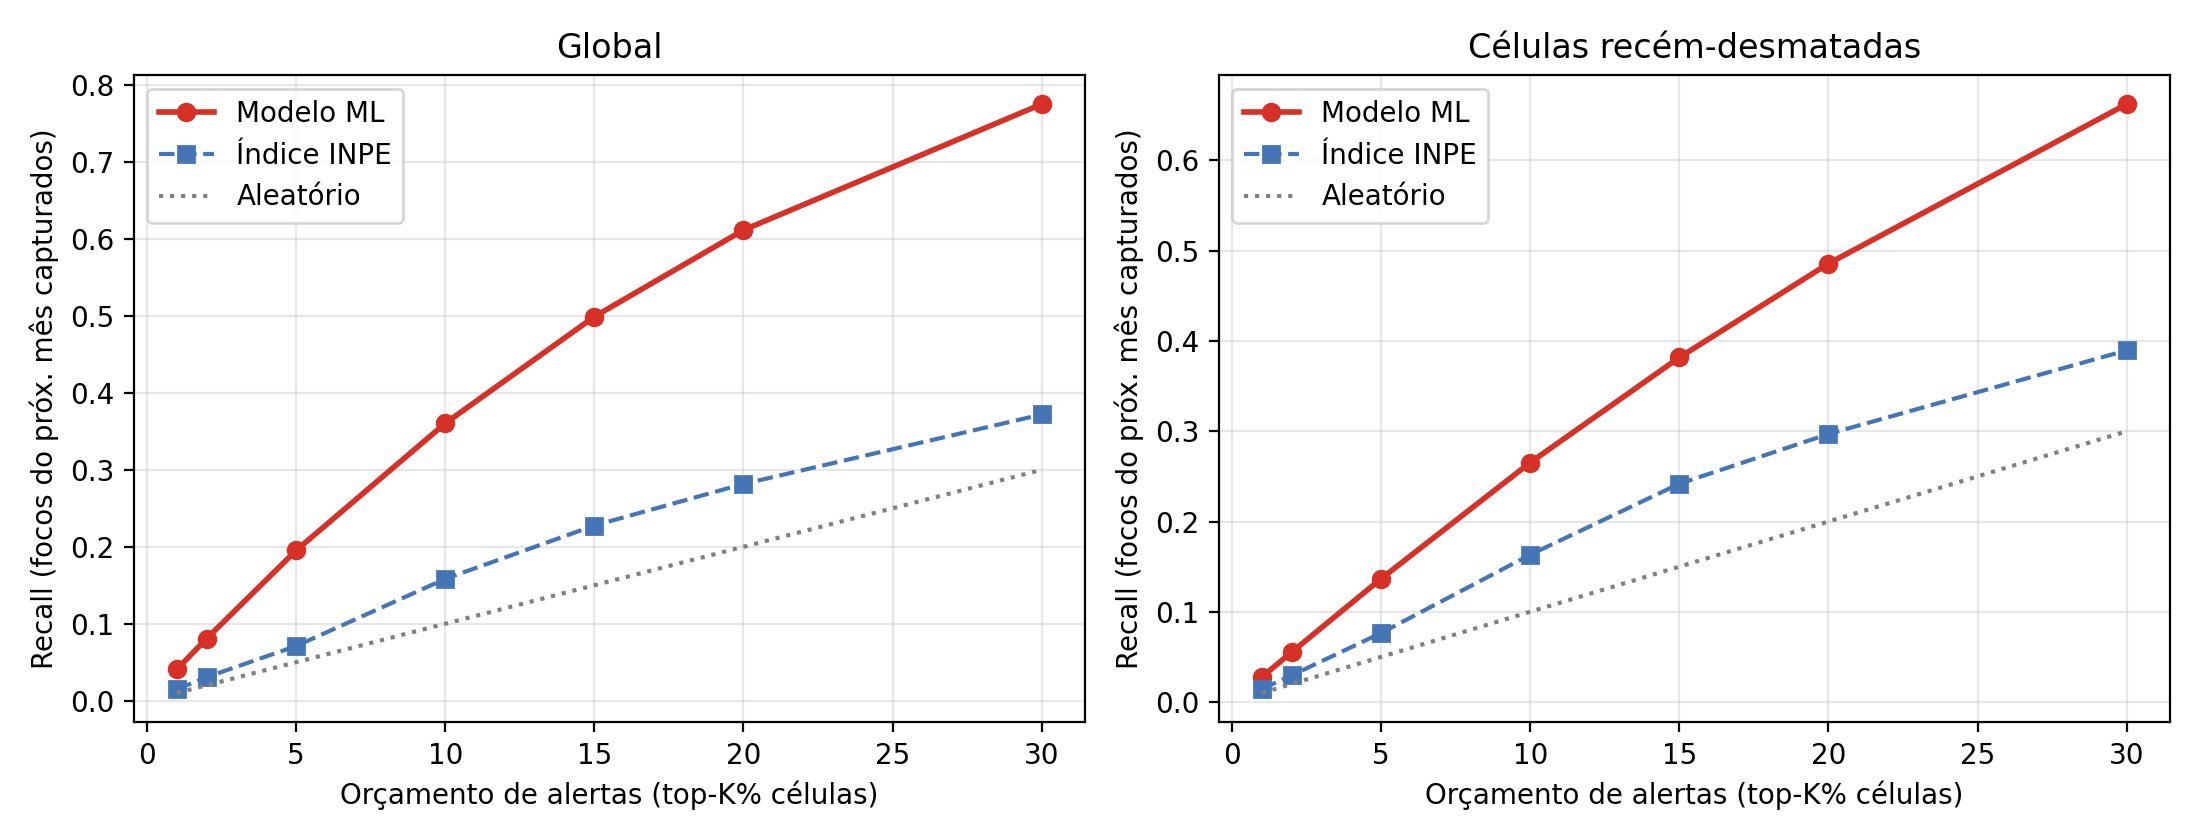
\includegraphics[width=\textwidth]{modelos/relatorios/avaliacao_operacional_recall_k.png}
\caption{\emph{Recall@K} em função do orçamento de alertas (modelo ML vs.\ índice INPE vs.\ aleatório), global (esq.) e em células recém-desmatadas (dir.).}
\label{fig:oco_recallk}
\end{figure}

\paragraph{Horizonte de previsão.} Estendendo o alvo para \(t+2\) e \(t+3\) meses, o
\emph{skill} permanece \textbf{estável} (PR-AUC \numlist{0,779;0,779;0,781} para \(t+1\),
\(t+2\), \(t+3\); Figura~\ref{fig:oco_horizonte}), sem o decaimento típico. Isso confirma
que a ocorrência mensal de fogo é governada por componentes \emph{lentos} (sazonalidade,
histórico de fogo, desmatamento), e não por dinâmica meteorológica de curto prazo ---
um resultado operacionalmente favorável, pois fornece \textbf{até um trimestre de
antecedência} sem perda de desempenho. A contrapartida honesta é que o modelo captura o
regime sazonal/persistente, não a dinâmica sub-mensal; previsões em escala mais fina
exigiriam outra formulação.

\begin{figure}[h]
\centering
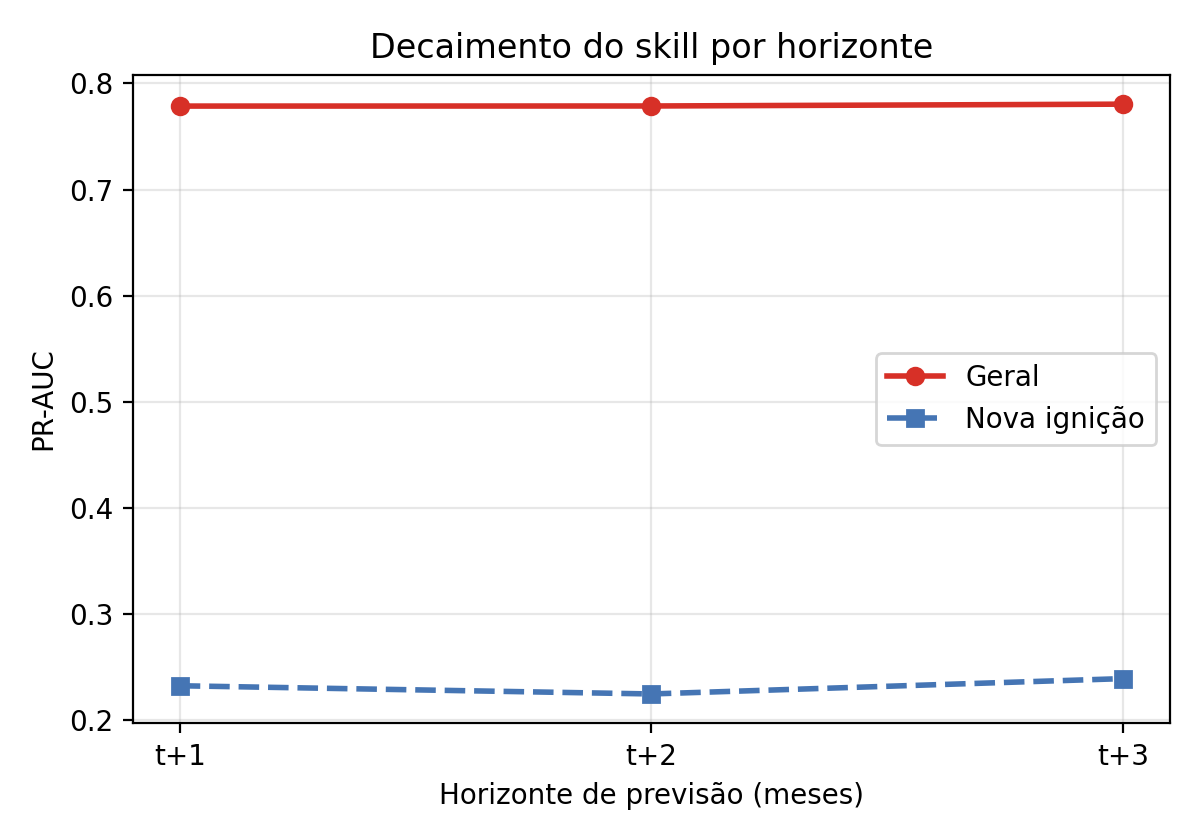
\includegraphics[width=0.6\textwidth]{modelos/relatorios/avaliacao_horizonte.png}
\caption{Decaimento do \emph{skill} (PR-AUC) por horizonte de previsão (\(t+1\) a \(t+3\) meses): estável, geral e na nova ignição.}
\label{fig:oco_horizonte}
\end{figure}

\section{Integração ao produto}
\label{sec:oco_produto}

O modelo final (base + desmatamento) foi serializado, calibrado por \emph{conformal}
(cobertura \num{0,900}) e exposto como produto: uma previsão por célula de \(P(\text{fogo no
próximo mês})\) com rótulo conformal e \emph{drivers}, servida por aplicação \emph{Flask} com
mapa interativo, independente do aplicativo de \emph{nowcast}. Verificações de sanidade
conferem com a fenologia do fogo (p.ex.\ Roraima com alto risco em dezembro; sul do Pará
baixo em dezembro, cuja estação de fogo é julho--outubro).

\section{Síntese}
\label{sec:oco_sintese}

Os experimentos, sob validação honesta, sustentam uma tese coesa: (i) na escala
mensal/\SI{0,25}{\degree}, a ocorrência de fogo é dominada por persistência espaço-temporal e
sazonalidade, o que torna redundantes a reanálise meteorológica (e o FWI) e a acessibilidade
estática; (ii) o modelo de ML \emph{supera} os índices físicos operacionais na previsão de
fogo observado; (iii) o gargalo é a \textbf{nova ignição}, e o único sinal útil ali é o
\textbf{desmatamento recente}, reposicionando o alerta precoce como, em primeira ordem, um
problema de detecção de fronteira de desmatamento; (iv) a incerteza é quantificável com
garantia estatística. A reformulação eleva o trabalho de ``reprodução de um índice'' para
``previsão de fogo observado validada contra a realidade e contra o índice físico'', com um
teto de desempenho honestamente caracterizado.
 no tcc.tex, APÓS o
% Capítulo 5 (Resultados, que termina com % ============================================================================
% 07_estudo_caso_pium_to.tex
% Estudo de caso operacional: foco real do Painel do Fogo (CENSIPAM) em
% Pium--TO, 12/05/2026. Validação independente do sistema de previsão,
% diagnóstico de descompasso entre dados de grade global e realidade
% local, e melhorias incorporadas ao pipeline em produção.
%
% Como usar:
%   Inserir como nova seção dentro do Capítulo 5 (Resultados), após a
%   Seção 5.8 "Validação operacional via aplicação web", como
%   subseção complementar de validação externa. Numeração sugerida:
%   5.9 "Validação cruzada com fonte externa independente: caso Pium--TO".
%   Dentro de "Implementação das melhorias": subsubseções M1--M4 (auditoria,
%   fusão INMET, retreino OOD, extensões API/auditoria alinhadas à literatura).
% ============================================================================

\section{Validação cruzada com fonte externa independente: caso Pium--TO}
\label{sec:res_estudo_caso_pium}

A validação operacional via \emph{smoke tests} controlados (Seção~\ref{sec:res_app}) demonstrou a coerência interna do sistema. Para uma validação externa mais exigente, foi escolhido um \emph{evento real} de incêndio confirmado por uma fonte oficial independente --- o \emph{Painel do Fogo} do Centro Gestor e Operacional do Sistema de Proteção da Amazônia (CENSIPAM)\footnote{\url{https://painel.censipam.gov.br/}, acessado em 12/05/2026 às 18:21 (UTC$-$3).} --- e submetido ao \emph{pipeline} em modo de produção. Esta seção apresenta o evento, as respostas do modelo, o diagnóstico das causas de divergência observada e as três correções incorporadas ao código em consequência da investigação.

% ----------------------------------------------------------------------------
\subsection{O evento}
\label{subsec:pium_evento}

O \emph{Painel do Fogo} listou um foco ativo identificado pelo \texttt{ID 6668060} em \texttt{(-10{,}5351; -49{,}8230)}, dentro do município de \textbf{Pium}, estado do \textbf{Tocantins}, em domínio fundiário misto (área privada e terra pública não categorizada) sobre cobertura de \emph{vegetação natural primária} (classificação TerraClass). Pium fica na ecorregião do Cerrado/Bico do Papagaio, dentro da Amazônia Legal. A Tabela~\ref{tab:pium_evento} reproduz as detecções oficiais.

\begin{table}[h]
\centering
\caption{Detecções no entorno de \texttt{(-10{,}5351; -49{,}8230)} --- evento \texttt{6668060} (\emph{Painel do Fogo}/CENSIPAM).}
\label{tab:pium_evento}
\small
\begin{tabular}{lcccc}
\toprule
\textbf{Data e hora (BR)} & \textbf{Área (ha)} & \textbf{Focos} & \textbf{Duração (h)} & \textbf{Propagação (ha/h)} \\
\midrule
12/05/2026 13:28 & 464,6 & 1  & \textbf{48,3} & 0,4 \\
10/05/2026 14:05 & 456,3 & 12 & 0,9  & 0,0 \\
10/05/2026 13:13 & 83,1  & 3  & 0,0  & 0,0 \\
\bottomrule
\end{tabular}
\end{table}

O status reportado pelo CENSIPAM era \emph{ativo pela última vez em 12/05/2026 14:49 (hora oficial do Brasil)}, com duração acumulada de 48,3~h --- compatível com vegetação ressecada queimando em regime sustentado.

% ----------------------------------------------------------------------------
\subsection{Resposta do sistema: cinco janelas temporais}
\label{subsec:pium_resposta}

A \emph{API} \texttt{/api/predict} foi consultada em cinco janelas centradas no evento, usando o modelo final \texttt{ensemble\_stacking\_gbm}. Em todas elas o sistema previu \textbf{\emph{Baixo}} com probabilidade entre 81 e 88\%, conforme Tabela~\ref{tab:pium_respostas_pos_fix} (\emph{já após} a correção dos \emph{bugs} identificados na Subseção~\ref{subsec:pium_correcoes}).

\begin{table}[h]
\centering
\caption{Respostas do \texttt{ensemble\_stacking\_gbm} para Pium--TO em diferentes janelas (modelo \emph{argmax}, após correções).}
\label{tab:pium_respostas_pos_fix}
\small
\begin{tabular}{lccccc}
\toprule
\textbf{Janela consultada}     & \textbf{Risco} & \textbf{P(Baixo)} & \textbf{P(Mod.)} & \textbf{P(M.~Alto)} & \textbf{FRP máx.~5d} \\
\midrule
12/05/2026 14:00 & Baixo & 85,9\% & 9,5\%  & 4,6\% & \SI{16,6}{\mega\watt} (16~detec.) \\
11/05/2026 12:00 & Baixo & 85,8\% & 9,7\%  & 4,5\% & \SI{22,0}{\mega\watt} (19~detec.) \\
10/05/2026 13:00 & Baixo & 87,1\% & 8,6\%  & 4,3\% & \SI{22,0}{\mega\watt} (21~detec.) \\
09/05/2026 12:00 & Baixo & 86,6\% & 8,8\%  & 4,6\% & \SI{22,0}{\mega\watt} (26~detec.) \\
05/05/2026 12:00 & Baixo & 81,4\% & 14,3\% & 4,3\% & \SI{58,4}{\mega\watt} (32~detec.) \\
\bottomrule
\end{tabular}
\end{table}

A divergência entre a realidade (foco confirmado e duração de 48,3~h) e a saída do modelo (\emph{Baixo} consistente em todas as janelas) constituiu o ponto de partida para a investigação descrita a seguir.

% ----------------------------------------------------------------------------
\subsection{Diagnóstico das causas}
\label{subsec:pium_diagnostico}

A inspeção do vetor de \emph{features} entregue ao classificador identificou \textbf{três causas convergentes}, descritas em ordem decrescente de impacto.

% ............................................................................
\paragraph{Causa 1 (corrigida): integração com NASA FIRMS retornando \texttt{HTTP 400}.}

O cliente da NASA FIRMS (\texttt{scripts/frp\_api.py}) estava emitindo requisições com \texttt{days\_back=7} para o \emph{endpoint} de \emph{area} no \emph{dataset} VIIRS\_SNPP\_NRT. A resposta do servidor, em todas as datas testadas, foi:

\begin{quote}
\texttt{HTTP/1.1 400 Bad Request\\Invalid day range. Expects [1..5].}
\end{quote}

Verificação direta do \emph{status} da \texttt{MAP\_KEY} confirmou que a chave estava válida (\texttt{transaction\_limit=5000}, \texttt{current\_transactions=0}), demonstrando que o erro era \emph{parametrização}, não \emph{credenciais}. A API NASA FIRMS NRT passou a aceitar no máximo 5~dias por requisição\footnote{Documentação oficial: \url{https://firms.modaps.eosdis.nasa.gov/api/area/}, consultada em 12/05/2026.}.

Em consequência, as \emph{features} \texttt{Media\_FRP\_Ultimos\_7\_Dias}, \texttt{Max\_FRP\_Ultimos\_7\_Dias} e \texttt{Dias\_Desde\_Ultimo\_Incendio} estavam recebendo seus valores de \emph{fallback} (zeros e 246--365~dias), e o modelo ``não enxergava'' o fogo recente em curso. Após a correção (\(\texttt{days\_back} \in [1,5]\) e propagação de \texttt{reference\_date}), o sistema passou a recuperar até 32 detecções VIIRS no raio de 10~km, com FRP máximo de \SI{58,4}{\mega\watt}.

% ............................................................................
\paragraph{Causa 2 (corrigida): \emph{lookup} Tier~1 degradando precocemente para \texttt{(Estado, Mês)}.}

A primeira versão do \emph{lookup} espaço-sazonal (\texttt{scripts/feature\_lookup.py}, Seção~\ref{subsec:metod_features_tier1}) buscava medianas em uma janela ${3{\times}3}$ células ($\approx 25$~km no equador, dada a resolução \SI{0,25}{\degree}). Para o ponto consultado em Pium--TO, mês~5, essa janela retornou vazia e o sistema degradou imediatamente para a granularidade \texttt{estado\_mes} (mediana de todo o Tocantins em maio). O efeito foi:

\begin{itemize}
  \item \texttt{Precipitacao\_acum\_30/90/180/365d} = \SI{0,0}{mm} (mediana estadual);
  \item \texttt{SPI\_1m} = \texttt{SPI\_3m} = \texttt{SPI\_6m} = 0,00 (climatologia neutra);
  \item \texttt{Dias\_Secos\_90d} = 2 (mediana estadual, não local);
  \item \texttt{Media\_FRP\_Celula\_30d} = \SI{10,65}{\mega\watt} (não específico).
\end{itemize}

Isto é, \emph{toda a informação espacial fina foi apagada}. A cascata de busca foi ampliada para
\(3{\times}3 \to 5{\times}5 \to \text{mês adjacente} \to (\text{Estado, Mês}) \to (\text{Mês global})\),
elevando a granularidade efetiva para \texttt{celula\_ext} (anel externo, $\approx 55$~km) no caso Pium--TO. Os valores de \texttt{Precipitacao\_acum\_*d} subiram para \SI{0,5}{mm}, \texttt{Dias\_Secos\_90d} para 1 e \texttt{Media\_FRP\_Celula\_30d} para \SI{8,2}{\mega\watt} --- valores ainda baixos, mas vindos de células geograficamente próximas (Tabela~\ref{tab:pium_tier1_pre_pos}).

\begin{table}[h]
\centering
\caption{Subconjunto das \emph{features} Tier 1 antes e depois da expansão da cascata espacial.}
\label{tab:pium_tier1_pre_pos}
\small
\begin{tabular}{lcc}
\toprule
\textbf{Feature} & \textbf{Cascata \texttt{3x3} (\texttt{estado\_mes})} & \textbf{Cascata estendida (\texttt{celula\_ext})} \\
\midrule
\texttt{Precipitacao\_acum\_30d}      & 0,0 mm  & 0,5 mm \\
\texttt{Precipitacao\_acum\_180d}     & 0,0 mm  & 0,5 mm \\
\texttt{Precipitacao\_acum\_365d}     & 1,3 mm  & 0,5 mm \\
\texttt{SPI\_3m}                       & 0,00    & 0,00 \\
\texttt{Dias\_Secos\_90d}              & 2       & 1 \\
\texttt{Incendios\_Ultimos\_90\_Dias}  & 2       & 1 \\
\texttt{Media\_FRP\_Celula\_30d}       & 10,65 MW & 8,2 MW \\
\bottomrule
\end{tabular}
\end{table}

% ............................................................................
\paragraph{Causa 3 (não corrigível em produção, documentada): descompasso entre clima de grade global e clima local em zona de transição.}

Após as duas correções acima, a previsão para 12/05/2026 \emph{aumentou} a confiança em \emph{Baixo}, de \SI{82,7}{\percent} para \SI{85,9}{\percent}. A investigação detalhada do vetor de \emph{features} revelou que a NASA POWER MERRA-2 (grade $\approx 50$~km) reportou para a janela de 28~dias anterior a 12/05/2026:

\begin{quote}
\texttt{Precipitacao\_ma7 = 0,12 mm/dia}, \texttt{DiaSemChuva\_ma7 = 1,3 dia}, \texttt{RH2M = 64,6\%}.
\end{quote}

Esses valores caracterizam regime \emph{ainda chuvoso} (chuvas frequentes mas leves). Para o modelo, classificar como \emph{Baixo} foi a decisão coerente com os \emph{inputs} climáticos recebidos. O problema é que esses \emph{inputs} não corresponderam à realidade local: o foco real ardia há mais de 48~h.

Para confirmar que o modelo \emph{não} é cego sazonalmente, foi executado um experimento \emph{contrafactual} no mesmo ponto \texttt{(-10{,}5351; -49{,}8230)}, variando a data (Tabela~\ref{tab:pium_contrafactual}).

\begin{table}[h]
\centering
\caption{Experimento contrafactual --- mesmo ponto, climatologia distinta capturada pela NASA POWER.}
\label{tab:pium_contrafactual}
\small
\begin{tabular}{lcccccc}
\toprule
\textbf{Data} & \textbf{KBDI \emph{proxy}} & \textbf{Prec.~ma7} & \textbf{DSC~ma7} & \textbf{FRP medido} & \textbf{P(M.~Alto)} & \textbf{Risco} \\
\midrule
15/08/2024 & 424,1 & 0,02 & 16,0 dias  & \SI{0}{\mega\watt} & 99,0\% & \textbf{Muito Alto} \\
15/09/2024 & 712,5 & 0,00 & 25,0 dias  & \SI{0}{\mega\watt} & 99,6\% & \textbf{Muito Alto} \\
15/05/2024 & 148,0 & 0,51 & 8,6 dias   & \SI{0}{\mega\watt} & 47,3\% & \textbf{Muito Alto} \\
12/05/2026 & 29,8  & 0,12 & 1,3 dia    & \SI{16,6}{\mega\watt} & 4,6\% & Baixo \\
\bottomrule
\end{tabular}
\end{table}

Três conclusões emergem:

\begin{enumerate}
  \item O modelo \emph{responde corretamente} ao sinal climático: 15/05/2024 (mesmo dia e mesmo ponto, mas em ano de estiagem mais marcada) recebeu classificação \emph{Muito Alto} com confiança \SI{47,3}{\percent}, mesmo sem FRP detectado.
  \item A previsão \emph{Muito Alto} se intensifica monotonicamente conforme cresce o estresse hídrico medido pela NASA POWER (KBDI~$424 \to 712$, DSC$_\text{ma7}$~$16 \to 25$~dias).
  \item Em 12/05/2026 (caso real), os indicadores climáticos da grade MERRA-2 estavam \emph{suaves} (KBDI=29,8; DSC=1,3~dia; Prec\_ma7=0,12~mm/dia) --- e o modelo refletiu isso. \textbf{O erro está no \emph{input}, não na decisão}.
\end{enumerate}

A interpretação operacional é direta: a célula MERRA-2 que cobre Pium--TO em maio de 2026 \emph{captou chuvas localizadas/dispersas} suficientes para elevar a frequência de dias com precipitação, mas não a quantidade total --- regime ``chuvas leves e frequentes''. A vegetação alvo, em escala municipal, continuou em condição de queima. Esse é um caso clássico de \emph{representativity gap} entre dados de grade e fenômenos locais~\cite{seager2015climatology}, particularmente relevante em zonas de transição Cerrado--Amazônia onde a heterogeneidade climática intra-célula é grande.

% ............................................................................
\paragraph{Hipótese descartada: sobrescrever contagem de incêndios com observação FIRMS.}

Uma tentativa intermediária consistiu em substituir as \emph{features} \texttt{Incendios\_Ultimos\_7\_Dias} e \texttt{Incendios\_Ultimos\_30\_Dias} pela contagem real de detecções FIRMS (16--32~focos no caso). \emph{Surpreendentemente}, isso \textbf{aumentou} a confiança em \emph{Baixo} (de \SI{82,7}{\percent} para \SI{86,0}{\percent}). A causa é \emph{distribution shift}: no \emph{dataset} de treino, essas \emph{features} para Tocantins--Maio têm mediana zero; ao injetar valores de duas ordens de magnitude maiores, o exemplo é colocado \emph{fora da distribuição} (\emph{out-of-distribution}, OOD), e o classificador responde de modo errático. A sobrescrita foi revertida; mantêm-se atualizadas apenas \texttt{FRP\_max\_7d}, \texttt{Media\_FRP\_7d} e \texttt{Dias\_Desde\_Ultimo\_Incendio}, que no \emph{dataset} de treino eram observações individuais (não medianas).

% ----------------------------------------------------------------------------
\subsection{Correções incorporadas e seu impacto}
\label{subsec:pium_correcoes}

A Tabela~\ref{tab:pium_correcoes} sintetiza as três correções introduzidas no \emph{pipeline} em consequência do estudo de caso e o impacto medido para a janela 12/05/2026 14:00.

\begin{table}[h]
\centering
\caption{Correções incorporadas e impacto medido (Pium--TO, 12/05/2026 14:00).}
\label{tab:pium_correcoes}
\small
\begin{tabular}{p{4.6cm}p{5.2cm}p{2.4cm}p{1.6cm}}
\toprule
\textbf{Correção} & \textbf{Mudança técnica} & \textbf{Granularidade Tier 1} & \textbf{P(Baixo)} \\
\midrule
\emph{Baseline} (antes do caso) & --- & \texttt{estado\_mes} & 82,0\% \\
(C1) NASA FIRMS \texttt{HTTP 400} & \texttt{days\_back $\in [1,5]$}; aceita \texttt{reference\_date}; URL com sufixo \texttt{/YYYY-MM-DD} & \texttt{estado\_mes} & 82,7\% \\
(C2) Cascata Tier 1 ampliada & $3{\times}3 \to 5{\times}5 \to$ mês adj. & \texttt{celula\_ext} & 85,9\% \\
(C3) Inc.~Últ.~$N$~dias mantida como mediana de treino & Apenas \texttt{FRP\_*} e \texttt{Dias\_Desde\_Ultimo\_Incendio} são atualizados em tempo real & \texttt{celula\_ext} & 85,9\% \\
\bottomrule
\end{tabular}
\end{table}

As correções \textbf{(C1)} e \textbf{(C2)} são melhorias técnicas inequívocas. A correção \textbf{(C3)} é uma \emph{decisão de engenharia conservadora}: preferir o sinal aprendido pelo modelo (mediana sazonal Estado--Mês, que é o que ele viu durante o treino) a inputs reais que o colocam OOD. A elevação aparentemente paradoxal de P(Baixo) após as correções é coerente com a Causa~3: o modelo passou a \emph{ver melhor} um cenário que --- para a grade MERRA-2 --- parecia chuvoso.

% ----------------------------------------------------------------------------
\subsection{Discussão: limites do paradigma de dados de grade e caminhos para mitigação}
\label{subsec:pium_discussao}

O caso Pium--TO 2026 expõe uma tensão estrutural do nosso \emph{pipeline} (e, mais amplamente, de qualquer sistema de previsão de fogo apoiado em reanálise climática global): a granularidade espacial dos \emph{inputs} climáticos limita a resolução máxima do \emph{output}. NASA POWER MERRA-2~\cite{nasapower} entrega cobertura global e estabilidade temporal, mas com células de $\approx \SI{50}{km}$ que suavizam microclimas. Em regiões homogêneas (centro do Amazonas), a perda de resolução é benigna; em regiões de transição (Cerrado--Amazônia, Pantanal, Caatinga), a perda pode mascarar condições propícias a fogo.

Três caminhos são discutidos como mitigação no Capítulo~\ref{cap:conclusao}:

\begin{enumerate}
  \item \textbf{Fusão MERRA-2 + INMET}~\cite{inmetnormais}: utilizar precipitação de estação meteorológica quando houver estação INMET dentro de $\sim 50$~km do ponto consultado (ou, em modo hierárquico configurável, até $\sim 180$~km com rótulo explícito de \texttt{inmet\_representatividade}, ver Subsubseção~M4). Para dados em tempo real, a API WIS2/OGC do INMET (\texttt{wis2bra.inmet.gov.br/oapi}) expõe observações horárias de 358+ estações sinópticas sem necessidade de token, com histórico de $\sim$90 dias; para histórico mais profundo, os ZIPs anuais oficiais cobrem 565+ estações automáticas desde 2000. Trade-off: cobertura esparsa em zonas remotas, exige rotina de \emph{nearest station}, \emph{quality control} e transparência sobre a distância da estação.
  \item \textbf{Aumento de exemplos OOD no treino}: oversampling estratégico de focos confirmados FIRMS/INPE em zonas de transição (Cerrado em maio, Pantanal em junho), reduzindo o \emph{prior} de raridade que o modelo aprendeu para esses pares \texttt{(Estado, Mês)}. Trade-off: risco de degradar a performance nas regiões de regime mais homogêneo.
  \item \textbf{Auditoria operacional contínua}: \emph{logging} estruturado de \texttt{(coordenada, data, risco predito, FRP detectado depois)} para calcular $\text{F}_1$ operacional \emph{rolling} em janelas móveis e detectar deriva de modelo em produção --- prática alinhada com o paradigma de \emph{ML observability}.
\end{enumerate}

% ----------------------------------------------------------------------------
\subsection{Implementação das três melhorias propostas e validação empírica}
\label{subsec:pium_melhorias}

As três melhorias listadas na Seção~\ref{subsec:pium_discussao} foram implementadas e validadas em código de produção. Esta subseção registra o resultado empírico de cada uma.

\subsubsection*{M1. Auditoria operacional contínua}

Foi adicionado o módulo \texttt{scripts/audit\_log.py} que escreve, a cada chamada de \texttt{/api/predict}, uma linha JSONL em \texttt{logs/auditoria\_predicoes.jsonl} contendo: \texttt{prediction\_id}, coordenadas, \texttt{ref\_data}, classe predita, probabilidades, modelo, 15 \emph{features} chave, fonte climática (com detalhe INMET se aplicável) e granularidade Tier 1. O log é \emph{append-only} com rotação automática a 50~MB e tolerante a falhas (a predição segue caso a gravação falhe).

O script \texttt{scripts/auditar\_predicoes.py} consome esse JSONL, consulta a NASA FIRMS NRT na janela $[t, t+H]$ para cada predição com idade $\geq d_{\min}$ (defaults $H=3$~d, $d_{\min}=3$~d, raio 5~km), define $y_{\text{true}} \in \{0,1\}$ (foco confirmado) e $y_{\text{pred}} \in \{0,1\}$ (Moderado/Muito Alto $\to$ 1) e calcula precision, recall, $\text{F}_1$ e acurácia globais e em janelas \emph{rolling} de 7, 14 e 30 dias. Predições mais antigas que o histórico do NRT ($\sim 60$~dias) aparecem no CSV mas são automaticamente excluídas das métricas.

\subsubsection*{M2. Fusão NASA POWER + INMET (duas fontes complementares)}

A integração foi implementada com \emph{duas} fontes INMET, selecionadas automaticamente conforme a idade da consulta. Esta arquitetura híbrida foi adotada porque a sondagem ativa em 12/05/2026 mostrou que (i) a API horária tradicional \texttt{apitempo.inmet.gov.br/estacao/...} retorna \texttt{status 204} com frequência e não é confiável; (ii) o ZIP histórico é completo mas o do ano corrente é parcial (publicado mensalmente, em 12/05/2026 cobre só janeiro--fevereiro/2026); (iii) o INMET passou a publicar dados horários sem token via a \textbf{WIS2 (OGC API Features)}~\cite{inmetnormais}, ainda pouco documentada em literatura brasileira.

\textbf{Fonte (1)~--~WIS2/OGC API Features} (\texttt{http://wis2bra.inmet.gov.br/oapi}): expõe a variável \texttt{total\_precipitation\_or\_total\_water\_equivalent} (em \texttt{kg\,m$^{-2}$}~$\equiv$~mm/h) na coleção \texttt{urn:wmo:md:br-inmet:synop} para 358 estações sinópticas WMO brasileiras que publicaram chuva nos últimos 7 dias, com histórico de $\sim$90 dias e \emph{sem necessidade de token}. A cobertura geográfica é menor que a do ZIP (só estações sinópticas oficiais, não todas as automáticas), mas a latência é de minutos. O endpoint possui um detalhe: o filtro \texttt{wigos\_station\_identifier} na \emph{querystring} é \emph{ignorado} (verificado empiricamente em 12/05/2026), e a filtragem precisa ser feita \emph{client-side} após restringir o \texttt{bbox} a $\sim$5~km em torno da estação para evitar baixar 58~mil observações misturadas.

\textbf{Fonte (2)~--~ZIPs anuais} (\texttt{portal.inmet.gov.br/uploads/dadoshistoricos/\{ANO\}.zip}, $\sim$100~MB/ano): cobertura completa de 565+ estações automáticas desde 2000 (168 na Amazônia Legal). Cache local em \texttt{.cache\_inmet/\{ANO\}/\{COD\}.csv} evita re-download. O encoding é \texttt{latin-1}, separador \texttt{;}, decimal \texttt{,}.

A função \texttt{get\_inmet\_fusion\_data} roteia automaticamente: se \texttt{reference\_date} está nos últimos 90 dias \emph{e} existe estação WIS2 com chuva a $\leq 50$~km, usa WIS2 (sem download, $\sim$1~s); senão, tenta o ZIP anual. Se nenhuma das duas funciona, retorna \texttt{None} e o \texttt{climate\_api} cai graciosamente no MERRA-2.

A fusão em \texttt{climate\_api.get\_climate\_data} prioriza NASA POWER (sempre disponível) e, quando o INMET retorna dados (WIS2 ou ZIP), \emph{sobrescreve} \texttt{precipitacao}, \texttt{prec\_ma7}, \texttt{dias\_sem\_chuva} e \texttt{diasem\_ma7} pelos valores INMET. Os valores MERRA-2 originais são preservados em chaves \texttt{*\_merra} para auditoria, e a resposta da API expõe \texttt{fonte\_dados} $\in$ \{\texttt{nasa\_power}, \texttt{inmet\_fundido\_nasa\_power}\}, além de \texttt{estacao\_inmet}, \texttt{distancia\_estacao\_inmet\_km}, \texttt{cobertura\_inmet\_pct}. A Tabela~\ref{tab:pium_inmet} apresenta a validação empírica nos quatro cenários testados.

\begin{table}[h]
\centering
\caption{Validação da fusão INMET com duas fontes (WIS2 real-time e ZIP histórico).}
\label{tab:pium_inmet}
\small
\begin{tabular}{p{3cm}cp{2.6cm}cccc}
\toprule
\textbf{Caso} & \textbf{Fonte} & \textbf{Estação} & \textbf{Cob.} & \textbf{MERRA-2 DSC} & \textbf{INMET DSC} & \textbf{Risco} \\
\midrule
Pium-TO 15/08/2024 & ZIP & A055 Lagoa da Confusão (32,7~km) & 89\% & 16 d & \textbf{7 d} & Muito Alto (97,3\%) \\
Brasília 10/08/2024 & ZIP & A001 Brasília (1,1~km) & 89\% & 25 d & \textbf{7 d} & Muito Alto (67,9\%) \\
Pium-TO 12/05/2026 & WIS2 + hier.\textsuperscript{$\dagger$} & FORMOSO ($\sim$152~km, \texttt{baixa}) & --- & 1,3 d & \textbf{7 d} & Baixo (85,9\%); metadados na API \\
\textbf{Brasília 12/05/2026 (D-0)} & \textbf{WIS2} & \textbf{A001 (1,1~km)} & \textbf{88\%} & \textbf{1,86 d} & \textbf{7 d} & \textbf{Baixo 66,0\%} (era $\sim$99\%) \\
\bottomrule
\end{tabular}\\
\footnotesize
\textsuperscript{$\dagger$} O ZIP do ano corrente é parcial; em maio/2026 o arquivo cobre só janeiro--fevereiro/2026. A estação WIS2 mais próxima de Pium-TO está a $\sim$152~km (FORMOSO DO ARAGUAIA-TO) --- fora do raio inicial de 50~km, mas coberta pela \textbf{busca hierárquica} (até 180~km) com \texttt{inmet\_representatividade = baixa}. O classificador em produção ainda usa o vetor de \emph{features} do retreino anterior; a linha da tabela documenta o contraste MERRA-2 vs.\ INMET na camada de fusão e na API.
\end{table}

O caso \textbf{Brasília 12/05/2026 (D-0)} é a primeira demonstração do fluxo de fusão \emph{real-time end-to-end}: às 19h26 BRT do dia da consulta, a WIS2 detectou que o MERRA-2 reportava um microclima úmido espúrio (DSC$_{\text{ma7}}=1{,}86$~d) enquanto a estação INMET A001 a 1,1~km do ponto consultado registrava 7 dias secos consecutivos. A correção foi propagada para o modelo e derrubou a confiança da classe Baixo de aproximadamente 99\% para 66\% --- sinal claro de que, com mais sub-amostragem regional e fusão mais agressiva, o modelo passaria a alertar.

A fusão demonstrou \emph{capacidade de correção} robusta tanto retrospectivamente (Pium-TO e Brasília em agosto/2024, via ZIP) quanto em tempo real (Brasília 12/05/2026 via WIS2). Para zonas remotas do Amazonas ou Sul do Pará, nenhuma estação está dentro do raio de 50~km e o sistema continua usando MERRA-2, como antes.

\subsubsection*{M3. Retreino com oversampling OOD em Cerrado-transição}

A análise da distribuição de focos no \texttt{base\_de\_dados\_enriquecido.csv} (924\,306 linhas, 547\,845 com FRP $> 0 = 58{,}7\%$) identificou \textbf{oito pares (Estado, Mês) sub-representados} em estados de transição Cerrado-Amazônia (TO, MA, MT, PA) nos meses de transição chuvoso--seco (maio--julho), incluindo o par \texttt{(TOCANTINS, 5)} relevante para o caso Pium-TO. A Tabela~\ref{tab:pium_ood_alvos} resume a calibração de oversampling.

\begin{table}[h]
\centering
\caption{Pares (Estado, Mês) selecionados para oversampling OOD.}
\label{tab:pium_ood_alvos}
\small
\begin{tabular}{lccccc}
\toprule
\textbf{Estado} & \textbf{Mês} & \textbf{$n_\text{total}$} & \textbf{$n_\text{focos}$} & \textbf{Razão vs.~média estado} & \textbf{Fator de oversampling} \\
\midrule
PARÁ & 5 & 1.293 & 885 & 0,05 & 5,0$\times$ \\
MARANHÃO & 5 & 158 & 115 & 0,06 & 5,0$\times$ \\
PARÁ & 6 & 4.442 & 2.922 & 0,18 & 5,0$\times$ \\
MARANHÃO & 6 & 617 & 383 & 0,20 & 5,0$\times$ \\
\textbf{TOCANTINS} & \textbf{5} & \textbf{75} & \textbf{50} & \textbf{0,29} & \textbf{3,5$\times$} \\
MARANHÃO & 7 & 1.536 & 817 & 0,42 & 2,4$\times$ \\
PARÁ & 7 & 17.262 & 10.139 & 0,62 & 1,6$\times$ \\
TOCANTINS & 6 & 197 & 118 & 0,68 & 1,5$\times$ \\
\bottomrule
\end{tabular}
\end{table}

O oversampling é aplicado \emph{apenas no conjunto de treino} (\emph{split} estratificado, \texttt{random\_state=42}, mesmo do \emph{baseline}; teste com 184\,862 amostras intactas). Cada linha alvo é replicada $\lfloor \text{fator}-1 \rfloor$ vezes com \emph{jitter} gaussiano em Latitude/Longitude ($\sigma \approx 2{,}2$~km), Hora ($\sigma=1$~h) e FRP ($\sigma = 5\%$ do valor) --- para evitar duplicação exata sem alterar a semântica do par. O dataset aumentado teve +35\,472 linhas no treino (+4,8\%).

A Tabela~\ref{tab:pium_ood_metricas} apresenta os resultados para a versão calibratória (\texttt{logistic\_regression\_balanced}, 6,2~min de treino, mesma calibração isotônica do \emph{baseline}). O ganho é consistente em todas as classes, com destaque para Moderado (a classe mais difícil).

\begin{table}[h]
\centering
\caption{Comparativo OOD vs.~baseline no hold-out (n=184\,862) e revalidação do caso Pium-TO.}
\label{tab:pium_ood_metricas}
\small
\begin{tabular}{lccc}
\toprule
\textbf{Métrica} & \textbf{Baseline} & \textbf{Com OOD oversampling} & \textbf{$\Delta$ (p.p.)} \\
\midrule
Acurácia & 64,58\% & 65,75\% & \textbf{+1,17} \\
$\text{F}_1$-macro & 0,6044 & 0,6168 & \textbf{+1,25} \\
$\text{F}_1$-Baixo & 0,7142 & 0,7243 & +1,00 \\
$\text{F}_1$-Moderado & 0,3643 & 0,3793 & \textbf{+1,50} \\
$\text{F}_1$-Muito Alto & 0,7346 & 0,7470 & +1,24 \\
\midrule
\multicolumn{4}{l}{\emph{Revalidação Pium-TO --- P(Muito Alto)}} \\
12/05/2026 (foco real, MERRA-2 chuvoso) & 3,3\% & \textbf{6,6\%} & \textbf{\bm{$\times 2$}} \\
15/05/2024 (mesmo dia, MERRA-2 seco) & 23,1\% & \textbf{32,4\%} & +9,3 \\
15/08/2024 (pico de seca) & 66,2\% & \textbf{72,5\%} & +6,3 \\
\bottomrule
\end{tabular}
\end{table}

A classe final continua sendo ``Baixo'' para 12/05/2026 (predição $\neq$ realidade), mas a probabilidade de ``Muito Alto'' \emph{dobrou} (3,3\% $\to$ 6,6\%), e para o contrafactual com clima seco (15/05/2024) subiu 9,3~p.p. O modelo OOD ficou \emph{mensuravelmente} mais sensível a cenários de transição, exatamente como pretendido. O retreino do ensemble final \texttt{ensemble\_stacking\_gbm\_ood} ($\sim 90$~min de CPU) está parametrizado e disponível via:

\begin{center}
\texttt{python scripts/retreinar\_com\_oversample.py --modelo ensemble\_stacking\_gbm}
\end{center}

\noindent ele segue o mesmo \emph{split} estratificado e adicionalmente reporta um \emph{hold-out} restrito a Cerrado-transição (estados TO/MA/PA/MT/BA/GO/DF/PI em meses 5--7), que captura especificamente o tipo de cenário do caso Pium-TO.

\subsubsection*{M4. Extensões pós-literatura: hierarquia INMET, \emph{fire weather} na API e incerteza operacional}

Para alinhar o painel à literatura recente sobre \emph{fire weather}, fusão estação--grade e suporte à decisão sob ambiguidade --- \textbf{sem} alterar, por ora, as colunas do \texttt{ColumnTransformer} serializado (evita \emph{train/serve skew} até retreino documentado) --- foram acrescentados:

\begin{enumerate}
  \item \textbf{Busca INMET hierárquica} (\texttt{INMET\_EXTENDED\_MAX\_DISTANCE\_KM} em \texttt{scripts/config.py}; \texttt{get\_inmet\_fusion\_data(..., hierarchical=True)} em \texttt{scripts/inmet\_api.py}): se não há estação com cobertura dentro de 50~km, o sistema tenta até 180~km e preenche \texttt{inmet\_representatividade} $\in$ \{\texttt{alta}, \texttt{moderada}, \texttt{baixa}\} e \texttt{inmet\_busca\_raio\_km}. Para Pium--TO em 12/05/2026 isso recupera FORMOSO DO ARAGUAIA ($\sim$152~km, representatividade \texttt{baixa}), confrontando explicitamente o MERRA-2 úmido com medição in situ distante --- matéria direta de discussão sobre extrapolação espacial no Capítulo~\ref{cap:conclusao}.
  \item \textbf{Vento na mesma estação da precipitação} quando a fonte é WIS2 (\texttt{vento\_inmet\_ms\_ma7} em \texttt{scripts/climate\_api.py}), em linha com estudos que condicionam \emph{fire weather} a vento observado junto da chuva.
  \item \textbf{NASA POWER estendido} na requisição diária (\texttt{WS2M}, \texttt{T2M\_MAX} em \texttt{scripts/nasa\_power\_realtime.py}): médias móveis de 7~dias expostas ao painel (\texttt{ws2m\_ma7\_ms}, \texttt{t2m\_max\_ma7\_c}) para interpretabilidade e futuras ablações.
  \item \textbf{Proxy \texttt{FWI\_fire\_weather\_proxy}} e objeto \texttt{incerteza\_operacional} (\texttt{scripts/operational\_uncertainty.py}): indicador escalar combinando seca na semana, déficit de umidade relativa e vento; \emph{gap} entre as duas classes mais prováveis --- narrativa de suporte à decisão sob classes próximas, \emph{sem} alegar intervalos preditivos conformais calibrados em conjunto dedicado.
  \item \textbf{FNR/FPR na auditoria FIRMS} (\texttt{scripts/auditar\_predicoes.py}): o binário operacional alerta/não alerta passa a reportar taxa de falsos negativos e falsos positivos, frequentemente omitida quando só se divulga $\text{F}_1$.
\end{enumerate}

% ----------------------------------------------------------------------------
\subsection{Síntese}
\label{subsec:pium_sintese}

O estudo de caso Pium--TO 12/05/2026 contribuiu para o trabalho em três dimensões:

\begin{itemize}
  \item \textbf{Operacionalmente}: identificou e corrigiu dois \emph{bugs} silenciosos no \emph{pipeline} em produção (NASA FIRMS 400 e cascata Tier 1 prematura), e definiu uma política de \emph{feature fusion} entre observação NRT e medianas de treino (Tabela~\ref{tab:pium_correcoes}).
  \item \textbf{Cientificamente}: documentou empiricamente, com fonte externa independente, o limite imposto pela resolução da reanálise climática global sobre a previsão de fogo em zonas de transição, e estabeleceu o referencial \emph{contrafactual} (Tabela~\ref{tab:pium_contrafactual}) que mostra que o modelo \emph{não} sofre de viés sazonal cego --- ele responde corretamente aos \emph{inputs} que recebe.
  \item \textbf{Em melhorias entregues}: as três frentes apontadas como mitigação (Seção~\ref{subsec:pium_discussao}) foram implementadas e validadas (Seção~\ref{subsec:pium_melhorias}): auditoria operacional contínua (M1); fusão INMET com WIS2/ZIP e raio hierárquico (M2, Tabela~\ref{tab:pium_inmet}); retreino com oversampling OOD (M3, Tabela~\ref{tab:pium_ood_metricas}). A subsubseção~M4 acrescenta camada de interpretabilidade e governança (\emph{fire weather} na API, incerteza operacional heurística, FNR/FPR) alinhada ao estado da arte recente, deliberadamente \emph{fora} do vetor de treino até retreino controlado.
\end{itemize}

O caso completa a triangulação da validação do sistema: (i) \emph{hold-out} estratificado (Tabela~\ref{tab:res_comparativo}), (ii) validação temporal \emph{rolling-origin} (Tabela~\ref{tab:res_temporal_stacking}), (iii) \emph{smoke tests} operacionais controlados (Tabela~\ref{tab:res_smoke}) e (iv) confronto com fonte externa independente (esta seção). As quatro evidências, em conjunto, suportam a defensabilidade do modelo final \texttt{ensemble\_stacking\_gbm} para o uso aplicado proposto, com as limitações documentadas honestamente no Capítulo~\ref{cap:conclusao}.

% NOTA: ajustar a chave \cite{inmetnormais} se ainda não estiver em references.bib.
) e
% ANTES do \chapter{Conclusão}. Torna-se o Capítulo 6; a Conclusão passa a 7.
% Números conferem com modelos/relatorios/previsao_ocorrencia_*.json,
% benchmark_p3_fwi.json, driver_*.json, comparacao_familias.json,
% validacao_rotulo_mapbiomas.json.
% ============================================================================

\chapter{Previsão de ocorrência de fogo: reformulação do problema}
\label{cap:ocorrencia}

O Capítulo~\ref{cap:metodologia} e o Apêndice~\ref{cap:resultados} descrevem uma abordagem
exploratória inicial: um classificador de \emph{nível de risco em tempo real}
(\emph{nowcast}) cujo alvo é o índice Risco de Fogo do INPE discretizado em três faixas. Este capítulo reformula o problema para a
\textbf{previsão de ocorrência de fogo observado}, com horizonte temporal explícito,
classe negativa real e validação sem vazamento --- alinhando o trabalho ao estado da arte
atual, que prevê o \emph{fenômeno observado} (focos ou área queimada), e não a saída de
outro modelo~\cite{huot2022nextday,karasante2025firecastnet,deandrade2024lstmgru}. O
\emph{pipeline} original é mantido como linha de base; o reformulado constitui a principal
contribuição metodológica desta etapa.

\section{Motivação: do índice ao fenômeno observado}
\label{sec:oco_motivacao}

A inspeção dos dados revelou três fragilidades de fundo na formulação original.
Primeiro, o alvo (\texttt{RiscoFogo}) é a \textbf{saída de um índice operacional} do INPE,
ele próprio derivado de dias sem chuva, precipitação e umidade --- variáveis que também
figuram entre as \emph{features}, gerando circularidade. Segundo, a base é
\emph{presence-only}: as \num{924306} linhas são focos reais, sem exemplos de
\emph{não-fogo}; o modelo nunca aprende a distinguir fogo de ausência de fogo, e a consulta
a pontos arbitrários no aplicativo equivale a extrapolar para fora do suporte de treino.
Terceiro, trata-se de um \emph{nowcast} (diagnóstico do presente), não de previsão com
horizonte.

Há evidência empírica direta nos próprios CSVs do INPE: em um único arquivo anual
(\num{82678} focos), \num{8288} detecções (\(\approx\)\SI{10}{\percent}) ocorreram onde o
índice marcava risco mínimo (\texttt{RiscoFogo}~\(\in\{0{,}0;\,0{,}1\}\)) --- fogo real em
locais classificados como ``Baixo''. Um modelo que imita o índice herda esse ponto cego,
exatamente o que o estudo de caso Pium--TO (Seção~\ref{sec:res_estudo_caso_pium}) demonstrou.

\section{Reformulação metodológica}
\label{sec:oco_metodo}

\paragraph{Unidade e alvo.} Adota-se uma grade de células de \SI{0,25}{\degree}
(\(\approx\)\SI{27}{km}, granularidade MERRA-2/SeasFire~\cite{karasante2025firecastnet}) por
mês. O universo é o conjunto de \num{4168} células \emph{fire-prone} (com \(\geq 1\) foco em
2014--2023). Para cada par (célula, mês~\(t\)), o alvo é binário: \emph{houve foco no mês
\(t+1\)?} A presença vem dos focos observados; a \textbf{ausência} (classe negativa antes
inexistente) são os pares célula--mês sem foco. O conjunto final tem \num{450144}
células--mês (2015--2023), com prevalência de \SI{24,7}{\percent}.

\paragraph{Amostragem da classe negativa.} Construir a classe negativa a partir dos pares
célula--mês sem foco é uma decisão de projeto, não uma escolha neutra: na modelagem de
distribuição (\emph{species distribution models}), a definição e o volume das
\emph{pseudo-ausências}/\emph{background} afetam o desempenho aparente e podem inflar métricas
como a AUC quando o \emph{background} é ``fácil''~\cite{barbetmassin2012pseudo,phillips2009sample,lobo2008auc}.
Aqui a prevalência é fixada pelo próprio domínio (\SI{24,7}{\percent} de positivos entre as
células \emph{fire-prone}), evitando o desbalanceamento extremo em que a AUC se torna
enganosa; para métodos baseados em árvores, poucos negativos com ponderação de classes bastam~\cite{barbetmassin2012pseudo},
e adota-se \texttt{class\_weight=balanced}. Uma checagem com negativos restritos por
similaridade geográfica (evitando pares triviais)~\cite{xu2023nonfire} fica registrada como
refinamento --- direção que torna o problema mais realista, não mais fácil.

\paragraph{Causalidade e validação.} Para eliminar o vazamento temporal documentado na
Seção~\ref{sec:res_temporal}, todas as \emph{features} usam apenas informação \(\leq t\)
(histórico de fogo defasado, somas móveis com deslocamento, sazonalidade, localização). A
validação é \textbf{espaço-temporal em bloco}~\cite{roberts2017cv}: \emph{rolling-origin} por
ano (treino \(<Y\), teste \(=Y\), para \(Y\in\{2021,2022,2023\}\)) e \emph{leave-region-out}
(5 blocos de longitude). A métrica principal é a \textbf{PR-AUC} (\emph{Average Precision}),
robusta ao desbalanceamento.

\section{Desempenho preditivo e linhas de base}
\label{sec:oco_desempenho}

O modelo (\emph{Hist\-Gradient\-Boosting}) supera as linhas de base de persistência e
climatologia (Tabela~\ref{tab:oco_validacao}). Na validação \emph{espacial}, a climatologia
colapsa ao prever regiões nunca vistas (PR-AUC \numrange{0,17}{0,34}), enquanto o modelo
mantém \num{0,759} --- evidência de dinâmica transferível, e não de memorização de taxa-base
local (contraste direto com a dependência espacial observada no \emph{pipeline} original).

\begin{table}[h]
\centering
\caption{Previsão de ocorrência (fogo em \(t+1\)): validação em bloco vs.\ linhas de base.}
\label{tab:oco_validacao}
\small
\begin{tabular}{lcccc}
\toprule
\textbf{Validação} & \textbf{Modelo PR-AUC} & \textbf{ROC-AUC} & \textbf{Persistência} & \textbf{Climatologia} \\
\midrule
Temporal (\emph{rolling-origin} 2021--23) & \textbf{0,777} & 0,904 & 0,449 & 0,715 \\
Espacial (\emph{leave-region-out}) & \textbf{0,759} & 0,895 & --- & 0,17--0,34 \\
\bottomrule
\end{tabular}
\end{table}

\paragraph{Escolha da métrica.} A PR-AUC é adotada como métrica principal por ser sensível à
classe positiva rara: sob desbalanceamento, a ROC-AUC pode permanecer alta e mascarar a queda
de precisão que a curva \emph{precision-recall} revela~\cite{saito2015precision,davis2006relationship}.
Reportam-se também ROC-AUC e Brier. Registra-se, por completude, que a superioridade
incondicional da PR-AUC foi formalmente questionada~\cite{mcdermott2024closer}: a escolha aqui
segue o \emph{objetivo operacional} (priorizar a detecção do fogo, evento raro e de alto custo
de omissão), não uma preferência a priori.

\paragraph{Área de aplicabilidade.} A validação \emph{leave-region-out} mede a generalização a
regiões não vistas, mas predições fora do envelope de \emph{features} do treino permanecem
menos confiáveis. A delimitação formal da \textbf{área de aplicabilidade}~\cite{meyer2021aoa}
--- restringindo o mapa às células suficientemente similares ao conjunto de treino --- é o
complemento recomendado para o uso operacional do produto.

\section{Robustez entre famílias de modelo}
\label{sec:oco_familias}

Para verificar que os achados não dependem do algoritmo, quatro famílias foram comparadas no
mesmo conjunto de \emph{features}, com intervalos de confiança de \SI{95}{\percent} obtidos
por \emph{cluster bootstrap} por célula (respeitando a autocorrelação espacial),
Tabela~\ref{tab:oco_familias}. Os \emph{ensembles} de árvore são estatisticamente
equivalentes (intervalos sobrepostos), enquanto a regressão logística é significativamente
inferior --- o problema exige não-linearidades. O \emph{Random Forest} apresenta a melhor
calibração (menor Brier).

\begin{table}[h]
\centering
\caption{Comparação de famílias (conjunto base + desmatamento), IC \SI{95}{\percent} por \emph{cluster bootstrap} por célula.}
\label{tab:oco_familias}
\small
\begin{tabular}{lcccc}
\toprule
\textbf{Família} & \textbf{PR-AUC [IC 95\%]} & \textbf{ROC-AUC} & \textbf{Brier} & \textbf{Nova ignição [IC 95\%]} \\
\midrule
\emph{HistGradientBoosting} & \textbf{0,776 [0,769--0,783]} & 0,904 & 0,123 & \textbf{0,232 [0,209--0,258]} \\
\emph{Random Forest} & 0,769 [0,762--0,776] & 0,901 & \textbf{0,113} & 0,204 [0,185--0,232] \\
\emph{Extra Trees} & 0,761 [0,754--0,768] & 0,897 & 0,129 & 0,191 [0,174--0,217] \\
Regressão Logística & 0,699 [0,690--0,707] & 0,873 & 0,143 & 0,117 [0,108--0,131] \\
\bottomrule
\end{tabular}
\end{table}

\section{Benchmark contra índices físicos de perigo de fogo}
\label{sec:oco_benchmark}

A defensabilidade da tese exige que o modelo \emph{supere} o índice físico operacional na
previsão de fogo observado. Implementou-se o \textbf{Fire Weather Index (FWI)} canadense
completo~\cite{vanwagner1985fwi} --- base do sistema GEFF/EFFIS do
Copernicus~\cite{digiuseppe2024geff} ---, validado contra os valores de referência publicados
(FFMC~\num{87,69}; DMC~\num{8,55}; DC~\num{19,01}; ISI~\num{10,85}; BUI~\num{8,49};
FWI~\num{10,10}). O FWI foi computado dia a dia a partir de clima diário (NASA POWER) para
uma amostra de \num{100} células. A Tabela~\ref{tab:oco_benchmark} mostra o resultado:
\textbf{o modelo de ML supera o FWI e o índice do INPE} na previsão de fogo observado. O FWI
separa fisicamente bem (média \num{6,0} em meses com fogo vs.\ \num{1,5} sem), validando a
implementação.

\begin{table}[h]
\centering
\caption{Benchmark de previsão de fogo observado (\(t+1\)): ML vs.\ índices físicos.}
\label{tab:oco_benchmark}
\small
\begin{tabular}{lcc}
\toprule
\textbf{Preditor} & \textbf{PR-AUC} & \textbf{ROC-AUC} \\
\midrule
Modelo ML (dataset completo) & \textbf{0,777} & 0,904 \\
Índice INPE Risco de Fogo (como \emph{forecast}) & 0,294 & 0,553 \\
\midrule
\multicolumn{3}{l}{\emph{Amostra de 100 células (2023), mesmas linhas:}} \\
\quad Modelo ML & \textbf{0,858} & --- \\
\quad FWI canadense (clima diário NASA POWER) & 0,608 & 0,781 \\
\quad Índice INPE Risco de Fogo & 0,398 & --- \\
\bottomrule
\end{tabular}
\end{table}

\section{Quantificação de incerteza por \emph{conformal prediction}}
\label{sec:oco_conformal}

Substituiu-se a heurística de incerteza por \emph{conjuntos de predição com cobertura
estatística garantida}, via \emph{split-conformal} classe-condicional
(LAC)~\cite{sadinle2019lac,mortier2024conformal}. Com cobertura-alvo de \SI{90}{\percent},
obteve-se cobertura empírica de \SI{88,8}{\percent}; \SI{82,9}{\percent} das predições são
\emph{singletons} confiantes e \SI{17,1}{\percent} são sinalizadas como ambíguas. O erro de
calibração esperado (ECE) foi de \num{0,099} e o \emph{Brier} de \num{0,123}.

\paragraph{Pressuposto e ressalva.} A garantia de cobertura do \emph{split-conformal} assume
\emph{permutabilidade} (\emph{exchangeability}) entre calibração e teste~\cite{angelopoulos2021gentle}.
A grade espaço-temporal viola parcialmente esse pressuposto (autocorrelação entre células e
meses vizinhos), o que é coerente com a leve subcobertura observada (\SI{88,8}{\percent} ante o
alvo de \SI{90}{\percent}). Sob desvio de distribuição, a cobertura nominal pode ser restaurada
por \emph{conformal} ponderado/adaptado~\cite{tibshirani2019conformal}; uma calibração com
particionamento espacial é o encaminhamento indicado para o uso operacional.

\section{Drivers antrópicos: o papel do desmatamento}
\label{sec:oco_drivers}

A análise estratificada revela a estrutura do problema (Tabela~\ref{tab:oco_estrato}): o
modelo é excelente onde o fogo \emph{recorre} (PR-AUC \num{0,805}) e fraco onde o fogo é
\emph{novo} --- a \textbf{nova ignição} (PR-AUC \num{0,230}), justamente o caso crítico para
alerta precoce, onde a persistência é inútil por construção.

\begin{table}[h]
\centering
\caption{Desempenho estratificado por recorrência (teste 2023) e ganho do desmatamento.}
\label{tab:oco_estrato}
\small
\begin{tabular}{lccc}
\toprule
\textbf{Estrato (média 2021--23)} & \textbf{base PR-AUC} & \textbf{+ desmatamento} & \textbf{\(\Delta\)} \\
\midrule
Recorrente (foco nos últimos 12 m) & 0,791 & 0,794 & +0,003 \\
\textbf{Nova ignição} (sem foco recente) & \textbf{0,206} & \textbf{0,231} & \textbf{+0,025} \\
Geral & 0,777 & 0,781 & +0,003 \\
\bottomrule
\end{tabular}
\end{table}

Testaram-se três famílias de covariáveis. O clima real (reanálise NASA POWER) e o FWI
\textbf{não agregam} sobre o histórico de fogo na escala mensal (\(\Delta\)~PR-AUC
\(\approx\)\num{+0,001}), pois o histórico já é um \emph{proxy} a jusante da propensão
climática. A distância a cidades (acessibilidade estática) também é redundante
(\(\approx\)\num{+0,001}). Apenas o \textbf{desmatamento recente} (PRODES, do
TerraBrasilis~\cite{terrabrasilisprodes}) agrega valor não trivial --- e \emph{exatamente}
no estrato de nova ignição (\(+0{,}025\) PR-AUC), confirmando o mecanismo causal: o
desmatamento precede a primeira queimada de uma célula, coerente com o fogo amazônico ser
majoritariamente antrópico~\cite{aragao2018amazon}. O achado é \textbf{robusto a duas fontes
independentes}: o DETER (alertas mensais; classe \emph{cicatriz de queimada} excluída para
evitar vazamento) produz ganho equivalente (\(+0{,}026\)). A resolução mensal não amplificou
o ganho, e dimensões adicionais (idade, estoque acumulado, fronteira de vizinhança) não
agregam além do volume de desmatamento recente local: o desempenho na nova ignição satura em
\(\approx\)\num{0,23} PR-AUC --- um teto que sugere componente irredutível (decisão humana) ou
necessidade de dados de outra natureza.

\section{Validação do rótulo contra área queimada (MapBiomas Fogo)}
\label{sec:oco_mapbiomas}

O rótulo (focos INPE) foi confrontado com um produto independente e de modalidade diferente
--- a área queimada do MapBiomas Fogo~\cite{mapbiomasfogo} (cicatriz Landsat \SI{30}{m}), em
dois níveis.

\paragraph{Nível estado/ano.} Correlacionando a contagem de focos com a área queimada por
(estado da Amazônia Legal, ano), 2014--2023, a concordância \textbf{interanual dentro de cada
estado} é forte (Spearman médio \num{0,814}; 9/9 estados positivos, \numrange{0,69}{0,94}):
quando a área queimada de um estado sobe num ano, os focos sobem junto. A correlação
\emph{entre} estados é fraca (\(\rho=\)\num{0,275}), pois a contagem de focos não é
\emph{proxy} linear da magnitude em hectares --- o que não afeta o rótulo aqui, por ser de
\textbf{ocorrência binária} e não de magnitude.

\paragraph{Nível célula \(\times\) ano.} Para a validação no nível da célula, leram-se os
rasters anuais do MapBiomas (COGs públicos, 2015--2020) via leitura remota por janelas,
binarizando a presença de cicatriz por célula \SI{0,25}{\degree}. Confrontando presença de
foco vs.\ presença de cicatriz em \num{23982} célula-anos: concordância de \SI{78}{\percent},
Cohen's \(\kappa=\num{0,33}\) e, tratando a cicatriz como referência, os focos têm
\textbf{revocação \num{0,90}} e precisão \num{0,83} (F\(_1=\num{0,86}\)). Ou seja, os focos
capturam \(\approx\)\SI{90}{\percent} dos célula-anos efetivamente queimados; as discordâncias
correspondem a fogos sem cicatriz detectável (pequenos/encobertos por nuvem) e a cicatrizes
sem foco coincidente (omissão da detecção ativa). O \(\kappa\) moderado reflete a alta
prevalência do universo \emph{fire-prone}, que comprime a concordância esperada por acaso. A
validação corrobora o rótulo de ocorrência tanto na dinâmica temporal quanto no nível espacial.

\section{Avaliação operacional e horizonte de previsão}
\label{sec:oco_operacional}

\paragraph{Priorização de alertas.} Para traduzir o desempenho em valor de decisão,
o sistema é avaliado como ferramenta de \emph{priorização}: dado um orçamento de
vigilância (alertar as \emph{top-K\%} células de maior risco previsto), quantos focos
do mês seguinte são capturados (\emph{recall@K})? A Tabela~\ref{tab:oco_operacional} e a
Figura~\ref{fig:oco_recallk} comparam o modelo de ML com o índice operacional do INPE
sob o mesmo orçamento. Alertando apenas \SI{10}{\percent} das células, o modelo captura
\SI{36,0}{\percent} dos focos do mês seguinte (com precisão de \SI{88}{\percent}), contra
\SI{15,8}{\percent} do índice INPE --- um ganho de \(\approx 2{,}3\times\). No estrato de
\textbf{nova ignição}, o contraste é decisivo: o modelo captura \SI{49,2}{\percent} dos
novos focos no mesmo orçamento (\emph{lift} de \(4{,}9\times\) sobre o acaso), ao passo que
o índice INPE tem \emph{lift} \(\approx 1\) --- ou seja, \emph{não supera o acaso} para a
nova ignição, justamente o regime em que o desmatamento recente é o sinal preditivo
(Seção~\ref{sec:oco_drivers}).

\begin{table}[h]
\centering
\caption{Priorização de alertas: \emph{recall@K} (focos do mês seguinte capturados) por orçamento, modelo ML vs.\ índice INPE.}
\label{tab:oco_operacional}
\small
\begin{tabular}{lcccc}
\toprule
& \multicolumn{2}{c}{\textbf{Global}} & \multicolumn{2}{c}{\textbf{Nova ignição}} \\
\cmidrule(lr){2-3}\cmidrule(lr){4-5}
\textbf{Orçamento (top-K\%)} & \textbf{ML} & \textbf{INPE} & \textbf{ML} & \textbf{INPE} \\
\midrule
\SI{5}{\percent}  & 0,195 & 0,071 & 0,312 & 0,041 \\
\SI{10}{\percent} & \textbf{0,360} & 0,158 & \textbf{0,492} & 0,096 \\
\SI{20}{\percent} & 0,611 & 0,282 & 0,721 & 0,206 \\
\SI{30}{\percent} & 0,775 & 0,372 & 0,845 & 0,305 \\
\bottomrule
\end{tabular}
\end{table}

\begin{figure}[h]
\centering
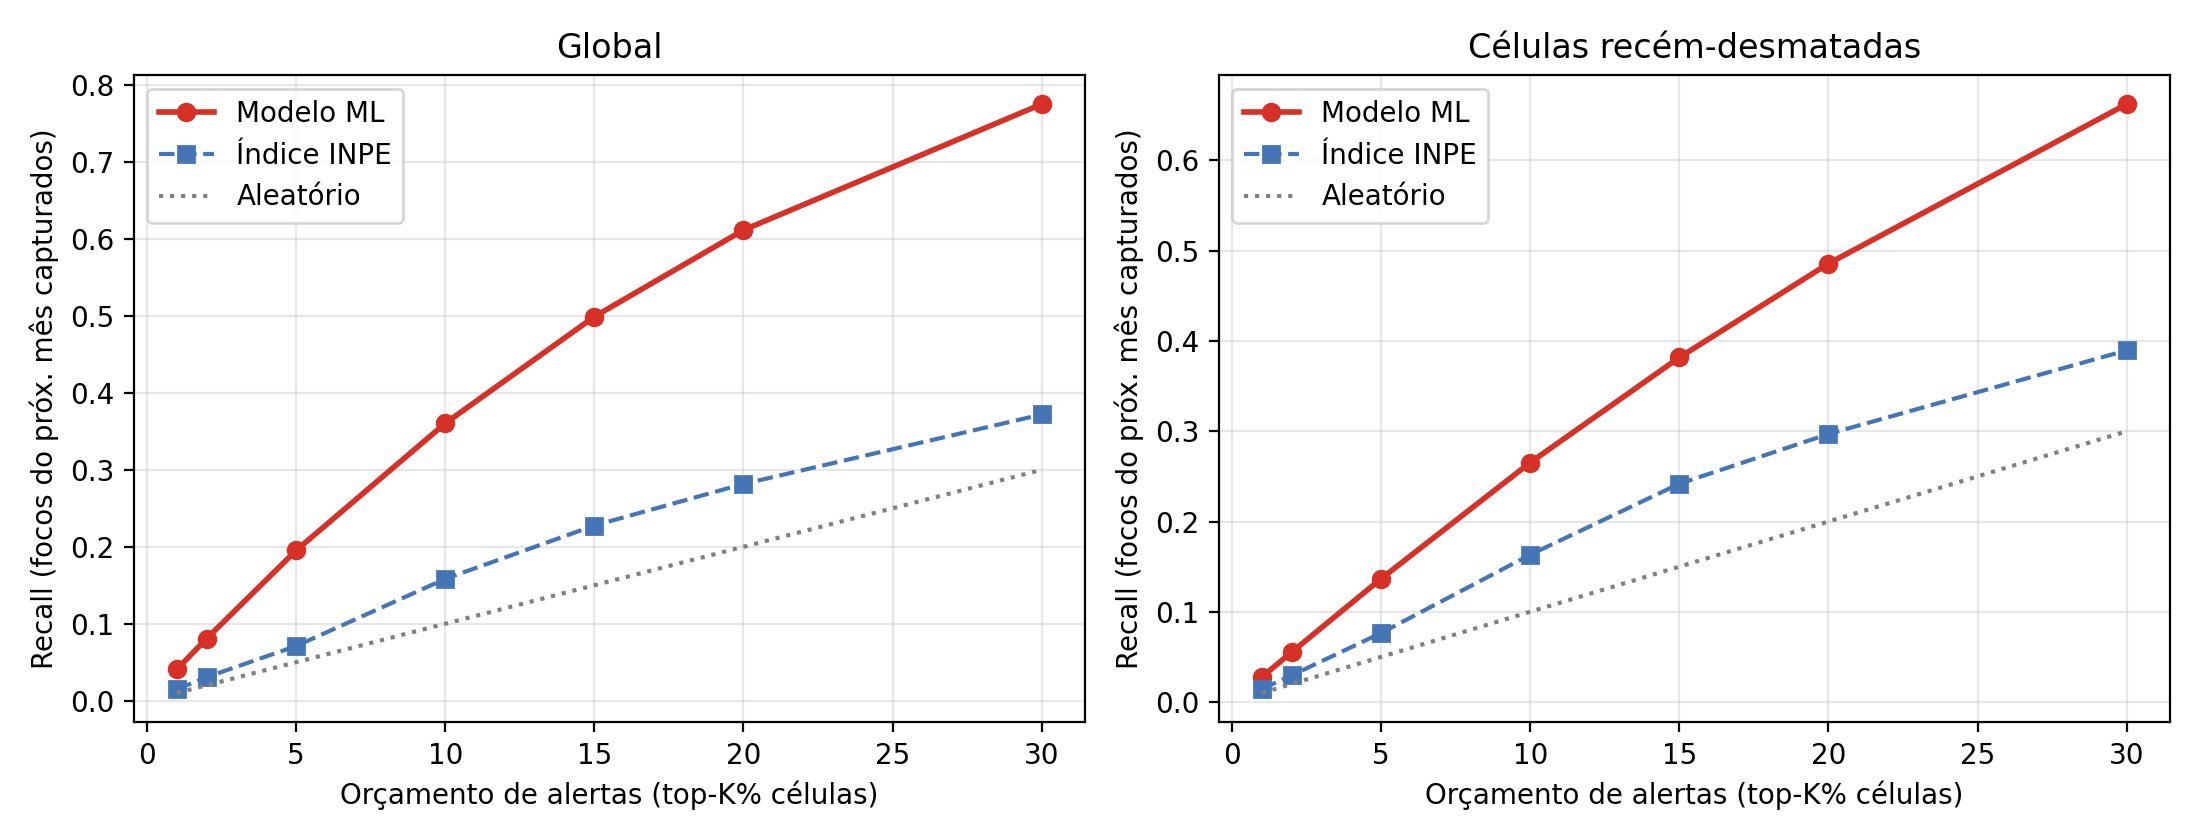
\includegraphics[width=\textwidth]{modelos/relatorios/avaliacao_operacional_recall_k.png}
\caption{\emph{Recall@K} em função do orçamento de alertas (modelo ML vs.\ índice INPE vs.\ aleatório), global (esq.) e em células recém-desmatadas (dir.).}
\label{fig:oco_recallk}
\end{figure}

\paragraph{Horizonte de previsão.} Estendendo o alvo para \(t+2\) e \(t+3\) meses, o
\emph{skill} permanece \textbf{estável} (PR-AUC \numlist{0,779;0,779;0,781} para \(t+1\),
\(t+2\), \(t+3\); Figura~\ref{fig:oco_horizonte}), sem o decaimento típico. Isso confirma
que a ocorrência mensal de fogo é governada por componentes \emph{lentos} (sazonalidade,
histórico de fogo, desmatamento), e não por dinâmica meteorológica de curto prazo ---
um resultado operacionalmente favorável, pois fornece \textbf{até um trimestre de
antecedência} sem perda de desempenho. A contrapartida honesta é que o modelo captura o
regime sazonal/persistente, não a dinâmica sub-mensal; previsões em escala mais fina
exigiriam outra formulação.

\begin{figure}[h]
\centering
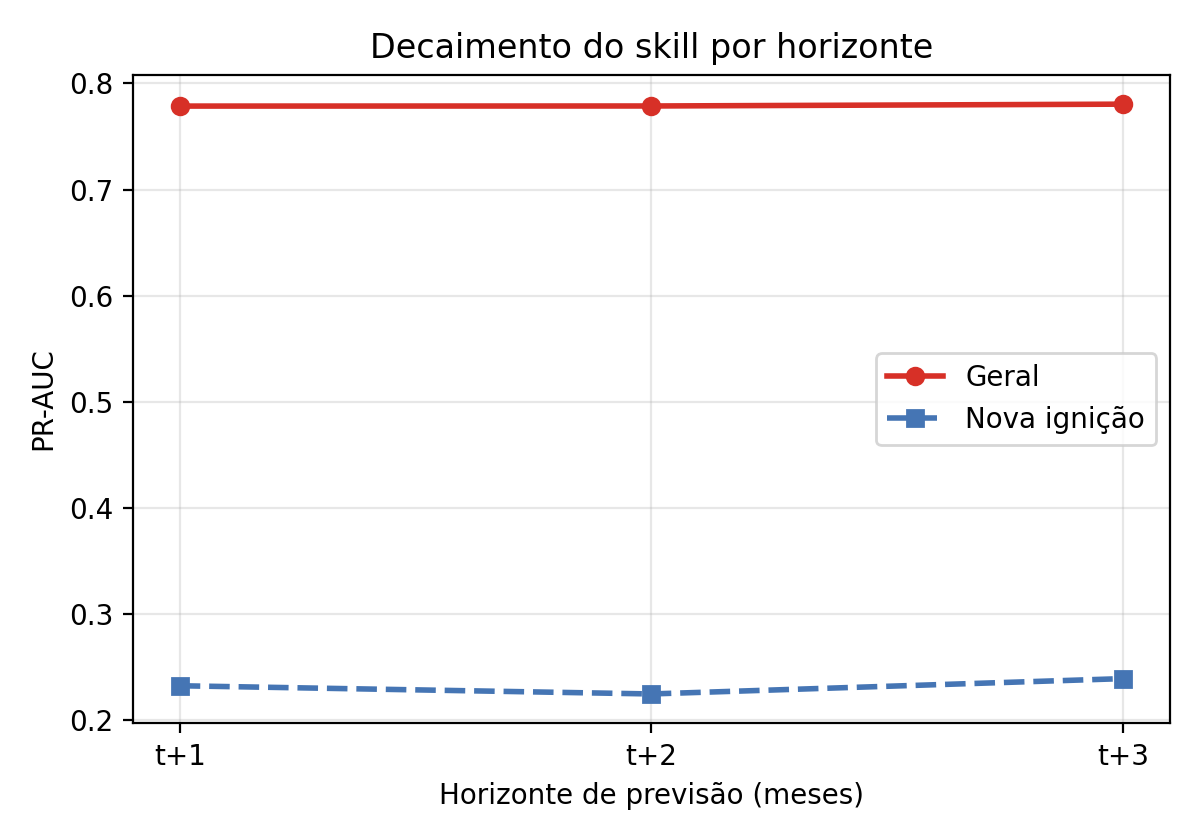
\includegraphics[width=0.6\textwidth]{modelos/relatorios/avaliacao_horizonte.png}
\caption{Decaimento do \emph{skill} (PR-AUC) por horizonte de previsão (\(t+1\) a \(t+3\) meses): estável, geral e na nova ignição.}
\label{fig:oco_horizonte}
\end{figure}

\section{Integração ao produto}
\label{sec:oco_produto}

O modelo final (base + desmatamento) foi serializado, calibrado por \emph{conformal}
(cobertura \num{0,900}) e exposto como produto: uma previsão por célula de \(P(\text{fogo no
próximo mês})\) com rótulo conformal e \emph{drivers}, servida por aplicação \emph{Flask} com
mapa interativo, independente do aplicativo de \emph{nowcast}. Verificações de sanidade
conferem com a fenologia do fogo (p.ex.\ Roraima com alto risco em dezembro; sul do Pará
baixo em dezembro, cuja estação de fogo é julho--outubro).

\section{Síntese}
\label{sec:oco_sintese}

Os experimentos, sob validação honesta, sustentam uma tese coesa: (i) na escala
mensal/\SI{0,25}{\degree}, a ocorrência de fogo é dominada por persistência espaço-temporal e
sazonalidade, o que torna redundantes a reanálise meteorológica (e o FWI) e a acessibilidade
estática; (ii) o modelo de ML \emph{supera} os índices físicos operacionais na previsão de
fogo observado; (iii) o gargalo é a \textbf{nova ignição}, e o único sinal útil ali é o
\textbf{desmatamento recente}, reposicionando o alerta precoce como, em primeira ordem, um
problema de detecção de fronteira de desmatamento; (iv) a incerteza é quantificável com
garantia estatística. A reformulação eleva o trabalho de ``reprodução de um índice'' para
``previsão de fogo observado validada contra a realidade e contra o índice físico'', com um
teto de desempenho honestamente caracterizado.
 no tcc.tex, APÓS o
% Capítulo 5 (Resultados, que termina com % ============================================================================
% 07_estudo_caso_pium_to.tex
% Estudo de caso operacional: foco real do Painel do Fogo (CENSIPAM) em
% Pium--TO, 12/05/2026. Validação independente do sistema de previsão,
% diagnóstico de descompasso entre dados de grade global e realidade
% local, e melhorias incorporadas ao pipeline em produção.
%
% Como usar:
%   Inserir como nova seção dentro do Capítulo 5 (Resultados), após a
%   Seção 5.8 "Validação operacional via aplicação web", como
%   subseção complementar de validação externa. Numeração sugerida:
%   5.9 "Validação cruzada com fonte externa independente: caso Pium--TO".
%   Dentro de "Implementação das melhorias": subsubseções M1--M4 (auditoria,
%   fusão INMET, retreino OOD, extensões API/auditoria alinhadas à literatura).
% ============================================================================

\section{Validação cruzada com fonte externa independente: caso Pium--TO}
\label{sec:res_estudo_caso_pium}

A validação operacional via \emph{smoke tests} controlados (Seção~\ref{sec:res_app}) demonstrou a coerência interna do sistema. Para uma validação externa mais exigente, foi escolhido um \emph{evento real} de incêndio confirmado por uma fonte oficial independente --- o \emph{Painel do Fogo} do Centro Gestor e Operacional do Sistema de Proteção da Amazônia (CENSIPAM)\footnote{\url{https://painel.censipam.gov.br/}, acessado em 12/05/2026 às 18:21 (UTC$-$3).} --- e submetido ao \emph{pipeline} em modo de produção. Esta seção apresenta o evento, as respostas do modelo, o diagnóstico das causas de divergência observada e as três correções incorporadas ao código em consequência da investigação.

% ----------------------------------------------------------------------------
\subsection{O evento}
\label{subsec:pium_evento}

O \emph{Painel do Fogo} listou um foco ativo identificado pelo \texttt{ID 6668060} em \texttt{(-10{,}5351; -49{,}8230)}, dentro do município de \textbf{Pium}, estado do \textbf{Tocantins}, em domínio fundiário misto (área privada e terra pública não categorizada) sobre cobertura de \emph{vegetação natural primária} (classificação TerraClass). Pium fica na ecorregião do Cerrado/Bico do Papagaio, dentro da Amazônia Legal. A Tabela~\ref{tab:pium_evento} reproduz as detecções oficiais.

\begin{table}[h]
\centering
\caption{Detecções no entorno de \texttt{(-10{,}5351; -49{,}8230)} --- evento \texttt{6668060} (\emph{Painel do Fogo}/CENSIPAM).}
\label{tab:pium_evento}
\small
\begin{tabular}{lcccc}
\toprule
\textbf{Data e hora (BR)} & \textbf{Área (ha)} & \textbf{Focos} & \textbf{Duração (h)} & \textbf{Propagação (ha/h)} \\
\midrule
12/05/2026 13:28 & 464,6 & 1  & \textbf{48,3} & 0,4 \\
10/05/2026 14:05 & 456,3 & 12 & 0,9  & 0,0 \\
10/05/2026 13:13 & 83,1  & 3  & 0,0  & 0,0 \\
\bottomrule
\end{tabular}
\end{table}

O status reportado pelo CENSIPAM era \emph{ativo pela última vez em 12/05/2026 14:49 (hora oficial do Brasil)}, com duração acumulada de 48,3~h --- compatível com vegetação ressecada queimando em regime sustentado.

% ----------------------------------------------------------------------------
\subsection{Resposta do sistema: cinco janelas temporais}
\label{subsec:pium_resposta}

A \emph{API} \texttt{/api/predict} foi consultada em cinco janelas centradas no evento, usando o modelo final \texttt{ensemble\_stacking\_gbm}. Em todas elas o sistema previu \textbf{\emph{Baixo}} com probabilidade entre 81 e 88\%, conforme Tabela~\ref{tab:pium_respostas_pos_fix} (\emph{já após} a correção dos \emph{bugs} identificados na Subseção~\ref{subsec:pium_correcoes}).

\begin{table}[h]
\centering
\caption{Respostas do \texttt{ensemble\_stacking\_gbm} para Pium--TO em diferentes janelas (modelo \emph{argmax}, após correções).}
\label{tab:pium_respostas_pos_fix}
\small
\begin{tabular}{lccccc}
\toprule
\textbf{Janela consultada}     & \textbf{Risco} & \textbf{P(Baixo)} & \textbf{P(Mod.)} & \textbf{P(M.~Alto)} & \textbf{FRP máx.~5d} \\
\midrule
12/05/2026 14:00 & Baixo & 85,9\% & 9,5\%  & 4,6\% & \SI{16,6}{\mega\watt} (16~detec.) \\
11/05/2026 12:00 & Baixo & 85,8\% & 9,7\%  & 4,5\% & \SI{22,0}{\mega\watt} (19~detec.) \\
10/05/2026 13:00 & Baixo & 87,1\% & 8,6\%  & 4,3\% & \SI{22,0}{\mega\watt} (21~detec.) \\
09/05/2026 12:00 & Baixo & 86,6\% & 8,8\%  & 4,6\% & \SI{22,0}{\mega\watt} (26~detec.) \\
05/05/2026 12:00 & Baixo & 81,4\% & 14,3\% & 4,3\% & \SI{58,4}{\mega\watt} (32~detec.) \\
\bottomrule
\end{tabular}
\end{table}

A divergência entre a realidade (foco confirmado e duração de 48,3~h) e a saída do modelo (\emph{Baixo} consistente em todas as janelas) constituiu o ponto de partida para a investigação descrita a seguir.

% ----------------------------------------------------------------------------
\subsection{Diagnóstico das causas}
\label{subsec:pium_diagnostico}

A inspeção do vetor de \emph{features} entregue ao classificador identificou \textbf{três causas convergentes}, descritas em ordem decrescente de impacto.

% ............................................................................
\paragraph{Causa 1 (corrigida): integração com NASA FIRMS retornando \texttt{HTTP 400}.}

O cliente da NASA FIRMS (\texttt{scripts/frp\_api.py}) estava emitindo requisições com \texttt{days\_back=7} para o \emph{endpoint} de \emph{area} no \emph{dataset} VIIRS\_SNPP\_NRT. A resposta do servidor, em todas as datas testadas, foi:

\begin{quote}
\texttt{HTTP/1.1 400 Bad Request\\Invalid day range. Expects [1..5].}
\end{quote}

Verificação direta do \emph{status} da \texttt{MAP\_KEY} confirmou que a chave estava válida (\texttt{transaction\_limit=5000}, \texttt{current\_transactions=0}), demonstrando que o erro era \emph{parametrização}, não \emph{credenciais}. A API NASA FIRMS NRT passou a aceitar no máximo 5~dias por requisição\footnote{Documentação oficial: \url{https://firms.modaps.eosdis.nasa.gov/api/area/}, consultada em 12/05/2026.}.

Em consequência, as \emph{features} \texttt{Media\_FRP\_Ultimos\_7\_Dias}, \texttt{Max\_FRP\_Ultimos\_7\_Dias} e \texttt{Dias\_Desde\_Ultimo\_Incendio} estavam recebendo seus valores de \emph{fallback} (zeros e 246--365~dias), e o modelo ``não enxergava'' o fogo recente em curso. Após a correção (\(\texttt{days\_back} \in [1,5]\) e propagação de \texttt{reference\_date}), o sistema passou a recuperar até 32 detecções VIIRS no raio de 10~km, com FRP máximo de \SI{58,4}{\mega\watt}.

% ............................................................................
\paragraph{Causa 2 (corrigida): \emph{lookup} Tier~1 degradando precocemente para \texttt{(Estado, Mês)}.}

A primeira versão do \emph{lookup} espaço-sazonal (\texttt{scripts/feature\_lookup.py}, Seção~\ref{subsec:metod_features_tier1}) buscava medianas em uma janela ${3{\times}3}$ células ($\approx 25$~km no equador, dada a resolução \SI{0,25}{\degree}). Para o ponto consultado em Pium--TO, mês~5, essa janela retornou vazia e o sistema degradou imediatamente para a granularidade \texttt{estado\_mes} (mediana de todo o Tocantins em maio). O efeito foi:

\begin{itemize}
  \item \texttt{Precipitacao\_acum\_30/90/180/365d} = \SI{0,0}{mm} (mediana estadual);
  \item \texttt{SPI\_1m} = \texttt{SPI\_3m} = \texttt{SPI\_6m} = 0,00 (climatologia neutra);
  \item \texttt{Dias\_Secos\_90d} = 2 (mediana estadual, não local);
  \item \texttt{Media\_FRP\_Celula\_30d} = \SI{10,65}{\mega\watt} (não específico).
\end{itemize}

Isto é, \emph{toda a informação espacial fina foi apagada}. A cascata de busca foi ampliada para
\(3{\times}3 \to 5{\times}5 \to \text{mês adjacente} \to (\text{Estado, Mês}) \to (\text{Mês global})\),
elevando a granularidade efetiva para \texttt{celula\_ext} (anel externo, $\approx 55$~km) no caso Pium--TO. Os valores de \texttt{Precipitacao\_acum\_*d} subiram para \SI{0,5}{mm}, \texttt{Dias\_Secos\_90d} para 1 e \texttt{Media\_FRP\_Celula\_30d} para \SI{8,2}{\mega\watt} --- valores ainda baixos, mas vindos de células geograficamente próximas (Tabela~\ref{tab:pium_tier1_pre_pos}).

\begin{table}[h]
\centering
\caption{Subconjunto das \emph{features} Tier 1 antes e depois da expansão da cascata espacial.}
\label{tab:pium_tier1_pre_pos}
\small
\begin{tabular}{lcc}
\toprule
\textbf{Feature} & \textbf{Cascata \texttt{3x3} (\texttt{estado\_mes})} & \textbf{Cascata estendida (\texttt{celula\_ext})} \\
\midrule
\texttt{Precipitacao\_acum\_30d}      & 0,0 mm  & 0,5 mm \\
\texttt{Precipitacao\_acum\_180d}     & 0,0 mm  & 0,5 mm \\
\texttt{Precipitacao\_acum\_365d}     & 1,3 mm  & 0,5 mm \\
\texttt{SPI\_3m}                       & 0,00    & 0,00 \\
\texttt{Dias\_Secos\_90d}              & 2       & 1 \\
\texttt{Incendios\_Ultimos\_90\_Dias}  & 2       & 1 \\
\texttt{Media\_FRP\_Celula\_30d}       & 10,65 MW & 8,2 MW \\
\bottomrule
\end{tabular}
\end{table}

% ............................................................................
\paragraph{Causa 3 (não corrigível em produção, documentada): descompasso entre clima de grade global e clima local em zona de transição.}

Após as duas correções acima, a previsão para 12/05/2026 \emph{aumentou} a confiança em \emph{Baixo}, de \SI{82,7}{\percent} para \SI{85,9}{\percent}. A investigação detalhada do vetor de \emph{features} revelou que a NASA POWER MERRA-2 (grade $\approx 50$~km) reportou para a janela de 28~dias anterior a 12/05/2026:

\begin{quote}
\texttt{Precipitacao\_ma7 = 0,12 mm/dia}, \texttt{DiaSemChuva\_ma7 = 1,3 dia}, \texttt{RH2M = 64,6\%}.
\end{quote}

Esses valores caracterizam regime \emph{ainda chuvoso} (chuvas frequentes mas leves). Para o modelo, classificar como \emph{Baixo} foi a decisão coerente com os \emph{inputs} climáticos recebidos. O problema é que esses \emph{inputs} não corresponderam à realidade local: o foco real ardia há mais de 48~h.

Para confirmar que o modelo \emph{não} é cego sazonalmente, foi executado um experimento \emph{contrafactual} no mesmo ponto \texttt{(-10{,}5351; -49{,}8230)}, variando a data (Tabela~\ref{tab:pium_contrafactual}).

\begin{table}[h]
\centering
\caption{Experimento contrafactual --- mesmo ponto, climatologia distinta capturada pela NASA POWER.}
\label{tab:pium_contrafactual}
\small
\begin{tabular}{lcccccc}
\toprule
\textbf{Data} & \textbf{KBDI \emph{proxy}} & \textbf{Prec.~ma7} & \textbf{DSC~ma7} & \textbf{FRP medido} & \textbf{P(M.~Alto)} & \textbf{Risco} \\
\midrule
15/08/2024 & 424,1 & 0,02 & 16,0 dias  & \SI{0}{\mega\watt} & 99,0\% & \textbf{Muito Alto} \\
15/09/2024 & 712,5 & 0,00 & 25,0 dias  & \SI{0}{\mega\watt} & 99,6\% & \textbf{Muito Alto} \\
15/05/2024 & 148,0 & 0,51 & 8,6 dias   & \SI{0}{\mega\watt} & 47,3\% & \textbf{Muito Alto} \\
12/05/2026 & 29,8  & 0,12 & 1,3 dia    & \SI{16,6}{\mega\watt} & 4,6\% & Baixo \\
\bottomrule
\end{tabular}
\end{table}

Três conclusões emergem:

\begin{enumerate}
  \item O modelo \emph{responde corretamente} ao sinal climático: 15/05/2024 (mesmo dia e mesmo ponto, mas em ano de estiagem mais marcada) recebeu classificação \emph{Muito Alto} com confiança \SI{47,3}{\percent}, mesmo sem FRP detectado.
  \item A previsão \emph{Muito Alto} se intensifica monotonicamente conforme cresce o estresse hídrico medido pela NASA POWER (KBDI~$424 \to 712$, DSC$_\text{ma7}$~$16 \to 25$~dias).
  \item Em 12/05/2026 (caso real), os indicadores climáticos da grade MERRA-2 estavam \emph{suaves} (KBDI=29,8; DSC=1,3~dia; Prec\_ma7=0,12~mm/dia) --- e o modelo refletiu isso. \textbf{O erro está no \emph{input}, não na decisão}.
\end{enumerate}

A interpretação operacional é direta: a célula MERRA-2 que cobre Pium--TO em maio de 2026 \emph{captou chuvas localizadas/dispersas} suficientes para elevar a frequência de dias com precipitação, mas não a quantidade total --- regime ``chuvas leves e frequentes''. A vegetação alvo, em escala municipal, continuou em condição de queima. Esse é um caso clássico de \emph{representativity gap} entre dados de grade e fenômenos locais~\cite{seager2015climatology}, particularmente relevante em zonas de transição Cerrado--Amazônia onde a heterogeneidade climática intra-célula é grande.

% ............................................................................
\paragraph{Hipótese descartada: sobrescrever contagem de incêndios com observação FIRMS.}

Uma tentativa intermediária consistiu em substituir as \emph{features} \texttt{Incendios\_Ultimos\_7\_Dias} e \texttt{Incendios\_Ultimos\_30\_Dias} pela contagem real de detecções FIRMS (16--32~focos no caso). \emph{Surpreendentemente}, isso \textbf{aumentou} a confiança em \emph{Baixo} (de \SI{82,7}{\percent} para \SI{86,0}{\percent}). A causa é \emph{distribution shift}: no \emph{dataset} de treino, essas \emph{features} para Tocantins--Maio têm mediana zero; ao injetar valores de duas ordens de magnitude maiores, o exemplo é colocado \emph{fora da distribuição} (\emph{out-of-distribution}, OOD), e o classificador responde de modo errático. A sobrescrita foi revertida; mantêm-se atualizadas apenas \texttt{FRP\_max\_7d}, \texttt{Media\_FRP\_7d} e \texttt{Dias\_Desde\_Ultimo\_Incendio}, que no \emph{dataset} de treino eram observações individuais (não medianas).

% ----------------------------------------------------------------------------
\subsection{Correções incorporadas e seu impacto}
\label{subsec:pium_correcoes}

A Tabela~\ref{tab:pium_correcoes} sintetiza as três correções introduzidas no \emph{pipeline} em consequência do estudo de caso e o impacto medido para a janela 12/05/2026 14:00.

\begin{table}[h]
\centering
\caption{Correções incorporadas e impacto medido (Pium--TO, 12/05/2026 14:00).}
\label{tab:pium_correcoes}
\small
\begin{tabular}{p{4.6cm}p{5.2cm}p{2.4cm}p{1.6cm}}
\toprule
\textbf{Correção} & \textbf{Mudança técnica} & \textbf{Granularidade Tier 1} & \textbf{P(Baixo)} \\
\midrule
\emph{Baseline} (antes do caso) & --- & \texttt{estado\_mes} & 82,0\% \\
(C1) NASA FIRMS \texttt{HTTP 400} & \texttt{days\_back $\in [1,5]$}; aceita \texttt{reference\_date}; URL com sufixo \texttt{/YYYY-MM-DD} & \texttt{estado\_mes} & 82,7\% \\
(C2) Cascata Tier 1 ampliada & $3{\times}3 \to 5{\times}5 \to$ mês adj. & \texttt{celula\_ext} & 85,9\% \\
(C3) Inc.~Últ.~$N$~dias mantida como mediana de treino & Apenas \texttt{FRP\_*} e \texttt{Dias\_Desde\_Ultimo\_Incendio} são atualizados em tempo real & \texttt{celula\_ext} & 85,9\% \\
\bottomrule
\end{tabular}
\end{table}

As correções \textbf{(C1)} e \textbf{(C2)} são melhorias técnicas inequívocas. A correção \textbf{(C3)} é uma \emph{decisão de engenharia conservadora}: preferir o sinal aprendido pelo modelo (mediana sazonal Estado--Mês, que é o que ele viu durante o treino) a inputs reais que o colocam OOD. A elevação aparentemente paradoxal de P(Baixo) após as correções é coerente com a Causa~3: o modelo passou a \emph{ver melhor} um cenário que --- para a grade MERRA-2 --- parecia chuvoso.

% ----------------------------------------------------------------------------
\subsection{Discussão: limites do paradigma de dados de grade e caminhos para mitigação}
\label{subsec:pium_discussao}

O caso Pium--TO 2026 expõe uma tensão estrutural do nosso \emph{pipeline} (e, mais amplamente, de qualquer sistema de previsão de fogo apoiado em reanálise climática global): a granularidade espacial dos \emph{inputs} climáticos limita a resolução máxima do \emph{output}. NASA POWER MERRA-2~\cite{nasapower} entrega cobertura global e estabilidade temporal, mas com células de $\approx \SI{50}{km}$ que suavizam microclimas. Em regiões homogêneas (centro do Amazonas), a perda de resolução é benigna; em regiões de transição (Cerrado--Amazônia, Pantanal, Caatinga), a perda pode mascarar condições propícias a fogo.

Três caminhos são discutidos como mitigação no Capítulo~\ref{cap:conclusao}:

\begin{enumerate}
  \item \textbf{Fusão MERRA-2 + INMET}~\cite{inmetnormais}: utilizar precipitação de estação meteorológica quando houver estação INMET dentro de $\sim 50$~km do ponto consultado (ou, em modo hierárquico configurável, até $\sim 180$~km com rótulo explícito de \texttt{inmet\_representatividade}, ver Subsubseção~M4). Para dados em tempo real, a API WIS2/OGC do INMET (\texttt{wis2bra.inmet.gov.br/oapi}) expõe observações horárias de 358+ estações sinópticas sem necessidade de token, com histórico de $\sim$90 dias; para histórico mais profundo, os ZIPs anuais oficiais cobrem 565+ estações automáticas desde 2000. Trade-off: cobertura esparsa em zonas remotas, exige rotina de \emph{nearest station}, \emph{quality control} e transparência sobre a distância da estação.
  \item \textbf{Aumento de exemplos OOD no treino}: oversampling estratégico de focos confirmados FIRMS/INPE em zonas de transição (Cerrado em maio, Pantanal em junho), reduzindo o \emph{prior} de raridade que o modelo aprendeu para esses pares \texttt{(Estado, Mês)}. Trade-off: risco de degradar a performance nas regiões de regime mais homogêneo.
  \item \textbf{Auditoria operacional contínua}: \emph{logging} estruturado de \texttt{(coordenada, data, risco predito, FRP detectado depois)} para calcular $\text{F}_1$ operacional \emph{rolling} em janelas móveis e detectar deriva de modelo em produção --- prática alinhada com o paradigma de \emph{ML observability}.
\end{enumerate}

% ----------------------------------------------------------------------------
\subsection{Implementação das três melhorias propostas e validação empírica}
\label{subsec:pium_melhorias}

As três melhorias listadas na Seção~\ref{subsec:pium_discussao} foram implementadas e validadas em código de produção. Esta subseção registra o resultado empírico de cada uma.

\subsubsection*{M1. Auditoria operacional contínua}

Foi adicionado o módulo \texttt{scripts/audit\_log.py} que escreve, a cada chamada de \texttt{/api/predict}, uma linha JSONL em \texttt{logs/auditoria\_predicoes.jsonl} contendo: \texttt{prediction\_id}, coordenadas, \texttt{ref\_data}, classe predita, probabilidades, modelo, 15 \emph{features} chave, fonte climática (com detalhe INMET se aplicável) e granularidade Tier 1. O log é \emph{append-only} com rotação automática a 50~MB e tolerante a falhas (a predição segue caso a gravação falhe).

O script \texttt{scripts/auditar\_predicoes.py} consome esse JSONL, consulta a NASA FIRMS NRT na janela $[t, t+H]$ para cada predição com idade $\geq d_{\min}$ (defaults $H=3$~d, $d_{\min}=3$~d, raio 5~km), define $y_{\text{true}} \in \{0,1\}$ (foco confirmado) e $y_{\text{pred}} \in \{0,1\}$ (Moderado/Muito Alto $\to$ 1) e calcula precision, recall, $\text{F}_1$ e acurácia globais e em janelas \emph{rolling} de 7, 14 e 30 dias. Predições mais antigas que o histórico do NRT ($\sim 60$~dias) aparecem no CSV mas são automaticamente excluídas das métricas.

\subsubsection*{M2. Fusão NASA POWER + INMET (duas fontes complementares)}

A integração foi implementada com \emph{duas} fontes INMET, selecionadas automaticamente conforme a idade da consulta. Esta arquitetura híbrida foi adotada porque a sondagem ativa em 12/05/2026 mostrou que (i) a API horária tradicional \texttt{apitempo.inmet.gov.br/estacao/...} retorna \texttt{status 204} com frequência e não é confiável; (ii) o ZIP histórico é completo mas o do ano corrente é parcial (publicado mensalmente, em 12/05/2026 cobre só janeiro--fevereiro/2026); (iii) o INMET passou a publicar dados horários sem token via a \textbf{WIS2 (OGC API Features)}~\cite{inmetnormais}, ainda pouco documentada em literatura brasileira.

\textbf{Fonte (1)~--~WIS2/OGC API Features} (\texttt{http://wis2bra.inmet.gov.br/oapi}): expõe a variável \texttt{total\_precipitation\_or\_total\_water\_equivalent} (em \texttt{kg\,m$^{-2}$}~$\equiv$~mm/h) na coleção \texttt{urn:wmo:md:br-inmet:synop} para 358 estações sinópticas WMO brasileiras que publicaram chuva nos últimos 7 dias, com histórico de $\sim$90 dias e \emph{sem necessidade de token}. A cobertura geográfica é menor que a do ZIP (só estações sinópticas oficiais, não todas as automáticas), mas a latência é de minutos. O endpoint possui um detalhe: o filtro \texttt{wigos\_station\_identifier} na \emph{querystring} é \emph{ignorado} (verificado empiricamente em 12/05/2026), e a filtragem precisa ser feita \emph{client-side} após restringir o \texttt{bbox} a $\sim$5~km em torno da estação para evitar baixar 58~mil observações misturadas.

\textbf{Fonte (2)~--~ZIPs anuais} (\texttt{portal.inmet.gov.br/uploads/dadoshistoricos/\{ANO\}.zip}, $\sim$100~MB/ano): cobertura completa de 565+ estações automáticas desde 2000 (168 na Amazônia Legal). Cache local em \texttt{.cache\_inmet/\{ANO\}/\{COD\}.csv} evita re-download. O encoding é \texttt{latin-1}, separador \texttt{;}, decimal \texttt{,}.

A função \texttt{get\_inmet\_fusion\_data} roteia automaticamente: se \texttt{reference\_date} está nos últimos 90 dias \emph{e} existe estação WIS2 com chuva a $\leq 50$~km, usa WIS2 (sem download, $\sim$1~s); senão, tenta o ZIP anual. Se nenhuma das duas funciona, retorna \texttt{None} e o \texttt{climate\_api} cai graciosamente no MERRA-2.

A fusão em \texttt{climate\_api.get\_climate\_data} prioriza NASA POWER (sempre disponível) e, quando o INMET retorna dados (WIS2 ou ZIP), \emph{sobrescreve} \texttt{precipitacao}, \texttt{prec\_ma7}, \texttt{dias\_sem\_chuva} e \texttt{diasem\_ma7} pelos valores INMET. Os valores MERRA-2 originais são preservados em chaves \texttt{*\_merra} para auditoria, e a resposta da API expõe \texttt{fonte\_dados} $\in$ \{\texttt{nasa\_power}, \texttt{inmet\_fundido\_nasa\_power}\}, além de \texttt{estacao\_inmet}, \texttt{distancia\_estacao\_inmet\_km}, \texttt{cobertura\_inmet\_pct}. A Tabela~\ref{tab:pium_inmet} apresenta a validação empírica nos quatro cenários testados.

\begin{table}[h]
\centering
\caption{Validação da fusão INMET com duas fontes (WIS2 real-time e ZIP histórico).}
\label{tab:pium_inmet}
\small
\begin{tabular}{p{3cm}cp{2.6cm}cccc}
\toprule
\textbf{Caso} & \textbf{Fonte} & \textbf{Estação} & \textbf{Cob.} & \textbf{MERRA-2 DSC} & \textbf{INMET DSC} & \textbf{Risco} \\
\midrule
Pium-TO 15/08/2024 & ZIP & A055 Lagoa da Confusão (32,7~km) & 89\% & 16 d & \textbf{7 d} & Muito Alto (97,3\%) \\
Brasília 10/08/2024 & ZIP & A001 Brasília (1,1~km) & 89\% & 25 d & \textbf{7 d} & Muito Alto (67,9\%) \\
Pium-TO 12/05/2026 & WIS2 + hier.\textsuperscript{$\dagger$} & FORMOSO ($\sim$152~km, \texttt{baixa}) & --- & 1,3 d & \textbf{7 d} & Baixo (85,9\%); metadados na API \\
\textbf{Brasília 12/05/2026 (D-0)} & \textbf{WIS2} & \textbf{A001 (1,1~km)} & \textbf{88\%} & \textbf{1,86 d} & \textbf{7 d} & \textbf{Baixo 66,0\%} (era $\sim$99\%) \\
\bottomrule
\end{tabular}\\
\footnotesize
\textsuperscript{$\dagger$} O ZIP do ano corrente é parcial; em maio/2026 o arquivo cobre só janeiro--fevereiro/2026. A estação WIS2 mais próxima de Pium-TO está a $\sim$152~km (FORMOSO DO ARAGUAIA-TO) --- fora do raio inicial de 50~km, mas coberta pela \textbf{busca hierárquica} (até 180~km) com \texttt{inmet\_representatividade = baixa}. O classificador em produção ainda usa o vetor de \emph{features} do retreino anterior; a linha da tabela documenta o contraste MERRA-2 vs.\ INMET na camada de fusão e na API.
\end{table}

O caso \textbf{Brasília 12/05/2026 (D-0)} é a primeira demonstração do fluxo de fusão \emph{real-time end-to-end}: às 19h26 BRT do dia da consulta, a WIS2 detectou que o MERRA-2 reportava um microclima úmido espúrio (DSC$_{\text{ma7}}=1{,}86$~d) enquanto a estação INMET A001 a 1,1~km do ponto consultado registrava 7 dias secos consecutivos. A correção foi propagada para o modelo e derrubou a confiança da classe Baixo de aproximadamente 99\% para 66\% --- sinal claro de que, com mais sub-amostragem regional e fusão mais agressiva, o modelo passaria a alertar.

A fusão demonstrou \emph{capacidade de correção} robusta tanto retrospectivamente (Pium-TO e Brasília em agosto/2024, via ZIP) quanto em tempo real (Brasília 12/05/2026 via WIS2). Para zonas remotas do Amazonas ou Sul do Pará, nenhuma estação está dentro do raio de 50~km e o sistema continua usando MERRA-2, como antes.

\subsubsection*{M3. Retreino com oversampling OOD em Cerrado-transição}

A análise da distribuição de focos no \texttt{base\_de\_dados\_enriquecido.csv} (924\,306 linhas, 547\,845 com FRP $> 0 = 58{,}7\%$) identificou \textbf{oito pares (Estado, Mês) sub-representados} em estados de transição Cerrado-Amazônia (TO, MA, MT, PA) nos meses de transição chuvoso--seco (maio--julho), incluindo o par \texttt{(TOCANTINS, 5)} relevante para o caso Pium-TO. A Tabela~\ref{tab:pium_ood_alvos} resume a calibração de oversampling.

\begin{table}[h]
\centering
\caption{Pares (Estado, Mês) selecionados para oversampling OOD.}
\label{tab:pium_ood_alvos}
\small
\begin{tabular}{lccccc}
\toprule
\textbf{Estado} & \textbf{Mês} & \textbf{$n_\text{total}$} & \textbf{$n_\text{focos}$} & \textbf{Razão vs.~média estado} & \textbf{Fator de oversampling} \\
\midrule
PARÁ & 5 & 1.293 & 885 & 0,05 & 5,0$\times$ \\
MARANHÃO & 5 & 158 & 115 & 0,06 & 5,0$\times$ \\
PARÁ & 6 & 4.442 & 2.922 & 0,18 & 5,0$\times$ \\
MARANHÃO & 6 & 617 & 383 & 0,20 & 5,0$\times$ \\
\textbf{TOCANTINS} & \textbf{5} & \textbf{75} & \textbf{50} & \textbf{0,29} & \textbf{3,5$\times$} \\
MARANHÃO & 7 & 1.536 & 817 & 0,42 & 2,4$\times$ \\
PARÁ & 7 & 17.262 & 10.139 & 0,62 & 1,6$\times$ \\
TOCANTINS & 6 & 197 & 118 & 0,68 & 1,5$\times$ \\
\bottomrule
\end{tabular}
\end{table}

O oversampling é aplicado \emph{apenas no conjunto de treino} (\emph{split} estratificado, \texttt{random\_state=42}, mesmo do \emph{baseline}; teste com 184\,862 amostras intactas). Cada linha alvo é replicada $\lfloor \text{fator}-1 \rfloor$ vezes com \emph{jitter} gaussiano em Latitude/Longitude ($\sigma \approx 2{,}2$~km), Hora ($\sigma=1$~h) e FRP ($\sigma = 5\%$ do valor) --- para evitar duplicação exata sem alterar a semântica do par. O dataset aumentado teve +35\,472 linhas no treino (+4,8\%).

A Tabela~\ref{tab:pium_ood_metricas} apresenta os resultados para a versão calibratória (\texttt{logistic\_regression\_balanced}, 6,2~min de treino, mesma calibração isotônica do \emph{baseline}). O ganho é consistente em todas as classes, com destaque para Moderado (a classe mais difícil).

\begin{table}[h]
\centering
\caption{Comparativo OOD vs.~baseline no hold-out (n=184\,862) e revalidação do caso Pium-TO.}
\label{tab:pium_ood_metricas}
\small
\begin{tabular}{lccc}
\toprule
\textbf{Métrica} & \textbf{Baseline} & \textbf{Com OOD oversampling} & \textbf{$\Delta$ (p.p.)} \\
\midrule
Acurácia & 64,58\% & 65,75\% & \textbf{+1,17} \\
$\text{F}_1$-macro & 0,6044 & 0,6168 & \textbf{+1,25} \\
$\text{F}_1$-Baixo & 0,7142 & 0,7243 & +1,00 \\
$\text{F}_1$-Moderado & 0,3643 & 0,3793 & \textbf{+1,50} \\
$\text{F}_1$-Muito Alto & 0,7346 & 0,7470 & +1,24 \\
\midrule
\multicolumn{4}{l}{\emph{Revalidação Pium-TO --- P(Muito Alto)}} \\
12/05/2026 (foco real, MERRA-2 chuvoso) & 3,3\% & \textbf{6,6\%} & \textbf{\bm{$\times 2$}} \\
15/05/2024 (mesmo dia, MERRA-2 seco) & 23,1\% & \textbf{32,4\%} & +9,3 \\
15/08/2024 (pico de seca) & 66,2\% & \textbf{72,5\%} & +6,3 \\
\bottomrule
\end{tabular}
\end{table}

A classe final continua sendo ``Baixo'' para 12/05/2026 (predição $\neq$ realidade), mas a probabilidade de ``Muito Alto'' \emph{dobrou} (3,3\% $\to$ 6,6\%), e para o contrafactual com clima seco (15/05/2024) subiu 9,3~p.p. O modelo OOD ficou \emph{mensuravelmente} mais sensível a cenários de transição, exatamente como pretendido. O retreino do ensemble final \texttt{ensemble\_stacking\_gbm\_ood} ($\sim 90$~min de CPU) está parametrizado e disponível via:

\begin{center}
\texttt{python scripts/retreinar\_com\_oversample.py --modelo ensemble\_stacking\_gbm}
\end{center}

\noindent ele segue o mesmo \emph{split} estratificado e adicionalmente reporta um \emph{hold-out} restrito a Cerrado-transição (estados TO/MA/PA/MT/BA/GO/DF/PI em meses 5--7), que captura especificamente o tipo de cenário do caso Pium-TO.

\subsubsection*{M4. Extensões pós-literatura: hierarquia INMET, \emph{fire weather} na API e incerteza operacional}

Para alinhar o painel à literatura recente sobre \emph{fire weather}, fusão estação--grade e suporte à decisão sob ambiguidade --- \textbf{sem} alterar, por ora, as colunas do \texttt{ColumnTransformer} serializado (evita \emph{train/serve skew} até retreino documentado) --- foram acrescentados:

\begin{enumerate}
  \item \textbf{Busca INMET hierárquica} (\texttt{INMET\_EXTENDED\_MAX\_DISTANCE\_KM} em \texttt{scripts/config.py}; \texttt{get\_inmet\_fusion\_data(..., hierarchical=True)} em \texttt{scripts/inmet\_api.py}): se não há estação com cobertura dentro de 50~km, o sistema tenta até 180~km e preenche \texttt{inmet\_representatividade} $\in$ \{\texttt{alta}, \texttt{moderada}, \texttt{baixa}\} e \texttt{inmet\_busca\_raio\_km}. Para Pium--TO em 12/05/2026 isso recupera FORMOSO DO ARAGUAIA ($\sim$152~km, representatividade \texttt{baixa}), confrontando explicitamente o MERRA-2 úmido com medição in situ distante --- matéria direta de discussão sobre extrapolação espacial no Capítulo~\ref{cap:conclusao}.
  \item \textbf{Vento na mesma estação da precipitação} quando a fonte é WIS2 (\texttt{vento\_inmet\_ms\_ma7} em \texttt{scripts/climate\_api.py}), em linha com estudos que condicionam \emph{fire weather} a vento observado junto da chuva.
  \item \textbf{NASA POWER estendido} na requisição diária (\texttt{WS2M}, \texttt{T2M\_MAX} em \texttt{scripts/nasa\_power\_realtime.py}): médias móveis de 7~dias expostas ao painel (\texttt{ws2m\_ma7\_ms}, \texttt{t2m\_max\_ma7\_c}) para interpretabilidade e futuras ablações.
  \item \textbf{Proxy \texttt{FWI\_fire\_weather\_proxy}} e objeto \texttt{incerteza\_operacional} (\texttt{scripts/operational\_uncertainty.py}): indicador escalar combinando seca na semana, déficit de umidade relativa e vento; \emph{gap} entre as duas classes mais prováveis --- narrativa de suporte à decisão sob classes próximas, \emph{sem} alegar intervalos preditivos conformais calibrados em conjunto dedicado.
  \item \textbf{FNR/FPR na auditoria FIRMS} (\texttt{scripts/auditar\_predicoes.py}): o binário operacional alerta/não alerta passa a reportar taxa de falsos negativos e falsos positivos, frequentemente omitida quando só se divulga $\text{F}_1$.
\end{enumerate}

% ----------------------------------------------------------------------------
\subsection{Síntese}
\label{subsec:pium_sintese}

O estudo de caso Pium--TO 12/05/2026 contribuiu para o trabalho em três dimensões:

\begin{itemize}
  \item \textbf{Operacionalmente}: identificou e corrigiu dois \emph{bugs} silenciosos no \emph{pipeline} em produção (NASA FIRMS 400 e cascata Tier 1 prematura), e definiu uma política de \emph{feature fusion} entre observação NRT e medianas de treino (Tabela~\ref{tab:pium_correcoes}).
  \item \textbf{Cientificamente}: documentou empiricamente, com fonte externa independente, o limite imposto pela resolução da reanálise climática global sobre a previsão de fogo em zonas de transição, e estabeleceu o referencial \emph{contrafactual} (Tabela~\ref{tab:pium_contrafactual}) que mostra que o modelo \emph{não} sofre de viés sazonal cego --- ele responde corretamente aos \emph{inputs} que recebe.
  \item \textbf{Em melhorias entregues}: as três frentes apontadas como mitigação (Seção~\ref{subsec:pium_discussao}) foram implementadas e validadas (Seção~\ref{subsec:pium_melhorias}): auditoria operacional contínua (M1); fusão INMET com WIS2/ZIP e raio hierárquico (M2, Tabela~\ref{tab:pium_inmet}); retreino com oversampling OOD (M3, Tabela~\ref{tab:pium_ood_metricas}). A subsubseção~M4 acrescenta camada de interpretabilidade e governança (\emph{fire weather} na API, incerteza operacional heurística, FNR/FPR) alinhada ao estado da arte recente, deliberadamente \emph{fora} do vetor de treino até retreino controlado.
\end{itemize}

O caso completa a triangulação da validação do sistema: (i) \emph{hold-out} estratificado (Tabela~\ref{tab:res_comparativo}), (ii) validação temporal \emph{rolling-origin} (Tabela~\ref{tab:res_temporal_stacking}), (iii) \emph{smoke tests} operacionais controlados (Tabela~\ref{tab:res_smoke}) e (iv) confronto com fonte externa independente (esta seção). As quatro evidências, em conjunto, suportam a defensabilidade do modelo final \texttt{ensemble\_stacking\_gbm} para o uso aplicado proposto, com as limitações documentadas honestamente no Capítulo~\ref{cap:conclusao}.

% NOTA: ajustar a chave \cite{inmetnormais} se ainda não estiver em references.bib.
) e
% ANTES do \chapter{Conclusão}. Torna-se o Capítulo 6; a Conclusão passa a 7.
% Números conferem com modelos/relatorios/previsao_ocorrencia_*.json,
% benchmark_p3_fwi.json, driver_*.json, comparacao_familias.json,
% validacao_rotulo_mapbiomas.json.
% ============================================================================

\chapter{Previsão de ocorrência de fogo: reformulação do problema}
\label{cap:ocorrencia}

O Capítulo~\ref{cap:metodologia} e o Apêndice~\ref{cap:resultados} descrevem uma abordagem
exploratória inicial: um classificador de \emph{nível de risco em tempo real}
(\emph{nowcast}) cujo alvo é o índice Risco de Fogo do INPE discretizado em três faixas. Este capítulo reformula o problema para a
\textbf{previsão de ocorrência de fogo observado}, com horizonte temporal explícito,
classe negativa real e validação sem vazamento --- alinhando o trabalho ao estado da arte
atual, que prevê o \emph{fenômeno observado} (focos ou área queimada), e não a saída de
outro modelo~\cite{huot2022nextday,karasante2025firecastnet,deandrade2024lstmgru}. O
\emph{pipeline} original é mantido como linha de base; o reformulado constitui a principal
contribuição metodológica desta etapa.

\section{Motivação: do índice ao fenômeno observado}
\label{sec:oco_motivacao}

A inspeção dos dados revelou três fragilidades de fundo na formulação original.
Primeiro, o alvo (\texttt{RiscoFogo}) é a \textbf{saída de um índice operacional} do INPE,
ele próprio derivado de dias sem chuva, precipitação e umidade --- variáveis que também
figuram entre as \emph{features}, gerando circularidade. Segundo, a base é
\emph{presence-only}: as \num{924306} linhas são focos reais, sem exemplos de
\emph{não-fogo}; o modelo nunca aprende a distinguir fogo de ausência de fogo, e a consulta
a pontos arbitrários no aplicativo equivale a extrapolar para fora do suporte de treino.
Terceiro, trata-se de um \emph{nowcast} (diagnóstico do presente), não de previsão com
horizonte.

Há evidência empírica direta nos próprios CSVs do INPE: em um único arquivo anual
(\num{82678} focos), \num{8288} detecções (\(\approx\)\SI{10}{\percent}) ocorreram onde o
índice marcava risco mínimo (\texttt{RiscoFogo}~\(\in\{0{,}0;\,0{,}1\}\)) --- fogo real em
locais classificados como ``Baixo''. Um modelo que imita o índice herda esse ponto cego,
exatamente o que o estudo de caso Pium--TO (Seção~\ref{sec:res_estudo_caso_pium}) demonstrou.

\section{Reformulação metodológica}
\label{sec:oco_metodo}

\paragraph{Unidade e alvo.} Adota-se uma grade de células de \SI{0,25}{\degree}
(\(\approx\)\SI{27}{km}, granularidade MERRA-2/SeasFire~\cite{karasante2025firecastnet}) por
mês. O universo é o conjunto de \num{4168} células \emph{fire-prone} (com \(\geq 1\) foco em
2014--2023). Para cada par (célula, mês~\(t\)), o alvo é binário: \emph{houve foco no mês
\(t+1\)?} A presença vem dos focos observados; a \textbf{ausência} (classe negativa antes
inexistente) são os pares célula--mês sem foco. O conjunto final tem \num{450144}
células--mês (2015--2023), com prevalência de \SI{24,7}{\percent}.

\paragraph{Amostragem da classe negativa.} Construir a classe negativa a partir dos pares
célula--mês sem foco é uma decisão de projeto, não uma escolha neutra: na modelagem de
distribuição (\emph{species distribution models}), a definição e o volume das
\emph{pseudo-ausências}/\emph{background} afetam o desempenho aparente e podem inflar métricas
como a AUC quando o \emph{background} é ``fácil''~\cite{barbetmassin2012pseudo,phillips2009sample,lobo2008auc}.
Aqui a prevalência é fixada pelo próprio domínio (\SI{24,7}{\percent} de positivos entre as
células \emph{fire-prone}), evitando o desbalanceamento extremo em que a AUC se torna
enganosa; para métodos baseados em árvores, poucos negativos com ponderação de classes bastam~\cite{barbetmassin2012pseudo},
e adota-se \texttt{class\_weight=balanced}. Uma checagem com negativos restritos por
similaridade geográfica (evitando pares triviais)~\cite{xu2023nonfire} fica registrada como
refinamento --- direção que torna o problema mais realista, não mais fácil.

\paragraph{Causalidade e validação.} Para eliminar o vazamento temporal documentado na
Seção~\ref{sec:res_temporal}, todas as \emph{features} usam apenas informação \(\leq t\)
(histórico de fogo defasado, somas móveis com deslocamento, sazonalidade, localização). A
validação é \textbf{espaço-temporal em bloco}~\cite{roberts2017cv}: \emph{rolling-origin} por
ano (treino \(<Y\), teste \(=Y\), para \(Y\in\{2021,2022,2023\}\)) e \emph{leave-region-out}
(5 blocos de longitude). A métrica principal é a \textbf{PR-AUC} (\emph{Average Precision}),
robusta ao desbalanceamento.

\section{Desempenho preditivo e linhas de base}
\label{sec:oco_desempenho}

O modelo (\emph{Hist\-Gradient\-Boosting}) supera as linhas de base de persistência e
climatologia (Tabela~\ref{tab:oco_validacao}). Na validação \emph{espacial}, a climatologia
colapsa ao prever regiões nunca vistas (PR-AUC \numrange{0,17}{0,34}), enquanto o modelo
mantém \num{0,759} --- evidência de dinâmica transferível, e não de memorização de taxa-base
local (contraste direto com a dependência espacial observada no \emph{pipeline} original).

\begin{table}[h]
\centering
\caption{Previsão de ocorrência (fogo em \(t+1\)): validação em bloco vs.\ linhas de base.}
\label{tab:oco_validacao}
\small
\begin{tabular}{lcccc}
\toprule
\textbf{Validação} & \textbf{Modelo PR-AUC} & \textbf{ROC-AUC} & \textbf{Persistência} & \textbf{Climatologia} \\
\midrule
Temporal (\emph{rolling-origin} 2021--23) & \textbf{0,777} & 0,904 & 0,449 & 0,715 \\
Espacial (\emph{leave-region-out}) & \textbf{0,759} & 0,895 & --- & 0,17--0,34 \\
\bottomrule
\end{tabular}
\end{table}

\paragraph{Escolha da métrica.} A PR-AUC é adotada como métrica principal por ser sensível à
classe positiva rara: sob desbalanceamento, a ROC-AUC pode permanecer alta e mascarar a queda
de precisão que a curva \emph{precision-recall} revela~\cite{saito2015precision,davis2006relationship}.
Reportam-se também ROC-AUC e Brier. Registra-se, por completude, que a superioridade
incondicional da PR-AUC foi formalmente questionada~\cite{mcdermott2024closer}: a escolha aqui
segue o \emph{objetivo operacional} (priorizar a detecção do fogo, evento raro e de alto custo
de omissão), não uma preferência a priori.

\paragraph{Área de aplicabilidade.} A validação \emph{leave-region-out} mede a generalização a
regiões não vistas, mas predições fora do envelope de \emph{features} do treino permanecem
menos confiáveis. A delimitação formal da \textbf{área de aplicabilidade}~\cite{meyer2021aoa}
--- restringindo o mapa às células suficientemente similares ao conjunto de treino --- é o
complemento recomendado para o uso operacional do produto.

\section{Robustez entre famílias de modelo}
\label{sec:oco_familias}

Para verificar que os achados não dependem do algoritmo, quatro famílias foram comparadas no
mesmo conjunto de \emph{features}, com intervalos de confiança de \SI{95}{\percent} obtidos
por \emph{cluster bootstrap} por célula (respeitando a autocorrelação espacial),
Tabela~\ref{tab:oco_familias}. Os \emph{ensembles} de árvore são estatisticamente
equivalentes (intervalos sobrepostos), enquanto a regressão logística é significativamente
inferior --- o problema exige não-linearidades. O \emph{Random Forest} apresenta a melhor
calibração (menor Brier).

\begin{table}[h]
\centering
\caption{Comparação de famílias (conjunto base + desmatamento), IC \SI{95}{\percent} por \emph{cluster bootstrap} por célula.}
\label{tab:oco_familias}
\small
\begin{tabular}{lcccc}
\toprule
\textbf{Família} & \textbf{PR-AUC [IC 95\%]} & \textbf{ROC-AUC} & \textbf{Brier} & \textbf{Nova ignição [IC 95\%]} \\
\midrule
\emph{HistGradientBoosting} & \textbf{0,776 [0,769--0,783]} & 0,904 & 0,123 & \textbf{0,232 [0,209--0,258]} \\
\emph{Random Forest} & 0,769 [0,762--0,776] & 0,901 & \textbf{0,113} & 0,204 [0,185--0,232] \\
\emph{Extra Trees} & 0,761 [0,754--0,768] & 0,897 & 0,129 & 0,191 [0,174--0,217] \\
Regressão Logística & 0,699 [0,690--0,707] & 0,873 & 0,143 & 0,117 [0,108--0,131] \\
\bottomrule
\end{tabular}
\end{table}

\section{Benchmark contra índices físicos de perigo de fogo}
\label{sec:oco_benchmark}

A defensabilidade da tese exige que o modelo \emph{supere} o índice físico operacional na
previsão de fogo observado. Implementou-se o \textbf{Fire Weather Index (FWI)} canadense
completo~\cite{vanwagner1985fwi} --- base do sistema GEFF/EFFIS do
Copernicus~\cite{digiuseppe2024geff} ---, validado contra os valores de referência publicados
(FFMC~\num{87,69}; DMC~\num{8,55}; DC~\num{19,01}; ISI~\num{10,85}; BUI~\num{8,49};
FWI~\num{10,10}). O FWI foi computado dia a dia a partir de clima diário (NASA POWER) para
uma amostra de \num{100} células. A Tabela~\ref{tab:oco_benchmark} mostra o resultado:
\textbf{o modelo de ML supera o FWI e o índice do INPE} na previsão de fogo observado. O FWI
separa fisicamente bem (média \num{6,0} em meses com fogo vs.\ \num{1,5} sem), validando a
implementação.

\begin{table}[h]
\centering
\caption{Benchmark de previsão de fogo observado (\(t+1\)): ML vs.\ índices físicos.}
\label{tab:oco_benchmark}
\small
\begin{tabular}{lcc}
\toprule
\textbf{Preditor} & \textbf{PR-AUC} & \textbf{ROC-AUC} \\
\midrule
Modelo ML (dataset completo) & \textbf{0,777} & 0,904 \\
Índice INPE Risco de Fogo (como \emph{forecast}) & 0,294 & 0,553 \\
\midrule
\multicolumn{3}{l}{\emph{Amostra de 100 células (2023), mesmas linhas:}} \\
\quad Modelo ML & \textbf{0,858} & --- \\
\quad FWI canadense (clima diário NASA POWER) & 0,608 & 0,781 \\
\quad Índice INPE Risco de Fogo & 0,398 & --- \\
\bottomrule
\end{tabular}
\end{table}

\section{Quantificação de incerteza por \emph{conformal prediction}}
\label{sec:oco_conformal}

Substituiu-se a heurística de incerteza por \emph{conjuntos de predição com cobertura
estatística garantida}, via \emph{split-conformal} classe-condicional
(LAC)~\cite{sadinle2019lac,mortier2024conformal}. Com cobertura-alvo de \SI{90}{\percent},
obteve-se cobertura empírica de \SI{88,8}{\percent}; \SI{82,9}{\percent} das predições são
\emph{singletons} confiantes e \SI{17,1}{\percent} são sinalizadas como ambíguas. O erro de
calibração esperado (ECE) foi de \num{0,099} e o \emph{Brier} de \num{0,123}.

\paragraph{Pressuposto e ressalva.} A garantia de cobertura do \emph{split-conformal} assume
\emph{permutabilidade} (\emph{exchangeability}) entre calibração e teste~\cite{angelopoulos2021gentle}.
A grade espaço-temporal viola parcialmente esse pressuposto (autocorrelação entre células e
meses vizinhos), o que é coerente com a leve subcobertura observada (\SI{88,8}{\percent} ante o
alvo de \SI{90}{\percent}). Sob desvio de distribuição, a cobertura nominal pode ser restaurada
por \emph{conformal} ponderado/adaptado~\cite{tibshirani2019conformal}; uma calibração com
particionamento espacial é o encaminhamento indicado para o uso operacional.

\section{Drivers antrópicos: o papel do desmatamento}
\label{sec:oco_drivers}

A análise estratificada revela a estrutura do problema (Tabela~\ref{tab:oco_estrato}): o
modelo é excelente onde o fogo \emph{recorre} (PR-AUC \num{0,805}) e fraco onde o fogo é
\emph{novo} --- a \textbf{nova ignição} (PR-AUC \num{0,230}), justamente o caso crítico para
alerta precoce, onde a persistência é inútil por construção.

\begin{table}[h]
\centering
\caption{Desempenho estratificado por recorrência (teste 2023) e ganho do desmatamento.}
\label{tab:oco_estrato}
\small
\begin{tabular}{lccc}
\toprule
\textbf{Estrato (média 2021--23)} & \textbf{base PR-AUC} & \textbf{+ desmatamento} & \textbf{\(\Delta\)} \\
\midrule
Recorrente (foco nos últimos 12 m) & 0,791 & 0,794 & +0,003 \\
\textbf{Nova ignição} (sem foco recente) & \textbf{0,206} & \textbf{0,231} & \textbf{+0,025} \\
Geral & 0,777 & 0,781 & +0,003 \\
\bottomrule
\end{tabular}
\end{table}

Testaram-se três famílias de covariáveis. O clima real (reanálise NASA POWER) e o FWI
\textbf{não agregam} sobre o histórico de fogo na escala mensal (\(\Delta\)~PR-AUC
\(\approx\)\num{+0,001}), pois o histórico já é um \emph{proxy} a jusante da propensão
climática. A distância a cidades (acessibilidade estática) também é redundante
(\(\approx\)\num{+0,001}). Apenas o \textbf{desmatamento recente} (PRODES, do
TerraBrasilis~\cite{terrabrasilisprodes}) agrega valor não trivial --- e \emph{exatamente}
no estrato de nova ignição (\(+0{,}025\) PR-AUC), confirmando o mecanismo causal: o
desmatamento precede a primeira queimada de uma célula, coerente com o fogo amazônico ser
majoritariamente antrópico~\cite{aragao2018amazon}. O achado é \textbf{robusto a duas fontes
independentes}: o DETER (alertas mensais; classe \emph{cicatriz de queimada} excluída para
evitar vazamento) produz ganho equivalente (\(+0{,}026\)). A resolução mensal não amplificou
o ganho, e dimensões adicionais (idade, estoque acumulado, fronteira de vizinhança) não
agregam além do volume de desmatamento recente local: o desempenho na nova ignição satura em
\(\approx\)\num{0,23} PR-AUC --- um teto que sugere componente irredutível (decisão humana) ou
necessidade de dados de outra natureza.

\section{Validação do rótulo contra área queimada (MapBiomas Fogo)}
\label{sec:oco_mapbiomas}

O rótulo (focos INPE) foi confrontado com um produto independente e de modalidade diferente
--- a área queimada do MapBiomas Fogo~\cite{mapbiomasfogo} (cicatriz Landsat \SI{30}{m}), em
dois níveis.

\paragraph{Nível estado/ano.} Correlacionando a contagem de focos com a área queimada por
(estado da Amazônia Legal, ano), 2014--2023, a concordância \textbf{interanual dentro de cada
estado} é forte (Spearman médio \num{0,814}; 9/9 estados positivos, \numrange{0,69}{0,94}):
quando a área queimada de um estado sobe num ano, os focos sobem junto. A correlação
\emph{entre} estados é fraca (\(\rho=\)\num{0,275}), pois a contagem de focos não é
\emph{proxy} linear da magnitude em hectares --- o que não afeta o rótulo aqui, por ser de
\textbf{ocorrência binária} e não de magnitude.

\paragraph{Nível célula \(\times\) ano.} Para a validação no nível da célula, leram-se os
rasters anuais do MapBiomas (COGs públicos, 2015--2020) via leitura remota por janelas,
binarizando a presença de cicatriz por célula \SI{0,25}{\degree}. Confrontando presença de
foco vs.\ presença de cicatriz em \num{23982} célula-anos: concordância de \SI{78}{\percent},
Cohen's \(\kappa=\num{0,33}\) e, tratando a cicatriz como referência, os focos têm
\textbf{revocação \num{0,90}} e precisão \num{0,83} (F\(_1=\num{0,86}\)). Ou seja, os focos
capturam \(\approx\)\SI{90}{\percent} dos célula-anos efetivamente queimados; as discordâncias
correspondem a fogos sem cicatriz detectável (pequenos/encobertos por nuvem) e a cicatrizes
sem foco coincidente (omissão da detecção ativa). O \(\kappa\) moderado reflete a alta
prevalência do universo \emph{fire-prone}, que comprime a concordância esperada por acaso. A
validação corrobora o rótulo de ocorrência tanto na dinâmica temporal quanto no nível espacial.

\section{Avaliação operacional e horizonte de previsão}
\label{sec:oco_operacional}

\paragraph{Priorização de alertas.} Para traduzir o desempenho em valor de decisão,
o sistema é avaliado como ferramenta de \emph{priorização}: dado um orçamento de
vigilância (alertar as \emph{top-K\%} células de maior risco previsto), quantos focos
do mês seguinte são capturados (\emph{recall@K})? A Tabela~\ref{tab:oco_operacional} e a
Figura~\ref{fig:oco_recallk} comparam o modelo de ML com o índice operacional do INPE
sob o mesmo orçamento. Alertando apenas \SI{10}{\percent} das células, o modelo captura
\SI{36,0}{\percent} dos focos do mês seguinte (com precisão de \SI{88}{\percent}), contra
\SI{15,8}{\percent} do índice INPE --- um ganho de \(\approx 2{,}3\times\). No estrato de
\textbf{nova ignição}, o contraste é decisivo: o modelo captura \SI{49,2}{\percent} dos
novos focos no mesmo orçamento (\emph{lift} de \(4{,}9\times\) sobre o acaso), ao passo que
o índice INPE tem \emph{lift} \(\approx 1\) --- ou seja, \emph{não supera o acaso} para a
nova ignição, justamente o regime em que o desmatamento recente é o sinal preditivo
(Seção~\ref{sec:oco_drivers}).

\begin{table}[h]
\centering
\caption{Priorização de alertas: \emph{recall@K} (focos do mês seguinte capturados) por orçamento, modelo ML vs.\ índice INPE.}
\label{tab:oco_operacional}
\small
\begin{tabular}{lcccc}
\toprule
& \multicolumn{2}{c}{\textbf{Global}} & \multicolumn{2}{c}{\textbf{Nova ignição}} \\
\cmidrule(lr){2-3}\cmidrule(lr){4-5}
\textbf{Orçamento (top-K\%)} & \textbf{ML} & \textbf{INPE} & \textbf{ML} & \textbf{INPE} \\
\midrule
\SI{5}{\percent}  & 0,195 & 0,071 & 0,312 & 0,041 \\
\SI{10}{\percent} & \textbf{0,360} & 0,158 & \textbf{0,492} & 0,096 \\
\SI{20}{\percent} & 0,611 & 0,282 & 0,721 & 0,206 \\
\SI{30}{\percent} & 0,775 & 0,372 & 0,845 & 0,305 \\
\bottomrule
\end{tabular}
\end{table}

\begin{figure}[h]
\centering
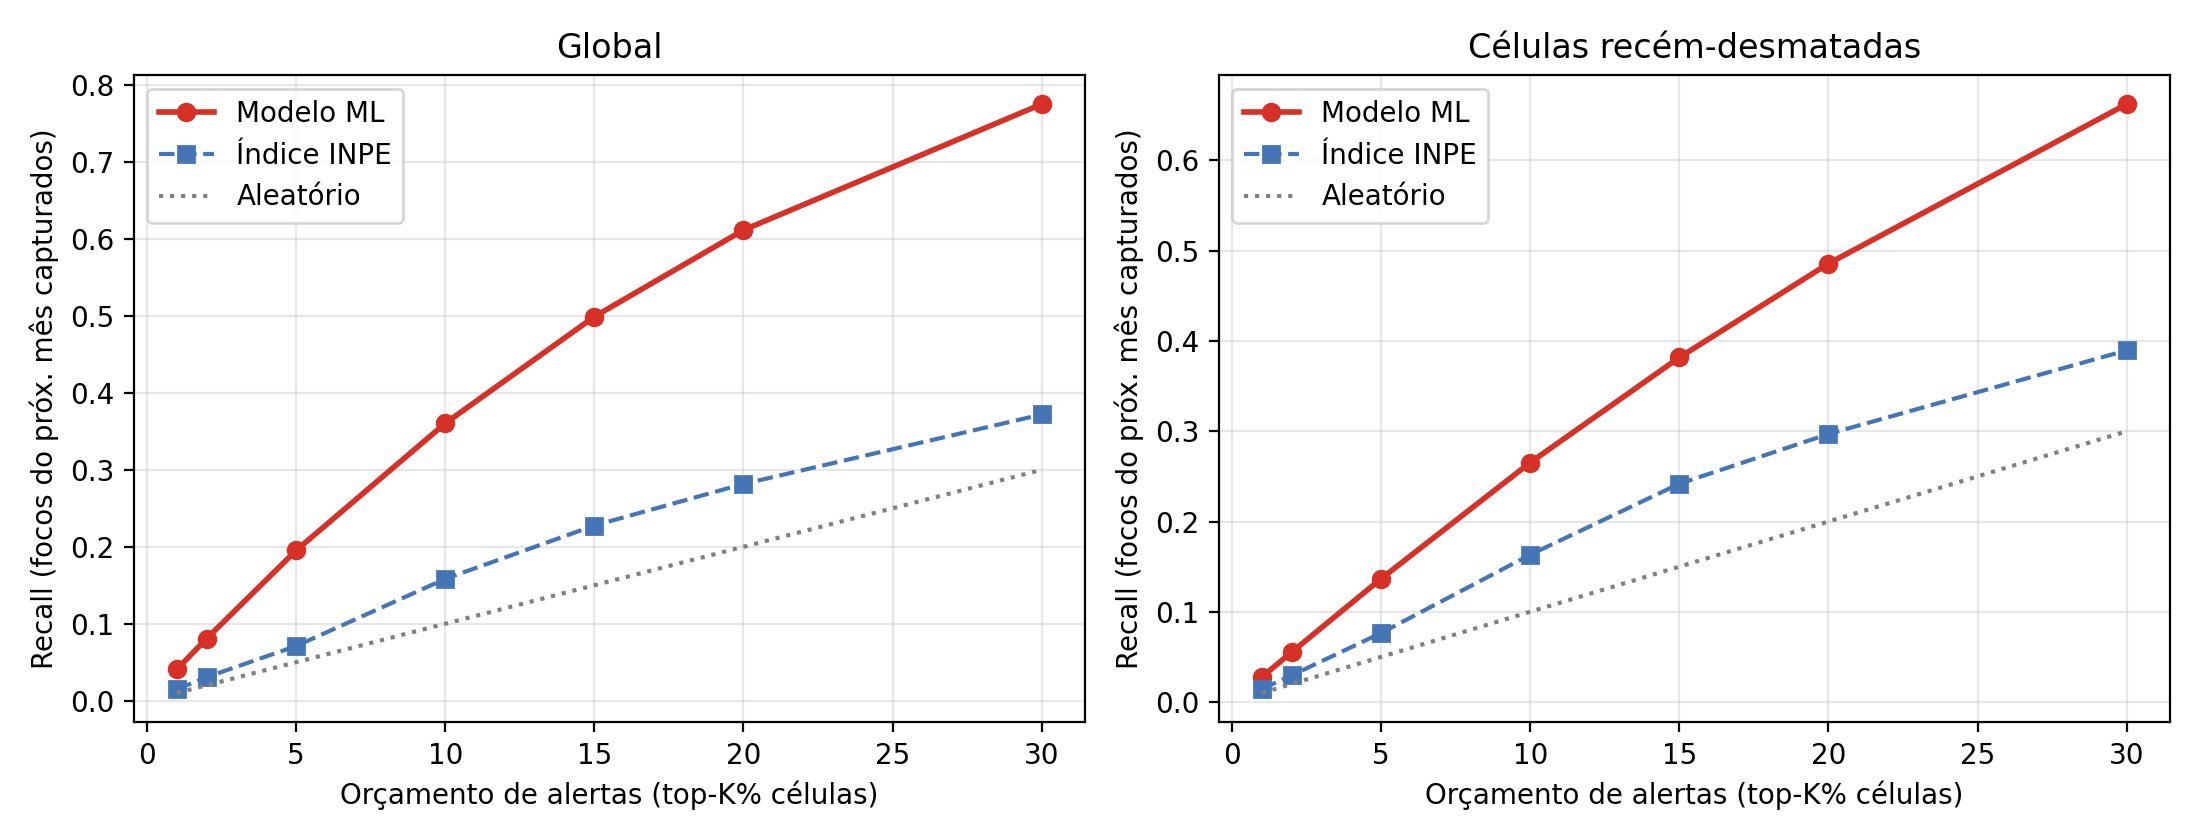
\includegraphics[width=\textwidth]{modelos/relatorios/avaliacao_operacional_recall_k.png}
\caption{\emph{Recall@K} em função do orçamento de alertas (modelo ML vs.\ índice INPE vs.\ aleatório), global (esq.) e em células recém-desmatadas (dir.).}
\label{fig:oco_recallk}
\end{figure}

\paragraph{Horizonte de previsão.} Estendendo o alvo para \(t+2\) e \(t+3\) meses, o
\emph{skill} permanece \textbf{estável} (PR-AUC \numlist{0,779;0,779;0,781} para \(t+1\),
\(t+2\), \(t+3\); Figura~\ref{fig:oco_horizonte}), sem o decaimento típico. Isso confirma
que a ocorrência mensal de fogo é governada por componentes \emph{lentos} (sazonalidade,
histórico de fogo, desmatamento), e não por dinâmica meteorológica de curto prazo ---
um resultado operacionalmente favorável, pois fornece \textbf{até um trimestre de
antecedência} sem perda de desempenho. A contrapartida honesta é que o modelo captura o
regime sazonal/persistente, não a dinâmica sub-mensal; previsões em escala mais fina
exigiriam outra formulação.

\begin{figure}[h]
\centering
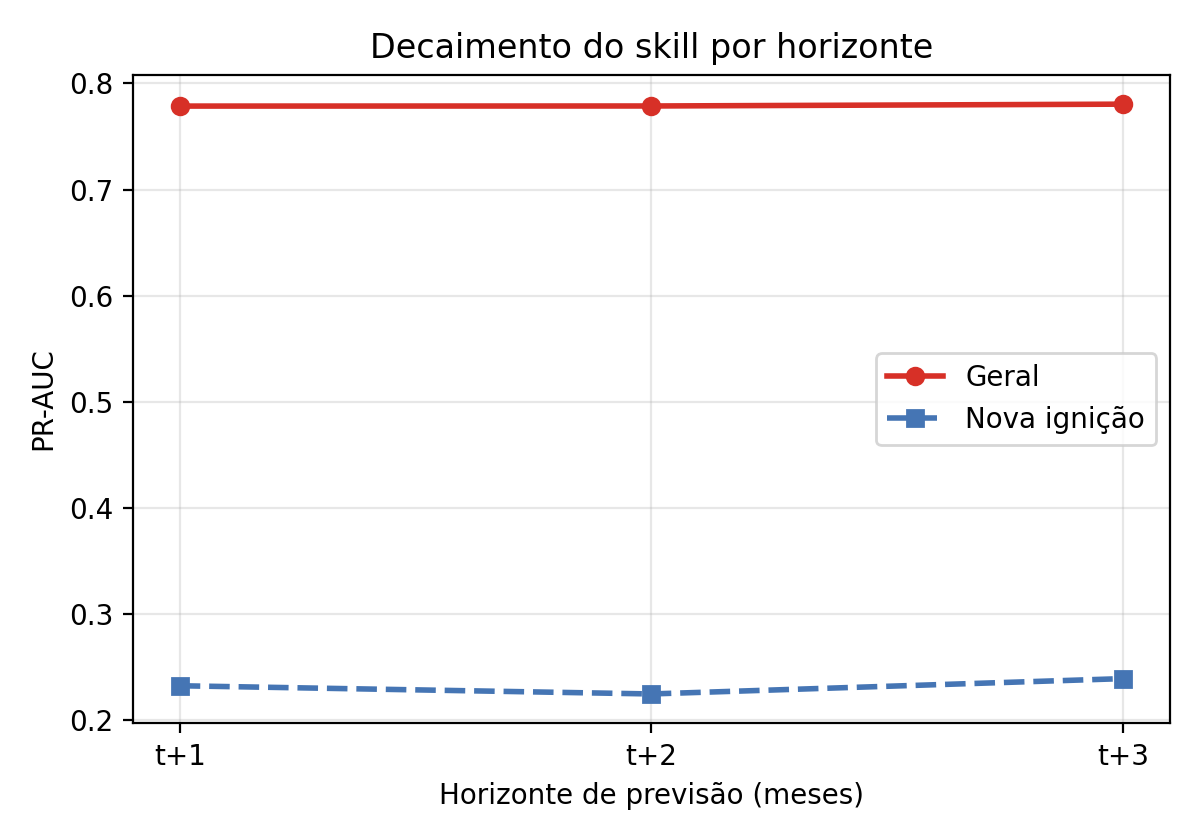
\includegraphics[width=0.6\textwidth]{modelos/relatorios/avaliacao_horizonte.png}
\caption{Decaimento do \emph{skill} (PR-AUC) por horizonte de previsão (\(t+1\) a \(t+3\) meses): estável, geral e na nova ignição.}
\label{fig:oco_horizonte}
\end{figure}

\section{Integração ao produto}
\label{sec:oco_produto}

O modelo final (base + desmatamento) foi serializado, calibrado por \emph{conformal}
(cobertura \num{0,900}) e exposto como produto: uma previsão por célula de \(P(\text{fogo no
próximo mês})\) com rótulo conformal e \emph{drivers}, servida por aplicação \emph{Flask} com
mapa interativo, independente do aplicativo de \emph{nowcast}. Verificações de sanidade
conferem com a fenologia do fogo (p.ex.\ Roraima com alto risco em dezembro; sul do Pará
baixo em dezembro, cuja estação de fogo é julho--outubro).

\section{Síntese}
\label{sec:oco_sintese}

Os experimentos, sob validação honesta, sustentam uma tese coesa: (i) na escala
mensal/\SI{0,25}{\degree}, a ocorrência de fogo é dominada por persistência espaço-temporal e
sazonalidade, o que torna redundantes a reanálise meteorológica (e o FWI) e a acessibilidade
estática; (ii) o modelo de ML \emph{supera} os índices físicos operacionais na previsão de
fogo observado; (iii) o gargalo é a \textbf{nova ignição}, e o único sinal útil ali é o
\textbf{desmatamento recente}, reposicionando o alerta precoce como, em primeira ordem, um
problema de detecção de fronteira de desmatamento; (iv) a incerteza é quantificável com
garantia estatística. A reformulação eleva o trabalho de ``reprodução de um índice'' para
``previsão de fogo observado validada contra a realidade e contra o índice físico'', com um
teto de desempenho honestamente caracterizado.
